\vfill\documentclass[12pt]{extarticle}

%PA
\usepackage{csvsimple}
\usepackage{float}
\usepackage{dirtree}
\usepackage{paralist}
\usepackage{extarrows}
\usepackage{svg}
\usepackage{caption}
\usepackage{subcaption}


%Code
%\usepackage[disable]{todonotes}
\usepackage{todonotes}
\usepackage{listings}
\usepackage{xcolor}
\usepackage[utf8]{inputenc}
\usepackage{amsmath}
\usepackage{titlesec}
\usepackage{pdfpages}
\usepackage{pdflscape}
\usepackage{amssymb}
\usepackage{rotating}
\usepackage{verbatim}
\usepackage[justification=centering]{caption}
\usepackage{csquotes}
\usepackage{wasysym}
\usepackage[ngerman]{babel}
%\usepackage[backend=biber,style=numeric,sorting=nyt]{biblatex}
\usepackage{hyperref}
\usepackage{lastpage}
\usepackage{hyperref}
\usepackage[a4paper, left = 2.8cm, right = 2.8cm, top=1.5cm , bottom = 1.5cm, includeheadfoot]{geometry}
\usepackage[style=numeric]{biblatex}
\addbibresource{literatur.bib}
\usepackage{enumitem}

\usepackage{parskip}
\setlength{\parindent}{0pt} 
\setlength{\parskip}{0.8em}


\setlength{\parindent}{0em} %Absätze nicht einrücken

\usepackage{fancyhdr}
\pagestyle{fancy} %eigener Seitenstil
\fancyhf{} %alle Kopf- und Fußzeilenfelder bereinigen
\fancyhead[L]{\nouppercase{\leftmark}} %Kopfzeile links
\fancyhead[C]{} %zentrierte Kopfzeile
\fancyhead[R]{} %Kopfzeile rechts
\renewcommand{\headrulewidth}{0.4pt} %obere Trennlinie
\fancyfoot[C]{\thepage} %Seitennummer
\renewcommand{\footrulewidth}{0.4pt} %untere Trennlinie


% Links
% https://www.nm.ifi.lmu.de/pub/Fopras/schw14/PDF-Version/schw14.pdf



\title{Bachelorthesis}

\author{Philipp Altnickel}
\begin{document}
\begin{titlepage}
	\centering
	
\includegraphics[width=0.49\textwidth]{Logo_HSB_Hochschule_Bremen.png}
	
\includegraphics[width=0.49\textwidth]{Logo_HEC.png}
	\par
	\vspace{2cm}
	{\large \textbf{Masterthesis}\\Fakultät 4 Elektrotechnik und Informatik\\Informatik M. Sc. (Komplexe Softwaresysteme)\par}
	\vspace{2cm}
	{\LARGE\bfseries Prozessoptimierung der Stückgutverladung auf LKW im Hafenterminal innerhalb von gebuchten Zeitfenstern\par}
	\vspace{3cm}
	{\large \textbf{Eingereicht von:} Philipp Altnickel (5049547)\par}
	{\large \textbf{Abgabetermin:} 29.11.2024\par}
	\vspace{1cm}
	{\large \bfseries zum Erlangen des akademischen Grades\par\LARGE Master of Science (M.Sc.)\par}
	
	\vfill
	
	{\large \textbf{Erstprüfer:} Prof. Dr. Lars Braubach (Hochschule Bremen)\\\textbf{Zweitprüfer:} André Stadtelmeyer (HEC GmbH)\par}
\end{titlepage}
\newpage

\setcounter{page}{2}

\phantomsection
\subsection*{Erklärung über das eigenständige Erstellen der Arbeit}

Hiermit versichere ich, dass ich die vorliegende Arbeit selbstständig verfasst und keine anderen als die angegebenen Quellen und Hilfsmittel benutzt habe. Die Stellen der Arbeit, die anderen Werken dem Wortlaut oder dem Sinn nach entnommen wurden, sind durch Angaben der Herkunft kenntlich gemacht.

Diese Erklärung erstreckt sich auch auf in der Arbeit enthaltene Grafiken, Skizzen, bildliche Darstellungen sowie auf Quellen aus dem Internet.
Die Arbeit habe ich in gleicher oder ähnlicher Form auch auszugsweise noch nicht als Bestandteil einer Prüfungs- oder Studienleistung vorgelegt. 

Ich versichere, dass die eingereichte elektronische Version der Arbeit vollständig mit der Druckversion übereinstimmt.
\\ \\ \\

\makebox[6cm]{\hrulefill}\hfill\makebox[6cm]{\hrulefill}\\
Ort, Datum \hfill Philipp Altnickel\\
\mbox{}\hfill(Matr.-Nr. 5049547)



\newpage
\phantomsection
\section*{Abstract}
\addcontentsline{toc}{section}{Abstract}
\todo[inline]{Schreiben}



\newpage
\tableofcontents

\newpage
\pagestyle{fancy}

\section{Einleitung}

\todo[inline]{TODOs: -Prüfen, ob alle Figures auf im Text referenziert und besprochen werden; - Stapler/Gabelstapler einheitlich; - Organisation bei der Arbeit Kanban o.ä. beschreiben?, Allgemein Methodik u.a. Interviews geführt; -Einfache Links, u.a. Baeldung, GeeksForGeeks als Fußnote?!}

%Das folgende Kapitel soll zunächst eine Einführung in die in dieser Arbeit betrachtete Problemstellung, sowie in Ziele und Ansätze zur Umsetzung geben.

In Zeiten von globaler Wirtschaft mit weltweitem Handel ist die Schifffahrt ein zentraler Pfeiler und wichtiger Bestandteil der Lieferketten zwischen entfernten Ländern und Kontinenten. Mit stetig steigender Menge von ausgetauschten Gütern und gleichzeitig wachsendem Preisdruck wird es immer wichtiger, die gesamte Prozesskette so schnell und günstig wie möglich zu gestalten. Dies gilt insbesondere auch für die Infrastruktur in den Häfen. 

\subsection{Problemstellung}

Die vorliegende Arbeit beschäftigt sich mit einem ganz konkreten und aus der Praxis stammenden Thema im dem Bereich der Hafenlogistik. Zum An- und Abtransport von Waren, die noch verschifft werden sollen oder bereits auf diesem Wege geliefert wurden, wird neben dem Güterverkehr auf der Schiene vor allem der LKW als bedeutendes Transportmittel genutzt \todo{Quellen? Evtl. Graphen zur Verteilung bei Analyse des Problemfelds, um die Bedeutung des LKW deutlich zu machen}. Im Gegensatz zur Containerverladung, welche aufgrund der einheitlichen Größen schon sehr standardisiert und optimiert ist, soll es in dieser Arbeit um die Verladung von Stückgütern von und auf LKW gehen. Diese Arbeit ist in Zusammenarbeit mit der HEC GmbH entstanden und beschäftigt sich deshalb auch mit einem Problem, welches in aktuellen Projekten für die Häfen in Hamburg und Bremerhaven\todo{Häfen benennen} aufgetreten ist. Momentan gibt es dort eher einfach gehaltene Softwaresysteme, über die LKW Fahrer ihre geplante Lieferung bzw. Abholung in festgelegten Zeitslots avisieren können. In jeden Zeitrahmen können allerdings mehrere LKW gebucht werden. Die Verteilung und Reihenfolge der Abfertigung läuft dabei nach keinem organisierten System, sondern eher zufällig bzw. nach Reihenfolge der Buchung. Dies führt allerdings dazu, dass die Abfertigung von Zeit und Aufwand nicht besonders optimal abläuft. Eine Berücksichtigung bspw. von benötigter Lademaschine, Verfügbarkeit von Personal oder Lagerplatz könnte hier zu Zeit- und somit Geldersparnissen bei Terminal und LKW Fahrer führen. 

\subsection{Ziele der Arbeit}

Ziel dieser Arbeit soll es sein, eine softwarebasierte Lösung bzw. Optimierung für das zuvor beschriebene und relativ spezifische Problem zu finden. Ganz konkret heißt dies, einen Algorithmus zu entwickeln, welcher die benötigte Abfertigungszeit pro LKW durch geschickte Planung reduzieren kann bzw. so dafür sorgt, dass mehr LKW in gleicher Zeit bearbeitet werden können. Da es sich um einen durchaus komplexen Kontext handelt, der auch in vielen Details nicht direkt mit anderen Terminals zu vergleichen ist, wird ein erster wichtiger Teil dieser Arbeit die Analyse der Dimensionen des Problems mit anschließender Anforderungsanalyse sein. Dabei geht es darum, alle Regeln, Abhängigkeiten und Parameter zu verstehen, die in einer Optimierung bedacht werden sollten. Dies wird allerdings sehr komplex sein und auch einige schlecht oder gar nicht planbare Unsicherheiten beinhalten. Ziel dieser Arbeit wird deshalb keine hoch genaue und technische Optimierung des Problems sein. Viel mehr soll hier der Gesamtkontext bearbeitet werden, verschiedene technische Möglichkeiten zur Umsetzung abgewogen werden und anschließend anhand einer prototypischen Planung und Umsetzung die Machbarkeit der theoretischen Betrachtung gezeigt werden. Auch wenn nicht alle Aspekte praktisch berücksichtigt werden können, wird der gesamten Entwicklungsprozess viele Erkenntnisse zu Problemen, Herausforderungen und Möglichkeiten liefern. Auch dies ist ein wichtiges Ergebnis für eine mögliche anschließende reale Umsetzung.

\subsection{Lösungsansatz}

Momentan wird hier in der Regel ein sehr statisches System zur Buchung von Zeitslots durch die LKW Fahrer bzw. deren Speditionen verwendet. Unter Angabe einiger Details zur gelieferten, bzw. zu holenden Ware, können feste Zeiträume gebucht werden, in denen die LKW in den Hafen einfahren und ihre Lieferung durchführen dürfen. Die Idee ist vor allem, eine Optimierung der Abfertigung innerhalb eines Zeitslots zu finden. Die Vergabe der Slots selbst ist dabei wenig variabel. Im Gegensatz zu vielen anderen Anwendungsbereichen steht hier hinter den gelieferten Waren kein sich wiederholender und somit gut planbarer Produktionsprozess und auch die Art der Waren variiert stark. Der Ladeprozess selbst hängt von sehr vielen Faktoren ab, z.B. Verfügbarkeit von Ladehilfsmitteln, Personal oder Stellplätzen. 

Nach einer ausführlichen Erfassung der Rahmenbedingungen, wird es darum gehen, konkrete Anforderungen an eine Optimierung zu formulieren. Ein festgelegter Satz von wirklich wichtigen Eingabedaten ist der erste Schritt für eine sinnvolle Optimierung. Das Hauptziel dieser Arbeit ist es dann, technische Möglichkeiten zur Lösung zu planen und umzusetzen. Die Herausforderung ist es sein, alle Anforderungen zu berücksichtigen und gleichzeitig den Zeitbedarf pro abgefertigtem LKW möglichst weit zu verringern bzw. möglichst viele zusätzliche LKW bearbeiten zu können. Dies ist kein geradliniger Prozess mit einer einzigen, korrekten Lösung, sodass diese Arbeit auch dazu dienen soll, verschiedene Ansätze praktisch auszuprobieren und zu vergleichen. Neben der Recherche und Ausarbeitung von vielversprechenden Methoden, wird auch die Evaluation und Bewertung dieser Ansätze ein wesentlicher Aspekt dieser Arbeit sein. Ein quantitativer Vergleich der Ergebnisse zueinander und auch zur Ausgangssituation kann belegen, ob die entwickelten Algorithmen grundsätzlich funktionieren. Sie erlauben aber auch eine Einschätzung zu möglichen Potenzialen und Höhen der Verbesserung.



\newpage
\section{Grundlagen}
Den Beginn dieser Arbeit bildet die Erläuterung einiger Grundbegriffe und Technologien, die im weiteren Verlauf genutzt werden.

\subsection{Künstliche Intelligenz (KI)}
\label{section:ki}


\subsection{Job Shop Scheduling?}
% ??? oder Scheduling allgemein?

\subsection{Traveling Salesman Problem (TSP)}
\label{sec:grundlagen_tsp}
\todo{NP-schwer erwähnen?!}

Das Traveling Salesman Problem, im deutschen auch bekannt als das Problem des Handlungsreisenden, ist ein schon sehr altes Problem der theoretischen Informatik. Es handelt sich dabei um ein kombinatorisches Optimierungsproblem. Die Problemstellung selbst ist dabei sehr einfach erklärt: Ein Handlungsreisender möchte eine Menge von Stationen mit einer möglichst kurzen Reisestrecke besuchen. Jede Station soll dabei genau einmal besucht werden und die erste Station ist gleich der letzten, sodass ein Kreis entsteht. Ziel der Optimierung ist es also, die best mögliche Reihenfolge der zu besuchenden Orte zu finden (ein beispielhaftes Problem ist in Abb. \ref{fig:tsp_deutschland} dargestellt). \cite{travelingSalesman}

\begin{figure}[H]
    \centering
    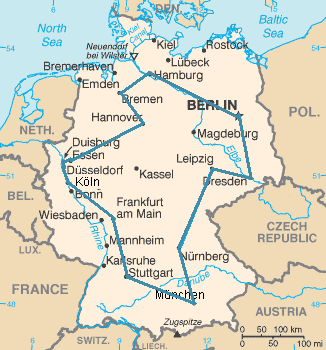
\includegraphics[width=0.5\textwidth]{images/TSP_Deutschland_3.png}
    \caption{TSP Beispiel - Beste Reiseroute durch die 15 größten Städte in Deutschland \cite{tspDeutschland}}
    \label{fig:tsp_deutschland}
\end{figure}

Modellieren lässt sich das Problem als Graph, bei dem die Knoten den Städten entsprechen und Kanten mit Gewichtungen den Aufwand der Reise zwischen diesen Städten darstellen. Das Problem der optimalen Wegfindung innerhalb eines Graphen lässt sich aber auch eine Vielzahl von anderen Problemen übertragen. Es hat somit eine große Bedeutung innerhalb der Informatik. Das möglichst schnelle Finden einer möglichst guten Lösung kann viele Probleme lösen, weshalb es bis heute Bestrebungen zur Suche nach guten Lösungsverfahren gibt. \cite{travelingSalesman} Das TSP ist allerdings ein sehr komplexes Problem, es gibt keine bekannte, effiziente Lösung dafür. Die Schwierigkeit ist, dass die Zahl der Kanten exponentiell der Zahl der Knoten n steigt. Sie folgt der Formel $n(n-1)/2$ \cite{graphenEckenKanten}. Ein vollständiger Graph aus vier Knoten hat so beispielsweise sechs Kanten, während es für fünf Knoten schon zehn Kanten und für zehn Knoten braucht es bereits 45 Kanten.

Lösungsverfahren teilen sich in exakte und heuristische Verfahren auf. Exakte Verfahren gehen meist alle Wege oder zumindest einen Großteil der möglichen Wege durch. Sie liefern dabei immer das best mögliche Ergebnis, können aber durchaus hohe Berechnungszeiten haben. Heuristische Verfahren versuchen dagegen basierend auf Erfahrungswerten, möglichst schnell eine gute Lösung zu finden. Diese kommen dem oft sehr nah aber selten an diesen heran. \cite{travelingSalesman}

Eine Erweiterung des TSP ist das multiple Traveling Salesmen Problem (mTSP). Statt einem einzelnen Handlungsreisenden sollen hier Wege für mehrere Reisende gefunden werden, sodass jede Station von genau einem der Handlungsreisenden besucht wird. \cite{mtsp}

\subsection{Versuchsauswertung}
\todo{Quellen}
% Median, Mittelwert, Standardabweichung, ...

Ein sehr wesentlicher Teil dieser Arbeit wird sich mit der Auswertung der Arbeitsergebnisse beschäftigen. Dabei werden Messergebnisse erhoben und mit grundlegenden statistischen und mathematischen Verfahren ausgewertet, welche hier noch einmal kurz erläutert werden.

\subsubsection{Arithmetisches Mittel} \todo{von wikipedia, bessere Quelle?}

Das arithmetische Mittel, oft auch Durchschnitt oder Mittelwert genannt, beschreibt des typischen Wert einer Verteilung. Es beschreibt die Tendenz bzw. das Zentrum, um die sich alle anderen Werte verteilen. Berechnen lässt es nicht nach Formel \ref{eq:arithmMittel}, also der Summe aller Werte dividiert durch die Anzahl an Werten. Dieser Wert gibt schin einmal einen guten Eindruck, in welchem Bereich die verteilten Werte etwa liegen.

\begin{equation} \label{eq:arithmMittel}
\mu=\frac{1}{n} \sum_{i=1}^n x_i
\end{equation}

\subsubsection{Standardabweichung} \todo{https://de.statista.com/statistik/lexikon/definition/126/standardabweichung/, bessere Quelle?}

Die Standardabweichung ist ein Maß für die Streuung der Werte um das arithmetische Mittel. Sie lässt sich nach Formel \ref{eq:standardAbw} berechnen. Sie summiert alle Quadrate der Abweichung vom Mittelwert und zieht aus allem die Quadratwurzel. 

\begin{equation} \label{eq:standardAbw}
    \sigma=\sqrt{\sum_{i=1}^{n}\left(x_{i}-\mu\right)^{2}}
\end{equation}

Nimmt man an, dass die Werte normalverteilt sind, so lässt sich ableiten, dass im Bereich des Mittelwertes $\pm$ der Standardabweichung ca. 68\% aller Werte liegen und im Umkreis der doppelten Standardabweichung sogar ca. 95\% der Werte. Aus einer hohen Standardabweichung lässt sich also folgern, dass viele Werte sehr weit um den Mittelwert gestreut sind, es kann also durchaus oft vorkommen, dass viele Werte sehr weit vom Durchschnitt entfernt liegen. Dagegen bedeutet eine geringe Standardabweichung, dass sehr viele Werte nah am arithmetischen Mittel liegen und dieser so ein sehr gutes Bild über die Werte geben, welche in der Regel vorkommen.

\begin{figure}[H]
    \centering
    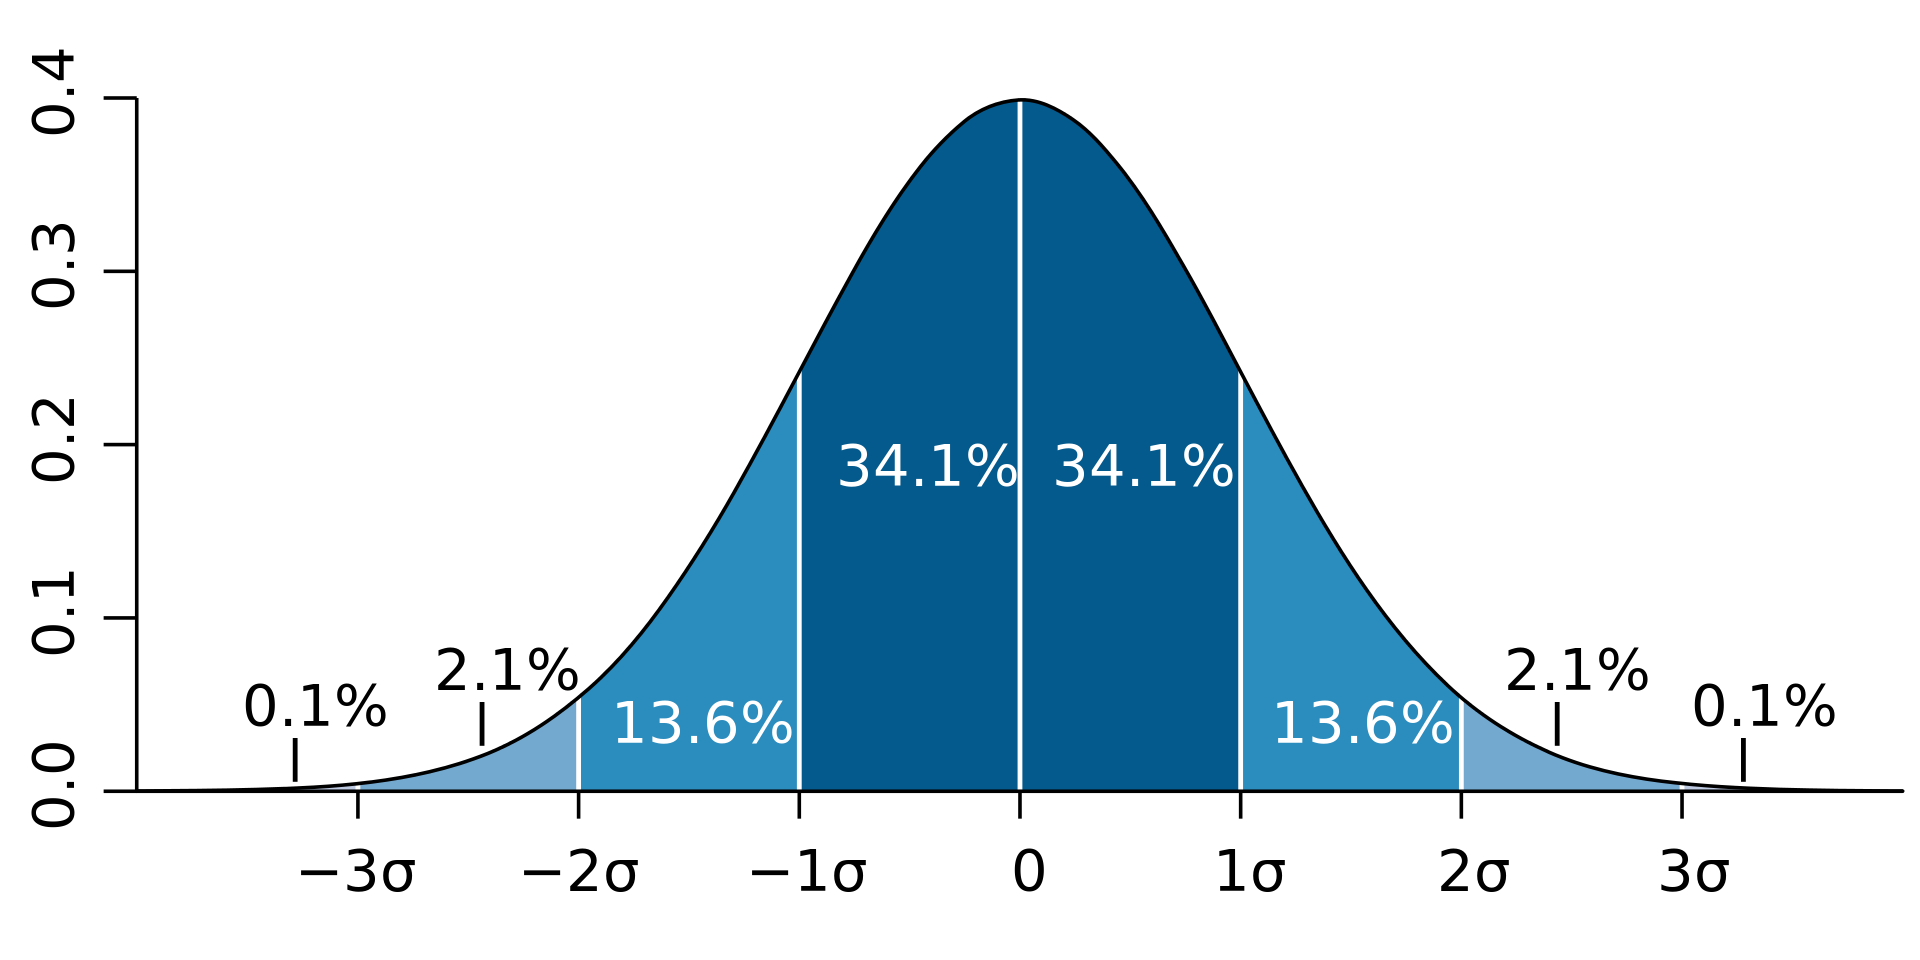
\includegraphics[width=0.5\textwidth]{images/Normalverteilung.png}
    \caption{Intervalle um den Mittelwert einer Normalverteilung \cite{normalverteilung}}
    \label{fig:normalverteilung}
\end{figure}


\subsection{R und RStudio}

R ist eine im Jahr 1992 entwickelte Programmiersprche bzw.- umgebung, um statistische Auswertungen und Grafiken zu erzeugen. Sie enthält bereits viele Funktionen zu diesem Zweck, kann aber auch sehr leicht durch Bibliotheken erweitert werden. Auswertungen und Grafiken haben eine entsprechende Qualität, um direkt in Veröffentlichungen genutzt zu werden. Insbesondere für sich wiederholende Auswertungen kann es sehr sinnvoll sein, eigene Skripte mit R zu schreiben und diese wiederholt auszuführen. Daten können beispielsweise sehr leicht aus gängigen Datenformaten wie CSV importiert und verarbeitet werden. Die Sprache hat eine relativ große Bekanntheit und Community, was eine Entwicklung und das finden von speziellen Lösungen sehr einfach macht. \cite{r}

RStudio ist eine für R entwickelte Entwicklungsumgebung, die eine einfachere Handhabung möglich macht. Eine grafische Benutzeroberfläche, Syntaxhighlighting, automatische Codeeinrückung o.ä., wie es aus Entwicklungsumgebungen vieler anderer Sprachen bekannt ist, machen die Bedienung sehr viel einfacher, als es noch zum Beginn der Entwicklung von R der Fall war. \cite{rstudio}


 % aktuell 2 Seiten


\newpage
\section{Analyse des Problemfelds}
\label{sec:analyse}
Den eigentlichen Beginn dieser Arbeit soll nun eine Ausarbeitung des Problemfelds machen. Es handelt sich um ein sehr umfangreichen Themenkomplex, welcher durch die kurze einleitende Beschreibung nicht komplett zu erfassen ist. Teil dieser Arbeit ist es deshalb an dieser Stelle zunächst zu analysieren, in welchen Kontext die Problemstellung einzuordnen ist und auch genauer zu erarbeiten, welche Dimensionen dort hineinspielen. Es sollen also Details des Problems herausgearbeitet werden und daraus mögliche Potenziale und Ansätze für die nachfolgende Optimierung erkannt werden.

\subsection{Verwandte Arbeiten} 
\todo{Aus Expose kopiert, nochmal überarbeiten?}

Die Problemstellung stellte sich schon bei erster genauerer Betrachtung als durchaus komplex heraus. Das Thema Zeitslotplanung ist im gesamten Bereich Logistik und sogar darüber hinaus von Bedeutung, es gibt somit schon viel Vorarbeit und Literatur in diesem Bereich. Allerdings sind die Anforderungen und Rahmenbedingungen überall sehr unterschiedlich und es lassen sich kaum allgemeine Lösungen finden. Selbst im Bereich der Hafenlogistik gibt es zwischen verschiedenen Häfen, Terminals und Gütern verschiedenste Verfahren und Regelungen.

Es gibt durchaus einige Arbeiten, die sich in einem ähnlichen Rahmen bewegen, also ebenfalls das Thema Zeitslotmanagement in Zusammenhang mit LKW Abfertigung betrachten. In der Regel geht es dabei eher um die effiziente Vergabe der Slots selbst. Beispielsweise darum, wie ankommende LKW möglichst effizient und ohne Zeitverlust auf spezifische und zweckgebundene Laderampen verteilt werden können (siehe \cite{truckDockAllocation}). Weitere Arbeiten beschäftigen sich sogar noch konkreter mit Zeitslotmanagement im Kontext von Hafenterminals, allerdings für Container (siehe \cite{vergleichbareArbeiten2}, \cite{vergleichbareArbeiten1}). Es gibt auch ein Beispiel zur adaptiven Planung von Zeitfenstern, basierend auf Echtzeitdaten der LKW (siehe \cite{vergleichbareArbeiten3}). 

Die meisten dieser Arbeiten beschäftigen sich direkt mit der Planung und Vergabe der Slots selbst. Die Optimierung dieser Arbeit soll hauptsächlich innerhalb dieser Slots stattfinden. Bei der Zeitplanung wird sehr auf die Wünsche der Speditionen eingegangen und es gibt im hier betrachteten Beispiel auch keinen so klar strukturierten Produktionsprozess gibt, wie es möglicherweise in anderer, zuvor genannter Literatur der Fall ist. Der Fokus soll eher darauf liegen, den Lade- und Abladeprozess selbst zu verbessern. Durch verbesserte Verteilung und Sortierung innerhalb des Slots können die in dem Prozess benötigten Ressourcen womöglich besser ausgenutzt werden und so mehr LKW in der gleichen Zeit abgefertigt werden.


\subsection{Ausgangszustand vor dieser Arbeit}

Bei dem hier bearbeiteten Thema handelt es sich um eine sehr spezifische Problematik. In dieser Form gibt es also keine direkten Quellen, auf die aufgebaut werden könnte und aus denen eine Grundlage für die weitere Arbeit gezogen werden kann. Da hier eine Lösung für die spezifischen Softwareprojekte der HEC für die Terminals von Unikai und BLG in Hamburg und Bremerhaven geschaffen werden soll, wurde die folgende Ausarbeitung stattdessen auf Basis von Experteninterviews durchgeführt (siehe Anhang \ref{sec:appendixInterviews}\todo{richtiger Verweis}). Außerdem wurde die bisher eingesetzte Software über einen für diese Arbeit zur Verfügung gestellten Testzugang genauer begutachtet. 

\subsubsection{Aktueller Bearbeitungsprozess}

Prinzipiell teilt sich der ganze Bearbeitungsprozess eines LKW in zwei wesentliche Abschnitte. Zunächst einmal gibt es eine Reihe von Schritten, die ablaufen müssen, bevor ein LKW physisch im Hafen ankommt. Im allerersten Schritt gibt es eine Vorankündigung der Liefergüter. Die sogenannte Avise wird durch die Reeder, also die Eigentümer bzw. Betreiber der Schiffe angemeldet. Durch diese Avise erhält das Terminal schon einmal grundlegende Informationen zu den Gütern, welche zukünftig den Hafen durchlaufen werden. Zu den hier übermittelten Informationen zählt neben einer eindeutigen Buchungsnummer zunächst die Angabe um welchen der drei möglichen Warentypen Container, Stückgut oder Fahrzeug es sich handelt. Für Fahrzeuge und Container werden hier auch Informationen zu den genauen Warenpositionen, also Fahrzeugidentifikationsnummer (FIN) oder Containernummer und ISO-Nummer las Angabe der Containergröße übergeben. Für Stückgüter, welche den Hauptfokus dieser Arbeit darstellen, gibt es keine genauen Angaben zu den Packstücken. Hier kann es mehrere Packstücke unterschiedlicher Art geben, z.B. einen zerlegten Raupenkran. Außerdem werden durch den Reeder noch Ankunfts- (Expected Time of Arrival, ETA) bzw.Abfahrtszeit (Expected Time of Departure, ETD) des Schiffes gelierfert.

Wollen Speditionen oder Fahrer nun einzelne dieser Güter liefern oder abholen, so können diese dann für zuvor avisierte Güter einen Slot buchen. Dazu geben diese zunächst eindeutige Nummern zur Identifikation der Ware ein, wie FIN oder Buchungsnummer. Anhand dessen kann zunächst geprüft werden, ob bereits eine Avise durch den Reeder erfolgt ist. Im positiven Fall können nun noch einmal spezielle Informationen zu den auf dem LKW befindlichen Gütern angegeben werden. Dies können Anzahl, Gewicht oder Maße sein, aber auch Zusatzinformationen, u.a. ob es sich beispielsweise um Gefahrgut oder Zollware handelt. Im Anschluss daran kann ein verfügbarer Zeitslot gewählt werden. Die Verfügbarkeit richtet sich dabei nach mehreren Faktoren. Einmal muss die Ware bis zu einen Tag vor Abfahrt bzw. ab einen Tag nach Ankunft des Schiffes geliefert bzw. abgeholt werden. Außerdem werden bereits hier Abfertiungsbereiche für die spätere Be- und Entladung ermittelt. Jeder Bereich hat hier einen maximalen Vorlauf, wie weit im Voraus gebucht werden kann. In Kombination mit der Anzahl der bereits gebuchten LKW werden aus all diesen Faktoren die verfügbaren Slots angezeigt. Die Anzahl von möglichen LKW pro Slot wird dabei aus Erfahrungswerten bestimmt. Eine Variation über den Tag wird hier auch nur über Erfahrungswerte zu z.B. Pausenzeiten vorgenommen, in denen weniger LKW schaffbar sind. Grundsätzlich wird in den hier betrachteten Terminals mit einstündigen Slots gearbeitet, wobei die Anzahl der LKW die in den Abfertigungsbereichen in dieser Zeit geschafft werden sehr stark schwankt. Die Verfügbarkeit von Laderessourcen unterscheidet sich je nach Bereich sehr und auch die Zeiten für jeden Gütertyp. So lassen sich Container oft sehr schnell abarbeiten, während Stückgüter schon einmal sehr viel Zeit in Anspruch nehmen können und Fahrzeuge liegen zeitlich dazwischen.

Nach erfolgter Anmeldung kann der LKW Fahrer dann zu einem beliebigen Zeitpunkt innerhalb des ausgewählten Slots im Terminal erscheinen und die angekündigte Ware anliefern oder abholen.
\todo{Nach Interview Claas}

\subsubsection{Aktuell genutzte Software}

% - Slotsystem mit festen 1h Slots
% - Eingabemaske für grobe Daten zur Lieferung: Sendungsnr, Größe, Gewicht, Freitextbeschreibung, ...?
% - Wie werden die Daten gespeichert und weiterverarbeitet?
% - Wie wird die Reihenfolge aktuell festgelegt?

Momentan wird eine durch die Firma HEC entwickelte Software eingesetzt und ermöglicht eine Slotbuchung und -steuerung. Sie ist einmal als Desktop Variante verfügbar, was hauptsächlich von Spediteuren genutzt wird. Eine Mobile App kann von LKW Fahrern genutzt werden, um auch unterwegs entsprechende Daten mit einem Smartphone übermitteln zu können. Erfasst werden dabei grobe Daten zu der Sendung und den entsprechenden Gütern. Danach können die Nutzer einen verfügbaren Zeitslot auswählen, in dem sie die benannte Ware anliefern, bzw. abholen möchten. 

Über eine Eingabemaske (siehe Abb. \ref{fig:eingabemaske_aktuelles_system}) können Daten zur Buchung bzw. zu den Gütern, welche er laden oder abholen will eingeben. Dazu gehören u.a. die Buchungsnummer, eine Warenbezeichnung, sowie Anzahl, Größe in Länge/Breite/Höhe und Gewicht. Anschließend gibt es die Möglichkeit, einen Slot auszuwählen, in dem der angemeldete LKW kommen möchte und abgefertigt wird.

\begin{figure}[H]
    \centering
    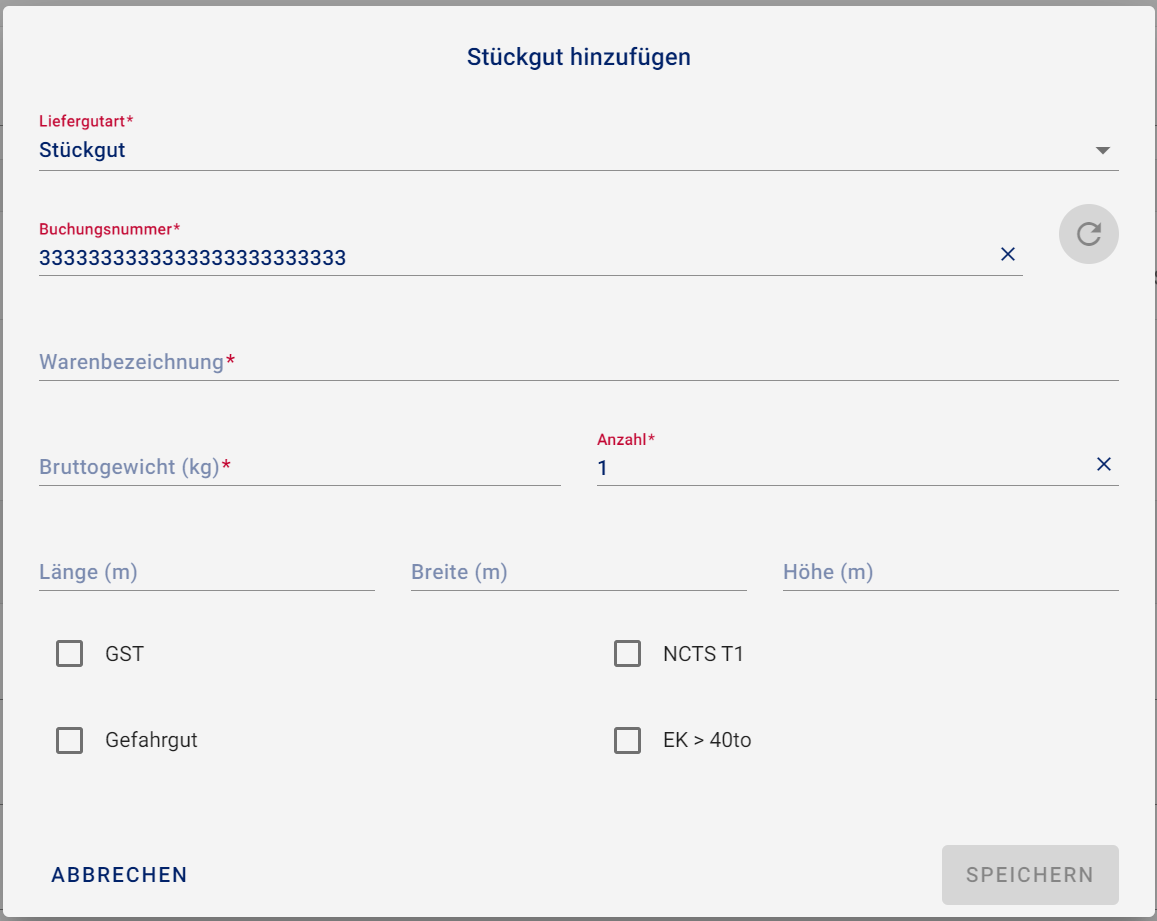
\includegraphics[width=\textwidth]{images/Eingabemaske_aktuelles_System.png}
    \caption[Eingabemaske für LKW Fahrer im aktuell genutzten System]{Eingabemaske für LKW Fahrer im aktuell genutzten System \\ (GST = Großraum- und Schwertransport, NCTS T1 = Zollfreigabe, EK = Einzelkolli/Einzelelement)}
    \label{fig:eingabemaske_aktuelles_system}
\end{figure} 

Alternativ, bzw. ergänzend zur Eingabe über die zuvor beschriebene Anwendung, kann eine Anmeldung automatisiert im EDI-Format erfolgen. Das \glqq{}electronic data interchange\grqq{} Format ist ein standardisiertes Format zum Datenaustausch, welches vor allem in der Schifffahrt noch weit verbreitet ist. Auch hier können erste Daten zum jeweiligen Gut übermittelt werden, ohne eine manuelle Eingabe. Dass das Format standardisiert ist, heißt allerdings auch hier nicht, dass alle übermittelten Daten vollständig und gut sind. Viele Daten, insbesondere die Qualität Beschreibungen hängen auch hier von stark von den bearbeitenden Mitarbeitern ab. \todo{Erklärung/Darstellung EDI und einer Beispiel Message, Quelle?}

Das Terminal hat für das ganze System die Möglichkeit eine Anzahl von LKW einzustellen, welche die jeweiligen Slots buchen und somit belegen können. Diese Anzahl basiert, wie bereits erwähnt, auf Erfahrungswerten. Sie kann stündlich, je nach Verfügbarkeit von Personal, Pausenzeiten o.ä. festgelegt werden. Bei dieser Praxis wird allerdings nicht auf Spezialfälle eingegangen, kommen beispielsweise viele LKW, welche sich schnell abladen lassen, können ungenutzte Leerlaufzeiten entstehen.


\subsubsection{Ablauf der LKW Abfertigung}
\label{sec:analyseAbfertigung}

% - Fahrt zum Ladeplatz -> einer oder mehrere parallel?
% - Varianten von Lademaschinen -> Klassifizierung der möglichen Güter, Zahlen/Grafik zur Häufigkeit
% - Personalverfügbarkeit, Lagerplatz - wovon abhängig?!

Nach seiner Anmeldung muss ein LKW Fahrer innerhalb seines ausgewählten Slots am Terminal erscheinen. Über die von ihm geladenen bzw. abzuholenden Güter wird er dann nach dem \glqq{}First-come-first-serve\grqq{}-Prinzip einem passenden Abfertigungsbereich zugeordnet. Die genaue Ankunftszeit eines LKW innerhalb der gebuchten Stunde ist dabei praktisch eher zufällig. Somit ist es auch hier gut denkbar, dass Leerlaufzeiten entstehen, falls z.B. viele LKW später kommen.

Die Zuordnung eines Abfertigungsbereiches geschieht je nach Ladung des LKW und den dort zur Verfügung stehenden Ladehilfsmitteln. Dadurch, dass es mehrere Ladeplätze gibt, können auch mehrere LKW parallel abgefertigt werden. Je nach Gut werden unterschiedliche Maschinen, Personal und andere Ressourcen benötigt. Es kann auch möglich sein, dass es unterschiedliche Optionen gibt, mit denen ein LKW abgeladen werden kann. So kann möglicherweise ein Kran, aber auch ein Stapler mit passenden Ketten genutzt werden. Hier kann es aber z.B. verschiedene Anfahrts- oder Umrüstzeiten geben. Neben den Ladehilfmitteln und dem Personal ist eine weitere begrenzte Ressource die Stellfläche im Hafen. So kommen die Warenlieferungen idealerweise nicht zu lange vor Abfahrt des Schiffes und gelieferte Waren werden möglichst schnell abgeholt, um Stellfläche für andere Güter freizumachen.

Nach Abschluss des Be- bzw. Entladevorgangs verlässt der LKW das Hafengelände. Der Vorgang ist damit, zumindest auf Sicht der Verladung abgeschlossen.

\todo[inline]{Zuordnung von Hilfmitteln zu Kategorien}

Die im Hafen bearbeiteten Waren lassen sich in folgende wesentliche Kategorien, mit entsprechend genannten Besonderheiten unterteilen:
\begin{itemize}
    \item Container: Standardisiert, evtl. Stellplatz mit Stromanschluss für Temperierung 
    \item Stückgut (z.B. Kisten, Maschinenteile, Kranteile) 
    \item Selbstfahrende Einheiten (z.B. Autos, Zugmaschinen, Kräne): Rollen auf eigener Achse an
    \item Selbstfahrende Einheiten (ebenfalls z.B. Autos, Zugmaschinen, Kräne, landwirtschaftliche Geräte wie Trecker, Mähdrescher): Selbstständiges herunterfahren von anlieferndem Fahrzeug 
    \item Nicht selbstfahrende Einheiten (z.B. Mähdrescher ohne Reifen, Wohnwagen, Eisenbahnwaggons): Abladen z.B. mit Kran 
\end{itemize}

Folgende Ladehilfmittel und Ressourcen werden dabei eingesetzt:
\begin{itemize}
    \item Stapler
    \item Kräne
    \item Reachstacker
    \item Ladegeschirr
    \item Fahrer (von zuvor genannten Maschinen)
    \item Fahrer (für die geladenen Fahrzeuge selbst)
    \item Einweiser
\end{itemize}
\todo{Vervollständigen?!, evtl Bilder zum verdeutlichen?}


\subsubsection{Probleme und Herausforderungen}

Innerhalb des zuvor dargestellten Prozesses gibt es einige Aspekte, welche bisher noch nicht vollumfänglich abgebildet werden konnten, bzw. aktuell noch nicht optimal gelöst sind. Hier ist, insbesondere beim Stückgut, die große Vielfalt an unterschiedlichen Gütern zu nennen. Selten gleicht ein Stück dem anderen und für viele gibt es spezielle Vorgaben und Anforderungen, was deren Handhabung beim Be- oder Entladen angeht. Im bisherigen Vorgehen sind die von den Reedern und Speditionen erfassten Daten oft sehr ungenau oder lückenhaft. Oft werden grobe Warenbeschreibungen wie \glqq{}Maschinenteil\grqq{} übergeben, welche kaum eine Aussagekraft zu den Eigenschaften schlussendlich vorliegenden Gut haben. Eine Bestimmung der Erfassung Anforderungen und somit eine genaue Festlegung der zum Abfertigen des LKWs benötigten Laderessourcen ist dann oft erst bei Ankunft des LKWs im Hafen möglich. Beispielsweise können die exakten Hebepunkte und das dafür benötigte Equipment erst nach menschlicher Begutachtung im Terminal bestimmt werden. Um eine sinnvolle Vorabplanung anstellen zu können, müssten die zum Gut übermittelten Daten sehr viel genauer sein und durch weitere Angaben ergänzt werden. Auch die Vergabe der Slots auf Basis von Erfahrungswerten ist in der Praxis nicht besonders optimal. Durch die große Vielfalt an möglichen Waren ist auch die Menge von gebuchten Gütern sehr unterschiedlich. Es kann sein, dass viele schnelle Aufträge hereinkommen, genauso gut können aber auch viele große und aufwändige Güter in einem Slot kommen.


\subsection{Analyse und Bewertung von Optimierungspotenzialen}
\label{sec:analyseOptimierungspotenziale}

% - Welche Probleme tauchen auf? Z.B. Fahrzeug wechsel und Rüstzeiten dauern lange
% - Macht es Sinn das Slotsystem aufzuweichen und größere/flexible Slots zu machen?
% - Oder einziger Fokus auf Dynamisierung/Verteilung innerhalb eines Slots

\todo[inline]{Später: Diskussion in wie weit diese Optimierungen praxistauglich sind. Wird es in der Praxis möglich sein, Genaue Daten zu bekommen mit denen man planen kann?}

In den Experteninterviews und auch im gesamten vorangegangenen Ausarbeitungsprozess des Ausgangszustands hat sich eine Reihe von Punkten ergeben, die verbesserungswürdig sind und welche bei einer potentiellen Optimierung des gesamten Vorgangs berücksichtigt werden könnten. An vielen Stellen wurden diese in den vorherigen Kapiteln bereits genannt, hier erfolgt nun aber noch einmal eine ausführlichere Auflistung und Analyse dieser Punkte, um mit diesen später ganz konkret weiter arbeiten zu können.

Ein wesentlicher Punkt, welcher weitergehende Optimierungen schwierig macht und welcher vermutlich auch ausschlaggebend dafür war, dass es bisher kaum Anstrengungen zur Verbesserung des Ist-Zustand gab, ist, dass der Umfang und die Qualität der Eingabedaten extrem schlecht ist. Wie bereits erwähnt, werden die Daten bei der Avisierung manuell von Mitarbeitern der Spedition oder vom LKW Fahrer eingegeben. Diese Eingaben sind oft sehr ungenau, oberflächlich oder unvollständig und somit nicht dafür geeignet, eine sinnvolle Planung zu erstellen, bevor die LKW im Terminal ankommen. Genau diese Vorausplanung erscheint aber der einzig sinnvolle Weg zu sein, eine schnellere Abfertigung möglich zu machen. Nur durch gezielte Vorausplanung und einen offline Algorithmus \todo{Quellen?} welcher mit vollständiger Datenbasis arbeiten kann, wird es möglich sein, eine wirklich messbare Verbesserung zu erzielen. Andernfalls wird es bei allen Einflussfaktoren immer ein sehr großer Zufall sein, wenn die LKWs weiterhin so wenig planbar erscheinen. Es wird logischerweise immer nötig sein, die Reihenfolge der Bearbeitung der LKW zu verändern. Wenn dies erst geschehen kann, wenn die LKW im Terminal sind, werden diese zum einen hohe Wartezeiten in Kauf nehmen müssen und zum anderen wird der Spielraum für Verbesserung nicht allzu groß sein, man LKW nicht um viele Stunden verschieben kann und auch bei den nächsten ankommenden eine ähnlich ungewisse Datenlage besteht. Ein wichtiger Schritt zur Verbesserung wird also die klare Definition eindeutig nutzbaren von Eingabedaten sein \todo{Im Fazit erwähnen: Klarere Definition von Eingabedaten umgesetzt}. Fraglich wäre hier allerdings, ob dies praktisch und in Kooperation mit der Vielzahl von Speditionen wirklich so gut umgesetzt werden kann, dass alle oder zumindest nahezu alle Daten gut genug für die weitere Planung sind.

Ein weiterer Ansatz, welcher sicherlich deutliche Zeitverbesserungen erzielen könnte, ist es, die Reihenfolge der LKW derart zu gestalten, dass LKW mit gleichen oder ähnlichen benötigten Ladehilfsmitteln nacheinander bearbeitet werden. Eine eher zufälligen Ankunft der LKW wird in der Regel zu häufigen Wechseln der Hilfmittel und damit auch zu teils großen und wiederkehrenden Wechsel- und Umrüstzeiten führen. Eine geschickte Sortierung der LKW würde dafür sorgen, dass alle LKW mit den gleichen Maschinen auch nacheinander angefertigt werden. Somit müsste bspw. ein Stapler nicht extra nach jedem LKW wegfahren, wenn dieser noch einmal gebraucht wird und könnte schnell alle Aufträge erledigen. Zusätzlicher Vorteil wäre, dass eine Bündelung der Einsatzzeiten der Geräte dafür sorgt, dass diese nicht viele kleine Leerlaufzeiten haben und so evtl. auch an anderer Stelle noch besser ausgenutzt werden können.

Zusätzlich wäre die Auslastung der Ressourcen ein weiteres Optimierungspotenzial. Wenn man bei der Planung der ankommenden LKW nicht nur nach der bloßen Anzahl geht, sondern auch schaut, welche Ressourcen und Hilfsmittel noch frei bzw. wenig ausgelastet sind, könnten diese auch besser ausgelastet werden. Haben sich z.B. schon viele LKW angekündigt, deren Güter per Kran entladen werden müssen, kann der Kran bereits sehr ausgelastet sein, aber die Stapler bspw. noch nicht. Dann könnte der entsprechende Slot z.B. nicht mehr allen Fahrern als frei angezeigt werden, sondern lediglich denen, die mit noch freien Ressourcen bedient werden können. Wenn schon von vorne herein bekannt ist, welcher Auftrag welche Ressourcen benötigt, kann außerdem auch hier eine effizientere Verteilung erfolgen. So könnte auch für weniger Leerlauf und Wartezeiten gesorgt werden.

Ein letzter Aspekt, welcher Einfluss auf die Dauer der Ladevorgänge am Terminal haben könnte, ist die Größe der buchbaren Zeitslots. Größere oder sogar gar keine Slots könnten möglicherweise einen größeren Spielraum bei der Zeitplanung der LKW ermöglichen. Die Idee wäre hier, dass dadurch eine effizientere und passendere Reihenfolge der LKW gefunden werden kann. Auch wenn es aus Terminal-Sicht relativ egal ist, welcher LKW wann kommt, wäre es Sicht der LKW Fahrer und Speditionen die Frage, mit wie viel Spielraum bei der Zeiteinteilung bzw. mit wie viel ungenutzer Wartezeit vor dem Terminal diese zufrieden sind. \todo{Auch im Fazit erwähnen}

%- Größe von Slots ändern, machen größer/kleinere Slots Sinn? Slotsystem ganz aufbrechen?

%- Optimierung von Wechsel/Rüstzeiten etc

%- Verteilung sodass Ressourcen besser ausgelastet werden % aktuell 5 Seiten

\newpage
\section{Konzeption von Optimierungen}
Nach der Problemanalyse und der Untersuchung auf Ansatzpunkte für eine mögliche Optimierung des Prozesses, folgt in diesem Kapitel nun die Überführung dieser Gedanken in Konzepte zur praktischen Umsetzung. Dabei wird untersucht, welche theoretischen Verfahren geeignet wären, um die herausgearbeiteten Anforderungen zu erfüllen. Außerdem wird für passende Verfahren auch schon eine prototypische Implementierung geplant.

\subsection{Anforderungsanalyse}
\todo{Weitere Anforderungen?}
\todo{Konzentration auf Abladen? Laden außen vor lassen?}

\todo[inline]{Festlegungen: 1. Nur eine Art von Gut/HandlingCategory pro LKW möglich; 2. ...}

In diesem Kapitel werden zunächst einmal die Kernanforderungen und die Ziele dieser Entwicklungsarbeit zusammengetragen.

Die Hauptaufgabe, weshalb der ganze Aufwand überhaupt betrieben werden soll, ist die verbesserte Einplanung von ankommenden LKW am Terminal. Ziel ist es, durch gezielte Planung der Ankunftszeiten, eine schnellere bzw. effizientere Abfertigung zu realisieren und dadurch insgesamt Zeiteinsparungen zu erreichen, welche dann genutzt werden können, um zusätzliche LKW zu bearbeiten. Dieses Ziel soll mit Hilfe einer softwaretechnischen Lösung erreicht werden, es sollen also passende Algorithmen geplant und entwickelt werden. In vorherigen Kapiteln wurden bereits die wesentlichen um am meisten Gewinn versprechenden Optimierungspotentiale herausgearbeitet. Es wird sicherlich sehr schwierig sein, eine Lösung zu finden, welche all diese Punkte berücksichtigt. Aus diesem Grund wird im folgenden eher abzuwägen sein, welche dieser Ansätze sich kombinieren lassen und wie sich diese dann in einer Software umsetzen lassen.

Um den Umfang dieser prototypischen Entwicklung überschaubar zu halten und den Fokus auf den Kern, der Entwicklung von Optimierungen zu lenken, sollen auch nur diese hier bearbeitet werden. Rahmenfunktinalitäten, wie die Eingabe von Avisierungen oder auch die Kommunikation der geplanten Zeiten mit den Speditionen und LKW Fahrern sollen an dieser Stelle nicht betrachtet werden.

Um eine sinnvolle Planung durchführen zu können, wird es unumgänglich sein, eine eine gute Datenbasis zu schaffen. Dem Planungsalgorithmus muss also eine Liste von Datensätzen übergeben werden, die jeweils alle Avisierungen für einen Zeitslot enthalten. Welche Details das genau sind, wird auch von dem nachfolgend geplanten Algorithmus abhängen. Ein solcher Eingabedatensatz wird aber sicherlich folgende Informationen enthalten müssen:
\begin{itemize}
    \item Liefergutart
    \item Warenbeschreibung
    \item Buchungsnummer
    \item Ausmaße der Ware: Länge, Breite, Höhe, Gewicht
    \item Kategorie der Be- oder Entladung (zur Bestimmung der benötigten Ladehilfsmittel und Ressourcen)
\end{itemize}
Ein Optimierungsalgorithmus muss aus diesen Daten für jeden LKW eine genaue Ankunftszeit festlegen und ausgeben. Die genaue Art und Weise der Planung wird noch zu untersuchen sein, es wird allerdings kaum umgänglich sein, zunächst alle Avisierungen mit einer groben Vorstellung des Zeitfensters zu sammeln und im Nachgang eine genaue Zeit festzulegen. Andernfalls wird es wieder viel Spielraum und Zufallsvariablen geben, die eine Optimierung des akutellen Zustands nahezu unmöglich machen.

Ein weiterer Aspekt, welcher berücksichtigt werden sollte, ist das Zeitverhalten der entwickelten Algorithmus. Grundsätzlich ist es so, dass eine schnelle Berechnung besser dafür geeignet ist Echtzeit, bzw. schnelle Änderungen zu berechnen. Ergeben sich z.B. kurzfristige Veschiebungen im Zeitplan, so wäre es mit einem schnellen Algorithmus möglich, in kurzer Zeit eine Ersatzplanung zu erzeugen. Fraglich wäre allerdings ohnehin, ob es so kurzfristig möglich ist, Ankunftszeiten späterer LKWs vorzuverlegen oder ganz neue LKWs einzuplanen. Vermutlich wird das für mehr Durcheinander sorgen, als dass es am Ende Vorteile bringt. Aus diesem Grund ist eine schnelle Verarbeitungszeit zu bevorzugen, allerdings wird ein langsamer Algorithmus, welcher möglicherweise über Nacht oder einige Tage im Voraus arbeiten kann, um einen besseren Plan zu erzeugen auch akzeptabel. Es ist ohnehin zu bedenken, dass eine möglichst genaue und auch zuverlässige Anmeldung und Ankunft der LKW für den ganzen Optimierungsprozess wichtig ist. Wenn es also sehr regelmäßig zu kurzfristigen Änderungen kommt, wäre ohnehin abzuwägen, wie praxistauglich die gefundene Lösung ist. Ohne zuverlässiges Vorwissen ist es einfach sehr schwer Verbesserungen zu erzielen.


\subsection{Vergleich von Lösungsansätzen}

Die Idee zum weiteren Vorgehen ist es nun, einen Algorithmus zu planen, welcher die zuvor herausgearbeiteten Anforderungen und Ziele erfüllen kann. Es soll also möglich sein, einen vorgegebenen Satz von Avisierungen in einen derartigen Zeitplan zu überführen, dass möglichst wenig Zeit benötigt wird, bzw. dass möglichst viele zusätzliche LKW abgearbeitet werden können als es bisher der Fall ist. Die Schwierigkeit, die sich dabei vor allem ergibt ist, dass es extrem schwer ist, alle zuvor genannten Rahmenbedingungen, Regeln und Einflussfaktoren in einem einzigen Algorithmus zu vereinen. Aus diesem Grund ist der Ansatz zum Finden einer geeigneten Lösung, bekannte Probleme zu finden oder diese zumindest soweit abzuwandeln, dass sich bekannte und bereits gut erforschte Lösungen anwenden lassen. Dies verringert den Arbeitsaufwand enorm und führt gleichzeitig zu einer wesentlich höheren Erfolgsaussicht. Derartige Verfahren wurden bereits vielfach getestet. Außerdem wäre es extrem Aufwändig und in dieser Arbeit vermutlich kaum schaffbar, umfangreiche Eigenentwicklungen anzustellen.

Wie bereits herausgearbeitet wurde, handelt es sich bei der vorliegenden Aufgabe um ein sehr komplexes Problem mit vielen Einflussfaktoren. Ein in den letzten Jahren sehr populär gewordener und weit verbreiteter Ansatz, um solche Probleme zu lösen, ist die Künstliche Intelligenz (für Grundlagen siehe Kapitel \ref{section:ki}) \cite{KIverstehen}. Deshalb ist dies auch hier ein Ansatz, der nachfolgend genauer beleuchtet werden soll. 

Das Konzept KI stellt sich dabei allerdings für seine Umsetzung als eher schwierig heraus, sodass zwei Ideen weitere erarbeitet wurden, wie ein entsprechender Algorithmus aussehen könnte. Beide berücksichtigen unterschiedliche Aspekte aus der Analyse der Optimierungspotenziale (siehe Kapitel \ref{sec:analyseOptimierungspotenziale}). Da es schwierig ist, einen Algorithmus zu planen, welcher alle Aspekte berücksichtigt, sollen im Folgenden beide Ansätze geplant, implementiert und verglichen werden, um so möglichst viele Ideen zur Optimierung abzudecken und hinterher einen Bewertung der vielversprechendsten Methoden zu erzielen.

\subsubsection{Lösung mittels KI}

\todo{Erweitern/Überarbeiten}

Die grundlegende Idee ist es, die KI so trainieren, dass sie alle nötigen Zusammenhänge des Problems selbstständig erkennen und auf neue Eingabedaten anwenden kann. So müssten nicht alle Details und Randbedingungen manuell erfasst und implementiert werden. Die Voraussetzung dafür ist, dass es bereits eine große Datenbasis zum Training gibt \cite{KIverstehen}. Diese Datengrundlage ist im vorliegenden Beispiel leider nicht gegeben. Es gibt so gut wie keine realen Daten, auf die zurückgegriffen werden kann. Fiktive Datensätze würden sich sicherlich aufstellen lassen, allerdings ist hier zum einen die Frage, ob eine KI damit alle Dimensionen des Problems erfassen kann. Zum anderen wäre das ein extremer zusätzlicher Aufwand.

Insgesamt würde zur weiteren Verfolgung dieses Ansatzes sehr viel Zeit in die Einarbeitung, Entwicklung und das Training einer KI fließen, ohne dass ein Erfolg wirklich sicher ist. Aus diesem Grund wurde dieser Ansatz auch nicht umfangreicher verfolgt und mit dieser kurzen Recherche abgeschlossen.

\subsubsection{Algorithmus 1: Planung der Ressourcen}
\todo{Hier oder in Evaluation erwähnen, dass hier im vergleich zu TSP die Ressourcen aller Ladeplätze parallel verplant werden, eine dedizierte unterscheidung wurde hier weggelassen }

Die Idee dieser Variante ist es, alle auf dem Terminalgelände zur Verfügung stehenden Ressourcen zu erfassen und in einem Zeitplan möglichst optimal auf die angemeldeten LKW zu verteilen. Grundvoraussetzung ist hier auf jeden Fall eine gute und vollständige Anmeldung, sodass bereits bei der Planung klar ist, welche Ressourcen durch welchen Auftrag gebunden werden. Der Gedanke ist hier, dass durch eine freie Planung innerhalb des vorausgewählten Slots eine deutlich effektivere und höhere Ausnutzung der Ressourcen erzielt werden kann, als wenn die LKW einfach zufällig kommen. Wenn Ressourcen nicht für einen Großteil des Slots benötigt werden, könnte deren Nutzungszeit zumindest auf einen möglichst engen Zeitraum begrenzt werden, um die Leerlaufzeit zu minimieren und sie möglicherweise für ganz andere Arbeiten verfügbar zu machen. Es müssen aber noch einige weitere Rahmenbedingungen und Annahmen für diesen Ansatz gesetzt werden. So ist es für eine gute Planung wichtig, eine möglichst genaue Einschätzung darüber zu haben, welche Ressourcen jeweils benötigt werden und wie lange die Bearbeitung welches LKWs dauert, d.h. wie lange jede Ressource pro Auftrag gebunden ist. 

Idee wäre es hier, alle Ressourcen auf einer Art Zeitachse einzuplanen. Dabei ist die Besonderheit, dass ein Job mehrere Ressourcen parallel benötigt (vgl. Abb. \ref{fig:rsExampleSchedule}).
\begin{figure}[H]
    \centering
    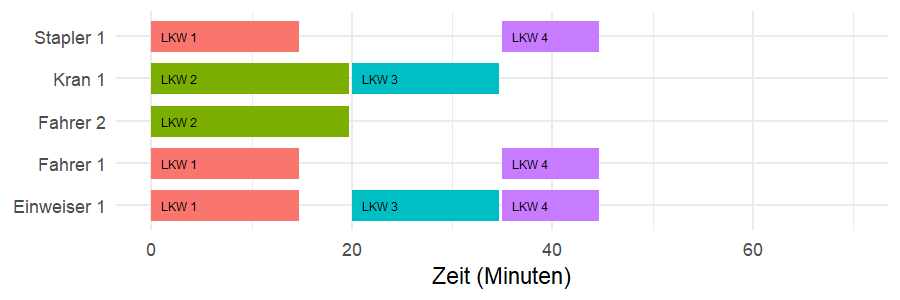
\includegraphics[width=\textwidth]{images/timelines/rsExampleSchedule.png}
    \caption{Beispielhafter Zeitplan für die Ressourcennutzung der Buchungen}
    \label{fig:rsExampleSchedule}
\end{figure}

Der Ansatz zur Umsetzung bzw. zur Lösung des beschriebenen Problems wäre es nun also, einen passenden Scheduling Algorithmus zu finden und möglicherweise leicht anzupassen. Dies stellte sich allerdings bei genauerer Recherche als gar nicht so einfach heraus, wie es im ersten Moment klingt. Es handelt sich hier schon um einen sehr speziellen Anwendungsfall mit einigen besonderen Anforderungen. Im folgenden werden einige genauer betrachtete Möglichkeiten erläutert, viele hatten allerdings gemeinsam, dass sie nur mit extremer Abwandlung des Algorithmus oder des Problems anwendbar wären. Dann hätte die darauf aufbauende Lösung allerdings kaum noch etwas mit dem eigentlichen Problem und Ziel dieser Arbeit zu tun.

\textbf{Job Shop Scheduling}
\todo{NP-schwer erwähnen?!}

Ein verbreitetes Optimierungsproblem, welches durchaus auch gewissen Ähnlichkeit zu dem hier dargestellten Problem hat, ist das Job-Shop Scheduling bzw. das Job-Shop Problem.

Ziel dieses Verfahrens ist es, eine Maschinenbelegung zu planen. Ein Beispiel für einen so optimierten Produktionsprozess ist in Abb. \ref{fig:job_shop_skizze} dargestellt. Jeder Job muss dabei nacheinander mehrere Maschinen belegen. Im Beispiel muss jedes Blatt Papier durch alle Druckmaschinen mit den Farben Grün, Blau und Gelb laufen. Dafür soll eine optimale Reihenfolge gefunden werden, wann welcher Job auf welcher Maschine bearbeitet wird, sodass die gesamte Produktionsdauer möglichst gering ist. Der Prozess kann aber auch komlexer sein. So können verschiedene Jobs unterschiedliche Maschinen benötigen. So sind in Varianten des JSP u.a. auch doppelte Maschinen oder eine feste Reihenfolge der Abarbeitung möglich. \cite{jobshop1}

\begin{figure}[H]
    \centering
    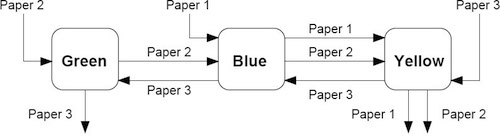
\includegraphics[width=0.8\textwidth]{images/jobshopdiagram.jpg}
    \caption{Beispielhafte Produktion zur Planung mit Job Shop Scheduling \cite{jobshop2}}
    \label{fig:job_shop_skizze}
\end{figure}

Ein daraus resultierender Zeitplan ist beispielhaft in Abb. \ref{fig:job_shop_schedule} zu erkennen. Für jede Maschine wurden hier ein Zeitfenster bestimmt, wann sie für welchen Job arbeitet. Dadurch das die Bearbeitungszeiten sehr große Unterschiede haben können, ist eine gute Verteilung wichtig, damit sich möglichst wenige Jobs gegenseitig blockieren und die Gesamtzeit des Plans verkürzt werden kann.

\begin{figure}[H]
    \centering
    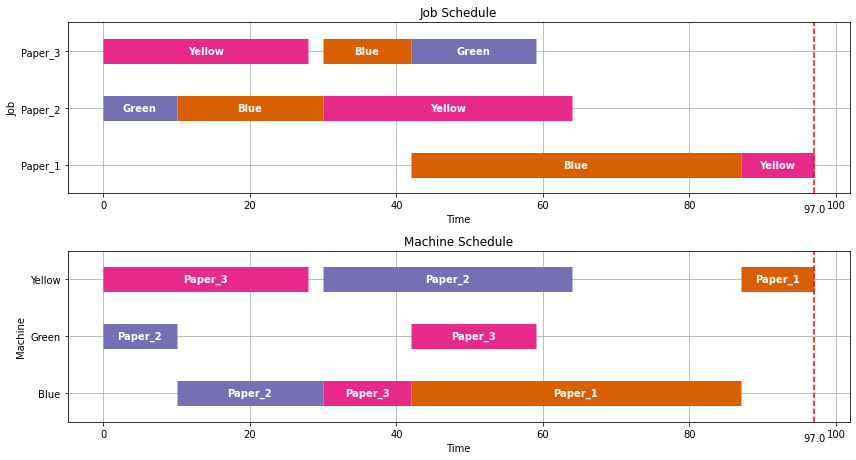
\includegraphics[width=\textwidth]{images/jobshopdiagram_schedule.png}
    \caption{Mittels Job-Shop-Verfahren ermittelter Zeitplan der Produktion \cite{jobshop2}}
    \label{fig:job_shop_schedule}
\end{figure}

Der große Vorteil bei der Nutzung des Job Shop Problems (JSP) wäre, dass zum einen die Modellierung sehr standardisiert und somit einfach machbar ist. Zum anderen gibt es auch bereits diverse Libraries für die gängisten Programmiersprachen (bspw. für Python siehe \cite{jobshop2}). Dies macht auch die Umsetzung sehr einfach, da weniger Eigenarbeit nötig ist und auch alle Funktionen bereits vielfach getestet worden sein dürften.

Prinzipiell ist dieser Ansatz deswegen ein sehr vielversprechendes Verfahren. Würde man die im Terminal verfügbaren Ressourcen und Ladehilfsmittel als Maschinen im Sinne des Job-Shop Problems sehen und jeden LKW als Job, welcher durch bestimmt Ressourcen abgearbeitet werden muss, du klingt dies durchaus passend. Auch die Art und Weise des resultierenden Zeitplans ist sicherlich eine sehr gute Darstellung, wie die Belegungszeiten verschiedener Ressourcen eingeteilt werden können. Das große Problem ist allerdings, dass das Job-Shop Verfahren davon ausgeht, dass die Bearbeitung durch die Maschinen nacheinander erfolgt. In dem in dieser Arbeit vorliegenden Problem, müssen die Ressourcen aber immer zeitgleich belegt werden. Es wird beispielsweise immer ein Stapler mit Einweiser zusammen benötigt. Es macht hier keinen Sinn eine Palette zunächst abzuladen und später erst einen Einweiser zu holen. Auch Varianten des JSP bieten hier keine passende Grundlage. Eine entsprechende Abwandlung des Ausgangsproblems würde auch zu einer solch großen Veränderung führen, dass das Ergebnis dann noch mehr viel mit dem angestrebten Ziel dieser Arbeit zu tun hätte. Aus diesem Grund wurde der Ansatz zur Nutzung des JSP nicht weiter verfolgt.


\textbf{Constraint Programmierung}

Constraint Programmierung ist ein weiterer sehr interessanter Ansatz, um sich dem vorliegenden Problem zu nähern. Er bietet die Möglichkeit, kombinatorische Probleme zu lösen. Ziel dieses Verfahrens ist es, ein großen Problem, mit einer großen Menge von Lösungen so weit begrenzt, dass eine überschauberere Teilmenge herauskommt. Es gibt dabei Variablen und Einschränkungen (engl. constraints). Solche Constraints sind keine Schritte oder Anweisungen, wie man sie aus gewöhnlichen Programmiersprachen kennt, sondern eher Eigenschaften einer machbaren Lösung. Außerdem ist es möglich sogenannte \glqq{}Soft Constraints\grqq{}, also nicht zwingende, aber wünschenswerte Bedingungen hinzuzufügen. Ein allgemeiner Constraint Solver kann dann genutzt werden, um machbare Werte für die Variablen bzw. eine passende Lösungen zu finden. Es ist hier also neben der Spezifikation von Einschränkungen keine spezielle Programmierung nötig. Implementationen von Constraint Solvern gibt es in diversen Programmiersprachen. \cite{constraintProgramming}

Größtes Problem dieses Verfahrens ist es, dass es in seiner Basis eher um die Prüfung der Machbarkeit, also um das finden einer durchführbaren Lösung geht. Das Optimieren und finden der besten Lösung ist eine zusätzliche Erweiterung. \cite{constraintProgramming} Es gibt durchaus Möglichkeiten, das vorliegende Problemszenario umzusetzen und sicherlich auch eine Optimierung zu finden. Beispielsweise gibt es mit \glqq{}choco-solver\grqq{} \cite{chocoSolver} auch eine sehr gute Java Library. Allerdings erschien es in ersten, sehr kurzen Versuchen mit der Library nicht ganz so einfach, das hier gestellte Problem in Constraints zu erfassen. Sicherlich wäre dies zumindest mit einem grundlegenden Umfang durchaus machbar, allerdings erschien der Zeitaufwand nicht sehr hoch und die im Folgenden beschriebene Lösung vielversprechender, sodass dieses Konzept nach einer Recherche zurückgestellt und nicht weiter umgesetzt wurde.


\textbf{Lösung durch Heuristiken}
\todo{Überarbeiten?!}

Alle bisher betrachteten Verfahren sind eher klassische Optimierungsprobleme, welche für ein Ausgangsproblem mit vorgegebenen Wegen eine Lösung finden. Da diese Verfahren aber alle nicht gut für das hier gegebene Problem geeignet sind, erscheint es als gute und machbare Alternative, Heuristiken zu nutzen.

Heuristiken sind dabei Methoden, über ein analytisches Vorgehen und mit begrenztem Wissen, dennoch eine möglichst gute und zumindest annähernd optimale Lösung zu finden \todo{Quelle}. Auf das vorliegende Problem bezogen könnte man sich also überlegen, wie eine Sortierung der Buchungen vorgenommen werden könnte, sodass mehr Buchungen mit weniger Wartezeit eingeplant werden können, als dies unoptimiert der Fall ist. Klassische Prinzipien sind dabei z.B. \glqq{}Shortest Job Next\grqq{} oder \glqq{}Earlist Deadline First\grqq{}. \todo{Quelle}

Bei diesem Vorgehen ist die eigene Arbeit zur Implementierung höher, da es keine fertige Library gibt, die genau das gewünschte tut. Allerdings gibt es damit auch deutlich Flexibilität, was sehr gut ist, um den Algorithmus an die speziellen Anforderungen dieses Problems anzupassen.


\subsubsection{Algorithmus 2: Optimale Reihenfolge für Ladehilfsmittel}

Ein zweiter Weg, die man für das vorliegende Problem eine Optimierung erzielen könnte ist es, die Reihefolge bei der Bearbeitung der LKW so zu gestalten, dass Fahrtzeiten, Rüstzeiten u.ä. möglichst gering gehalten werden. Auch für diesen Fall ist eine gut und vollständige Avisierung essenziell. Ohne entsprechend gute Datenlage, ist es in keinem Fall denkbar eine gute Vorabplanung durchzuführen. Ist nämlich klar, welche LKW kommen, ist auch hier wieder gegeben, welche Ressourcen und Ladehilfsmittel benötigt werden. Wenn außerdem aus Erfahrungswerten bekannt ist, wie lang die Ladezeiten für bestimmte Güter mit den passenden Hilfmittel ist, wie lang Anfahrtzeiten oder Wechsel zwischen bestimmten Hilfsmitteln dauern, so kann eine relativ gute Schätzung abgegeben werden, wie lange es dauert, einen LKW nach einem beliebigen anderen abzuladen. Und genau hier wäre an dieser Stelle das Potenzial zur Optimierung. Durch gezieltes sortieren kann die Gesamtdauer der Bearbeitung reduziert werden. Mussten im unoptimierten Fall z.B. ein LKW per Stapler, dann einer per Kran und danach wieder einer per Stapler abgeladen werden, so musste der Stapler extra wieder wegfahren und hatte zusätzlich Leerlaufzeiten. Im optimierten Fall könnten solche Aufträge direkt nacheinander bearbeitet werden. Muss vielleicht auch nur ein Anbauteil getauscht werden, um weitere Aufträge zu erledigen, so kann dies auch schneller gemacht werden, wenn das entsprechende Fahrzeug ohnehin bereits am Ladeplatz ist.

Die Idee zur Lösung wäre hier, einen Algorithmus zu finden, welcher eben genau dieser Sortierung vornehmen kann. Im einfachsten Fall könnte man dies für einen Ladeplatz machen. Etwas komplexer wird das Problem, wenn zusätzliche Ladeplätze hinzukommen. Hier wird die Herausforderung, gleichzeitig eine möglichst optimale Zuordnung zu den entsprechenden Plätzen zu ermitteln und gleichzeitig innerhalb jedes Platzes die beste Sortierung beizubehalten. Insgesamt ist dieses Szenario ein Problem der kombinatorischen Optimierung\todo{Quelle?}. Zur Lösung dieses speziellen Falls bleiben gar nicht mehr so viele Optionen übrig und es lässt sich sehr schnell ein gut geeignetes Verfahren finden.

\textbf{Lösung durch Heuristiken}
\todo{Gut? Heuristiken werden auch bei TSP genutzt...}

Was man an dieser Stelle natürlich auch wieder versuchen könnte, wäre mit Heuristiken zu arbeiten. Wie in vielen praxisnahen Anwendungsfällen, lassen sich über Erfahrungswerte sicherlich gute und praxistaugliche Ergebnisse erzielen. So könnte man sicherlich mit einer guten Datenbasis ermitteln, welche Waren sich gut nacheinander abladen lassen und so in der Reihenfolge kombiniert werden können. Allerdings wird dabei auch immer eine relativ große Unsicherheit vorhanden sein, was die Effektivität dieses Verfahrens angeht, da Heuristiken selten das best mögliche Ergebnis erzielen.

\textbf{Anwendung des Traveling Salesman Problems}

Welche Lösung sich in diesem Fall dagegen sehr aufdrängt, ist die Nutzung des Traveling Salesman Problems (für Grundlagen siehe Kapitel \ref{sec:grundlagen_tsp}). Schaut man sich typische Probleme der kombinatorischen Optimierung an, so stellt man schnell fest, dass sich das Ausgangsproblem des TSP sehr gut auf das hier vorliegende Problem übertragen lässt. Sieht man die abzufertigenden LKWs als Knoten eines Graphen, so könnte der Aufwand bzw. die Kosten eines LKW, der nach einem Anderen abgefertigt werden soll, auf den Kanten dargestellt werden. So lässt sich ein vollständiger, gerichteter Graph aufstellen, also ein Graph welcher zwischen allen Knoten zwei Kanten, jeweils eine in jede Richtung hat \cite{graphenEckenKanten}. Auch die Umsetzung für mehrere Ladestellen lässt sich in der Theorie gar nicht so kompliziert lösen. Die Überlegung ist hier, das multiple Traveling Salesmen Problem zur Hilfe zu nehmen. Die Handelsreisenden stehen dabei für die Ladeplätz, bzw. deren Personal, Maschinen und Ressourcen. Mit dem normalen TSP lässt sich ein Ladeplatz bedienen. Durch Anwendung des mTSP lässt sich die gleiche Ausgangslage, also gleiche Buchungen und gleicher Graph mit mehreren Handelsreisenden bedienen. Es ergibt sich der beste Weg, mit mehreren Abladeeinheiten, d.h. auch eine parallele Bearbeitung ist zu möglich.

Das erste Teilproblem bei der Implementierung wäre es dann, eine möglichst gute Kostenberechnung zu machen. Will man nun z.B. die Kosten zum Abladen von LKW Y nach LKW X haben, müsste man eben bedenken, ob für beide das gleiche Geräte gebraucht wird, dann reicht es möglicherweise nur die Abladezeit von LKW von LKW Y zu berücksichtigen. Bedarf es einem Gerätewechsel, so müssten zusätzlich die Abrüstzeiten der Ladehilfsmittel von LKW X und die Aufrüstzeiten der neuen Ladehilfsmittel einbezogen werden. Der zweite Aspekt zur Umsetzung dieses Ansatzes ist das eigentliche Lösen des TSP, also im Endeffekt das finden des kürzesten Weges durch den zuvor aufgestellten Graphen. Hier gibt es auch bereits fertige Algorithmen zur Lösung. Entweder über passende Libraries oder durch manuelle Implementierung kann so durch das Programm eine optimierte Lösung gefunden werden. Abzuwägen ist hier, welcher Algorithmus gut funktioniert. Hier muss der beste Kompromiss zwischen Rechenzeit und Qualität der Lösung gefunden werden. Es ist zu vermuten, dass exakte Algorithmen gerade mit steigender Zahl von LKW ihre Probleme haben werden, sodass hier untersucht werden muss, wie genau die Lösungen heuristischer Verfahren sind.

Insgesamt sollte sich so aber von der Erzeugung eines passenden Graphen aus einer Liste von eingegebenen Avisierungen und einer anschließenden Lösung durch entsprechende Verfahren, ein geeigneter Algorithmus zur Planung der Reihenfolge der LKW entwickeln lassen.

\subsection{Konzeption Algorithmus 1}

Nach der Abwägung von geeigneten Optionen zur Lösung des Problems, folgt nun die konkrete Planung, wie diese Ansätze softwaretechnisch umgesetzt werden können.

Ziel des ersten Prototypen soll es sein, einen Algorithmus zu entwickeln, welcher die benötigten Ressourcen aus einer Menge von avisierten LKW möglichst gut auf die zur Verfügung stehenden aufteilt. Die Implementierung soll dabei in Java erfolgen. Dabei soll in erster Linie der Algorithmus umgesetzt werden und als Proof of Concept zeigen, dass er funktioniert. Dazu reicht es aus, wenn der Algorithmus, bzw. implementierte Varianten als JUnit Tests lauffähig sind. Eine Benutzeroberfläche o.ä. sollen also zum jetzigen Zeitpunkt nicht implementiert werden.

\subsubsection{Klassen und Datenstrukturen}

\subsubsection{Umsetzung} \todo{Erklären: Warum erscheint welches Verfahren sinnvoll (bevor es im praktischen Test ausprobiert wurde)}

Kern der Umsetzung wird es sein, Zeitplanobjekte zu erzeugen. Es muss eine Liste von Zeitplänen geben, für jede Ressource einen. Ein entsprechender Algorithmus muss dann aus der Liste von avisierten LKW jeweils Zeitfenster ermitteln, die jeder Auftrag zum Abarbeiten benötigt. Dabei ist zum einen die Dauer der Abfertigung entscheidend. Diese sollte sich aus den jeweiligen Aufträgen ermitteln lassen. Um eine gute Abschätzung zu erhalten, soll hier als Näherung die Abladezeit pro Gut verwendet werden. Diese soll später aus Erfahrungswerten für jedes Fahrzeug gesetzt werden. Zusätzlich muss aus einer vollständigen Avisierung hervor gehen, welcher HandlingCategory diese angehört. Danach ist genau festgelegt, welche Kategorie welche Ladehilfsmittel und Ressourcen belegt.

Da nun eindeutig klar ist, welche Buchung welche Ressourcen für wie viel Zeit belegt, muss es nun entsprechender Algorithmus entwickelt werden, welcher eine optimale Verteilung auf die verfügbaren Ressourcen vornimmt. Ziel sollte es dabei sein, möglichst wenig Leerlauf der Ressourcen zu haben und die Aufträge so eng wie möglich einzuordnen, dass möglichst viele davon in einem Zeitslot Platz finden. Wie bereits diskutiert, erscheint es hier die beste Lösung zu sein, diese Verteilung auf Basis von Heuristiken vorzunehmen. Es soll also eine systematische Verteilung auf Basis von Erfahrungswerten erfolgen. Da es in der theoretischen Planung sehr schwer ist, abzuschätzen, wie sich ein bestimmtes System in der Praxis verhält, sollen hier die am vielversprechendsten klingenden Konzepte erläutert werden. Im Anschluss sollen diese dann alle implementiert werden. Über entsprechende Tests kann dann verglichen werden, wie viel Verbesserung sich dadurch erzielen lässt, bzw. bei welchen Teilaspekten sich welches System am besten verhält. U.a. kann hier die Zahl der abgefertigten LKW pro Slot verglichen werden, denkbar sind z.B. aber auch Leerlaufzeiten der Ressourcen oder die Performance des jeweiligen Algorithmus.

\todo{Grunsätzliches System zur einordnung in den Zeitplan erklären, also next possible window etc?}


Nachfolgend sollen einmal alle denkbaren Verfahren zur Sortierung des Zeitplans beschrieben werden. Dafür wird die beispielhafte Liste der Avisierungen aus Tabelle \ref{tab:exampleAdvices} verwendet und jeweils gezeigt, wie nach die Sortierung nach diesen Verfahren auf einen gleichbleibende Menge von Ressourcen aussehen würde. Die jeweiligen Verfahren wurden dabei aus der genaueren Betrachtung der Anforderungen bzw. aus möglichen Optimierungszielen ermittelt.

\begin{table}[!h]
\begin{center}
\caption{Beispielhafte Liste von LKW Avisierungen für einen Slot}
\label{tab:exampleAdvices}
\begin{tabular}{c|c|c} 
    LKW & benötigte Ressourcen & Dauer (min) \\\hline
    1 & Stapler, Fahrer, Einweiser & 12 \\\hline
    2 & Kran, Einweiser & 15 \\\hline
    3 & Fahrer, Einweiser & 5 \\\hline
    4 & Fahrer, Einweiser & 5 \\\hline
    5 & Reachstacker, Fahrer & 8 \\
\end{tabular}
\end{center}
\end{table}

\textbf{Smallest window next (smallest job next?!)} \todo{SJN erklären}

Ein erstes Verfahren, welches sinnvoll erscheint, ist die Verteilung der Aufträge nach dem \glqq{}Shortest Jobs Next\grqq{}-Prinzip. Hierbei würde für jeden LKW die Bearbeitungsdauer ermittelt werden und jeweils nacheinander die LKW von der kleinsten zur größten Dauer an den nächsten jeweils passenden Zeitpunkt wo alle benötigten Ressourcen frei sind, einsortiert werden. Eine beispielhafte Verteilung der LKW ist in Abbildung \ref{fig:rsSjnExample} dargestellt. Der Vorteil, weshalb dieses Verfahren vor allem sinnvoll erscheint, ist, so schnell möglichst viele LKW abgearbeitet werden. Alle Aufträge, welche schnell zu erledigen sind, werden direkt abgearbeitet und die potenzielle Wartezeit der LKW Fahrer minimiert.

\begin{figure}[H]
    \centering
    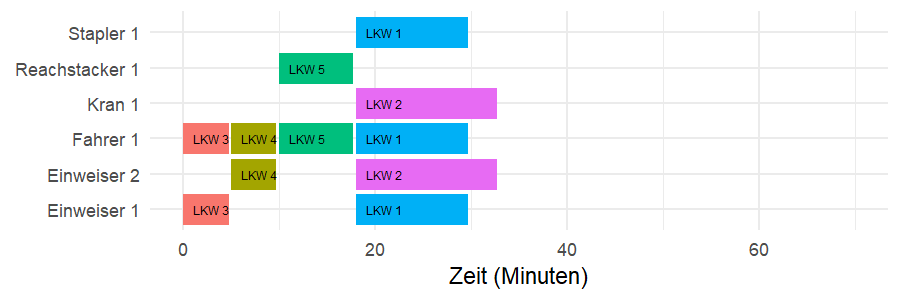
\includegraphics[width=\textwidth]{images/timelines/rsShortestJobNextExample.png}
    \caption{Planung der LKW aus Tabelle \ref{tab:exampleAdvices} nach dem Shortest Job Next Prinzip}
    \label{fig:rsSjnExample}
\end{figure}

Für das gezeigte Beispiel würde das bedeuten, dass diese nach ihrer Bearbeitungsdauer sortiert bearbeitet werden. Zunächst LKW 3 und danach LKW 4, da diese beide den Fahrer brauchen und so nicht parallel arbeiten können. LKW 5 kommt anschließend und braucht ebenfalls einen Fahrer. LKW 1 würde dann verplant werden, kann aber parallel zu LKW 2 laufen, da hier keine überschneidenden Ressourcen benötigt werden, bzw. es zwei Einweiser gibt.


\textbf{Biggest window next (smallest/biggest job next?!)}

\textbf{Most idle time next}

Ein Hauptziel der Optimierung ist die Reduzierung der Leerlaufzeiten und dadurch eine schnellere und effizientere Abarbeitung der Aufgaben. Eine weitere Idee, um eine möglichst gleichmäßige Auslastung der Ressourcen zu erreichen, wäre es also, immer den Auftrag als nächstes einzuplanen, der die Ressource mit der bis dahin größten Leerlaufzeit benötigt.

\begin{figure}[H]
    \centering
    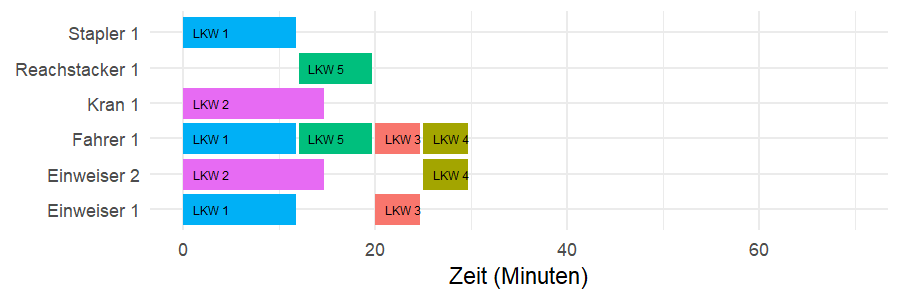
\includegraphics[width=\textwidth]{images/timelines/rsMostIdleExample.png}
    \caption{Planung der LKW aus Tabelle \ref{tab:exampleAdvices} nach dem Most idle time next Prinzip}
    \label{fig:rsMitnExample}
\end{figure}

Für das vorliegende Beispiel  (Abb. \ref{fig:rsMitnExample}) würde dies folgendes bedeuten: Für den Beginn könnte man nach dem first come, first served Prinzip arbeiten, da sind eben alle Ressourcen noch frei. Anschließend sind Kran und Einweiser noch ganz frei, sodass LKW 2 als nächstes kommen würde. Das gleiche gilt danach für den Reachstacker und LKW 5 und schlussendlich wären dann die Einweiser am wenigsten belegt, sodass LKW 4 und LKW 5 anschließend abgeladen werden.

\textbf{First come, first served}

Ein letztes Konzept, welches kein so systematisches Prinzip hat, wäre das die Abarbeitung in der Reihenfolge ihrer Buchung bzw. in einer zufälligen Reihenfolge. Idee könnte hier sein, dass sich dadurch Ungleichheiten ausgleichen und durch die Zufallskomponente eine gut durchmischte und gleichmäßige Verteilung entsteht. Bei den anderen Verfahren, insbesondere \glqq{}Shortest Job Next\grqq{} wäre zu untersuchen, wie gut und gleichmäßig die Verteilung nach solchen Prinzipien wird. Möglicherweise könnten sich Probleme ergeben, dass LKWs gleicher Ladekategorie tendenziell immer kürzer sind und somit viele Ressourcen eines Typs ausgelastet werden, während andere viel Leerlauf behalten.

\begin{figure}[H]
    \centering
    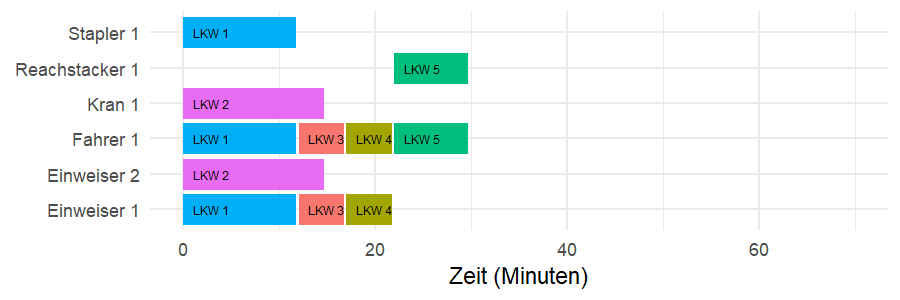
\includegraphics[width=\textwidth]{images/timelines/rsFcfsExample.png}
    \caption{Planung der LKW aus Tabelle \ref{tab:exampleAdvices} nach dem Fist come, first served Prinzip}
    \label{fig:rsFcfsExample}
\end{figure}

Für das hier gezeigte Beispiel (Abb. \ref{fig:rsFcfsExample}) würde dies bedeuten, dass LKW 1 und LKW 2 parallel laufen können und somit schon eine gute Auslastung der Ressourcen in der ersten Zeit ergeben. LKW 3, 4 und 5 müssten dann nacheinander abgearbeitet werden, da alle einen Fahrer benötigen.



\todo{Weitere Verfahren?}

\subsubsection{Vergleichswerte zur Auswertung generieren}

Um eine gute Bewertung der zuvor geplanten Sortierungsverfahren anstellen zu können, wäre es von Vorteil, Daten als Ausgangszustand zu haben. Da es allerdings kaum Datensätze gibt, die darstellen würde, wie LKW aktuell Verteilt werden, wäre die Idee an dieser Stelle, zusätzlich ein Verfahren zu entwickelt, welches den Zeitplan so erzeugen kann, wie es vermutlich im aktuellen und nicht optimierten Zustand erfolgen würde. Dann ließen sich Vorher-Nachher Vergleiche ziehen und eine genauere Bewertung vornehmen.

Ausgangspunkte, wie eine solche Sortierung aussehen würde, wäre, dass LKW innerhalb ihres gebuchten Slots kommen, wann sie wollen, d.h. aus Hafensicht gesehen in zufälliger Reihenfolge. Die Abarbeitung würde also nach dem \glqq{}first come, first served\grqq{} Prinzip erfolgen. Erschwerend kommt allerdings noch hinzu, dass die LKW wie erwähnt nicht alle direkt bereit stehen, sondern zusätzlich noch zu einem aus Hafensicht zufälligen Zeitpunkt erscheinen, wodurch eine sehr lückenhafte Verteilung mit vielen Leerlaufzeiten der Ressourcen entsteht. Um dieses Sachverhalt zu implementieren wäre es also die Idee, sowohl die Reihenfolge der LKW Avisierungen, als auch jeweils einen Ankunftszeitpunkt innerhalb des Slots zufällig zu bestimmen. Anschließend kann jeder LKW zu seinen benötigten Ressourcen zugeteilt werden, entweder sobald er ankommt oder spätestens, wenn alle von ihm benötigten Ressourcen verfügbar sind. 


\subsection{Konzeption Algorithmus 2}

Wie auch schon Variante 1, soll auch dieser Prototyp in Java umgesetzt werden. Auch hier geht es hauptsächlich darum, die Algorithmen und Hintergrundlogik zu implementieren und weniger darum, schöne Benutzeroberflächen für direkte Benutzerein- und ausgaben zu schaffen. Auch die Erfassung der Daten von Fahrern und Speditionen soll nicht Teil er Implementierung sein, also auch nicht die Sammlung von Avisierungen für die Slots o.ä. Stattdessen erfolgt der Aufruf der Algorithmen über JUnit Testfälle. Hier soll mit gezielten oder generierten Eingabedaten gearbeitet werden und damit die Optimierung entsprechend durchgeführt werden.

\subsubsection{Klassen und Datenstrukturen}

\textbf{TruckAdvice}: Alle vom LKW Fahrer bzw. von der Spedition bei der Avisierung zu erfassenden Daten
\begin{itemize}
  \item goodType
  \item numberOfGoods
  \item description
  \item handlingCategory
  \todo{Länge, Breite, Höhe, Gewicht, ...?}
\end{itemize}

\textbf{GoodType}

\textbf{GoodType}

\textbf{HandlingCategory}

\textbf{HandlingMachines}


\subsubsection{Umsetzung}

Der das grundsätzliche Verfahren, nachdem eine Liste aller Avisierungen (TruckAdvice-Objekte) erfasst wurde ist in Abbildung \ref{fig:flowchart_tsp_algorithm} dargestellt.

\begin{figure}[H]
    \centering
    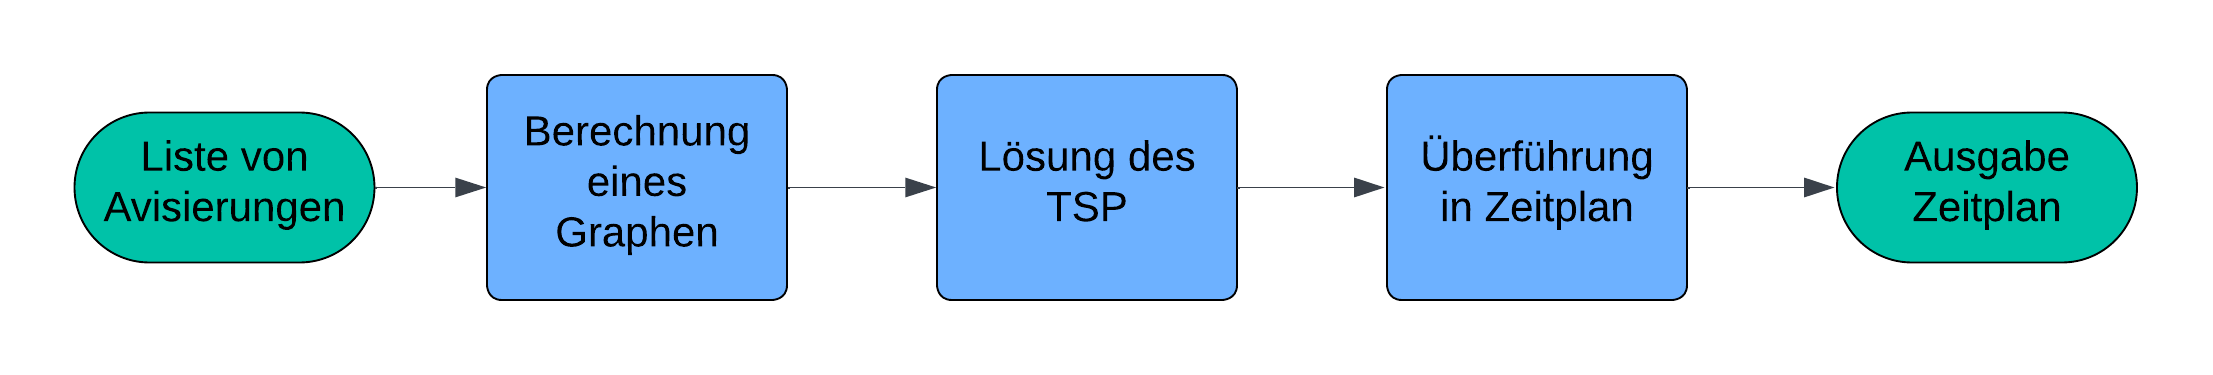
\includegraphics[width=\textwidth]{images/Flowchart TSP Algorithm.png}
    \caption{Ablaufdiagramm der Lösung mittels TSP}
    \label{fig:flowchart_tsp_algorithm}
\end{figure}

\subsubsection{Berechnung eines Graphen}

Zunächst einmal kann aus den gegebenen Daten ein vollständiger, gerichteter Graph erzeugt werden, bzw. in der Implementierung kann dieser als zweidimentionale Matrix dargestellt werde. Dabei ist jeder Knoten ein Auftrag aus der eingegebenen Liste. Für die Kanten wird eine Methode benötigt, die die Kosten bzw. Aufwände berechnen kann, welche benötigt werden, um einen beliebigen LKW nach einem Anderen abzufertigen. Um eine vergleichbare Einheit zu haben, wird hier immer mit Zeit in Minuten gearbeitet. Aus der bei der Datenerfassung ermittelten \textit{HandlingCategory} kann jeweils bestimmt werden, welche Ladehilfsmittel (HandlingMachines) und Ressourcen benötigt werden. Zu jedem Hilfsmittel sind in dem System entsprechende Zeiten hinterlegt. Für das hier zu erstellende Proof of Concept sollen das zunächst Anfahrt/Aufbauzeit, Ladezeit pro Gut sowie Abbau/Abfahrtszeit sein \todo{Komplexere Kostenberechnung?!}. Denkbar wären hier allerdings auch deutlich komplexere Berechnungen und Einflussfaktoren. Beispielsweise unterschiedliche Wechselaufwände, je nachdem zu welcher Maschine gewechselt wird. Um die Komplexität an dieser Stelle nicht zu hoch werden zu lassen, werden die Kosten zum Abfertigen von LKW B nach LKW A nach folgendem Schema berechnet:

Gleiche Maschine für A und B?\\
$\rightarrow Zeit_{AB} = numberOfGoods_B * ZeitProGut_B$

Ist ein Wechsel der Maschine nötig?\\
$\rightarrow Zeit_{AB} = Abbauzeit_A + Aufbauzeit_B + numberOfGoods_B * ZeitProGut_B$

Ein so erzeugter Graph bzw. dessen interne Darstellung als Matrix könnten wie in den Abbildungen \ref{fig:example_tsp_graph} und \ref{fig:example_tsp_matrix} aussehen.

\begin{figure}[H]
\centering
\begin{minipage}{.6\textwidth}
  \centering
  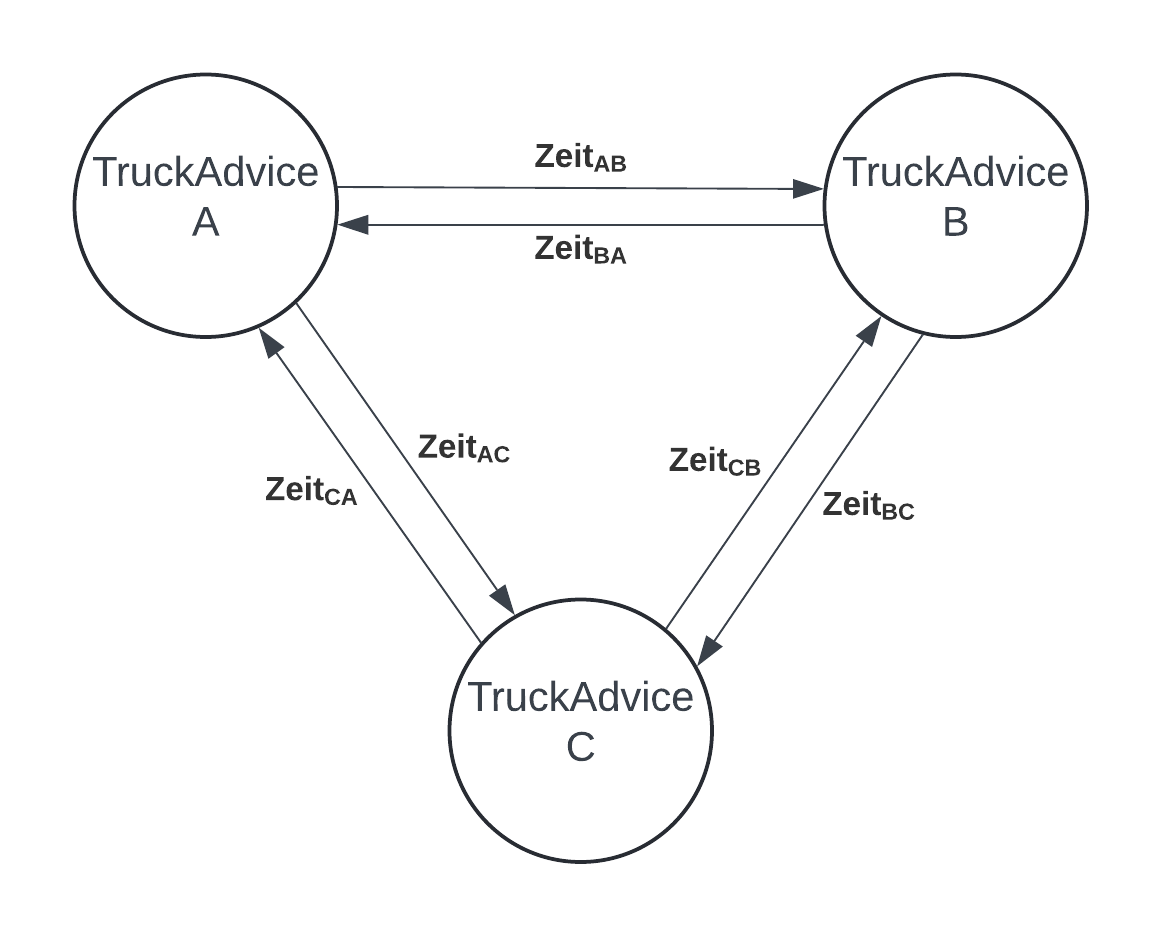
\includegraphics[width=\linewidth]{images/ExampleTSPGraph.png}
  \caption{Beispielhafte Darstellung von TruckAdvices mit Zeitaufwänden als Graph}
  \label{fig:example_tsp_graph}
\end{minipage}%
\begin{minipage}{.4\textwidth}
  \centering
    \[
    \begin{matrix}
         & A & B & C\\
        A & \infty & Zeit_{AB} & Zeit_{AC}\\
        B & Zeit_{BA} & \infty & Zeit_{BC}\\
        C & Zeit_{CA} & Zeit_{CB} & \infty
    \end{matrix}
    \]
  \caption{Zu Abb. \ref{fig:example_tsp_graph} passende Matrix}
  \label{fig:example_tsp_matrix}
\end{minipage}
\end{figure}
\todo{Matrix als Abb bezeichnen ok? evtl ändern...}









\subsubsection{TSP Lösungsverfahren}
\label{sec:tspVerfahrenPlanung}
\todo{Problem: Sehr unterschiedlich lange Zeit je Slot erwähnen und Lösung beschreiben}

Der zweite und wesentliche Schritt zur Optimierung ist nun die Lösung des TSP, also das finden eines möglichst kurzen Weges durch den zuvor erzeugten Graphen. Mit Blick auf das zu erzielende Ergebnis, fällt auf, dass das nach dem standardmäßigen TSP für einen Handlungsreisenden eine Kette von Stationen erzeugt würde. Übertragen auf das vorliegende Problem heißt das, dass aus allen Buchungen ein Zeitplan für einen einzigen Ladeplatz erzeugt wird. Dies ist zunächst auch ein gutes Zwischenergebnis und erfüllt schon einmal viele zuvor gesetzte Anforderungen. Um allerdings eine praxisnäheres Szenario abzubilden, wäre die Erweiterung auf mehrere Ladeplätze ein nicht ganz uninteressanter Punkt, um diesen hier bei der Planung ebenfalls umzusetzen. Dies ist bei genauerer Auseinandersetzung mit dem TSP und dessen Varianten auf den ersten Blick kein allzu großes Problem mehr. Für diesen Anwendungsfall dürfte nämlich das mTSP geeignet sein \cite{mtsp}. Hier werden statt einem Handlungsreisenden mehrere auf das gleiche Szenario angesetzt, die dann die Stationen unter sich aufteilen und parallel abarbeiten können. Dadurch ist die Vorarbeit die selbe, nur über die Anzahl von Handlungsreisenden kann nun entschieden werden, für wie viele Ladeplätze die Optimierung erfolgen soll.

Rein aus dieser theoretischen Sicht ist das TSP bzw. mTSP gar nicht so schwer zu verstehen und auf das vorliegende Problem zu übertragen. Für die Implementierung und somit den haupt Lösungsschritt aus dem Ablaufdiagramm (Abb. \ref{fig:flowchart_tsp_algorithm}), müssen nun allerdings passende Lösungsverfahren gefunden werden. Hier lassen sich für das normale TSP auch noch überschaubare Verfahren finden. Sehr viel komplizierter wird es bei der Lösung des mTSP. Hier sind die Verfahren sehr viel komplexer und schwieriger. Nach einiger Recherche als noch überschaubar und vom Aufwand her umsetzbar hat sich die Überführung von mTSP in normale TSP dargestellt. Dies hat den sehr großen Vorteil, dass zur Findung des besten Weges anschließend die ganz normalen, bekannteren und einfacheren Verfahren zur Lösung von TSP genutzt werden können. \cite{mtsp, mtspAlgosAndTransform}

\todo[inline]{Exkurs Transformation von mTSP zu TSP, wohin?}


Aus Softwaresicht muss nun also ein passendes Verfahren zur Lösung des TSP implementiert werden. Da Quellen mit passenden Implementierungen gefunden wurden, soll eine manuelle Implementierung, ohne Libraries erfolgen. Gleichzeitig lässt sich so eine bessere Kontrolle und Anpassbarkeit auf das vorliegende Problem erzielen und auch die Verfahren sind so besser verständlich. \todo{Evtl. auch nochmal mit Library probieren?} Da es einige verschiedene Algorithmen und Ansätze zur Lösung gibt, sollen hier mehrere implementiert werden, um diese anschließend zu vergleichen. Die nachfolgende Auswahl besteht dabei aus den bekanntesten Methoden und solchen, bei denen das Verhältnis zwischen Aufwand der Implementierung und Qualität des Ergebnisses am besten erschienen.

\textbf{brute-force Methode}

Zum einen sollen hier exakte Verfahren betrachtet werden. Der ineffizienteste und aufwändigste Weg, wäre die \textit{brute-force Methode}, d.h. alle möglichen Lösungswege durchgehen, deren Länge berechnen und immer wieder schauen, ob ein kürzerer gefunden wurde. Die Implementierung wäre vermutlich nicht allzu kompliziert, allerdings wird diese Methode sehr schnell an ihre Leistungsgrenze kommen. Da es hier wirklich offensichtlich bessere Ansätze gibt, wird dieser Weg aber nicht verfolgt. \cite{oracleTsp}

\textbf{Branch and Bound}
\todo{Beschreibung/Erklärung in Quelle \cite{constraintProgramming}, Seriöse Quellen hinzufügen, evtl. erweitern und überarbeiten}

Besser geeignet erscheint dagegen das Branch-and-Bound Verfahren. Von der Grundidee ist dieses sehr ähnlich zum brute-forcing, allerdings wird hier der kürzest mögliche Weg berechnet. Anschließend können dann per Ausschlussverfahren schon frühzeitig einige längere Wege ausgeschlossen werden, sodass der Gesamtaufwand der Berechnung verkürzt wird. \cite{travelingSalesman}

Das Prinzip dabei ist es, für jeden betrachteten Knoten eine \glqq{}Bound\grqq{}, also Grenze für einen Wert für die bestmögliche Lösung beim Weiterverfolgen der angrenzenden Knoten. Anhand dessen kann dann beim durchgehen der Äste und Möglichkeiten des Graphen entschieden werden, ob es sich im Vergleich zur insgesamt besten Lösung lohnt, die vorliegende Option weiter zu verfolgen oder ob diese bereits jetzt zu teuer ist und verworfen werden kann. Die minimalen Kosten können dabei berechnet werden, indem von allen Knoten die Kosten der kleinsten Kante und die der zweitkleinsten Kante summiert werden und das Gesamtergebnis halbiert wird. Die Halbierung wird vorgenommen, da jede Kante zweimal vorkommt. \cite{geeksForGeeksBnB}

\textbf{Reduced Matrix}
\todo{Bessere Quellen hinzufügen, Erklärungen Überarbeiten?}

Ein weiteres interessantes und exaktes Verfahren ist die Reduced-Matrix Methode. Diese ähnelt sehr dem Prinzip der Branch and Bound Methode, hierbei wird die optimale Lösung allerdings rechnerisch über die Umformung von Matrizen ermittelt. 

Das Prinzip hier ist es, dass die Zeilen und Spalten der Kostenmatrix reduziert werden können. Es wird dafür Zeile für Zeile und anschließend Spalte für Spalte durchgegangen. Enthalten diese jeweils keinen 0-Wert, so kann von allen Werten der jeweils kleinste abgezogen werden. Summiert man die Werte jeder Zeile und jeder Spalte, welche reduziert wurden, so ergiben sich die minimalen Kosten für diesen (Teil-)Graphen. \cite{geeksForGeeksRm}

\begin{figure}[H]
\centering
\begin{minipage}{.5\textwidth}
  \centering
  \[
    \begin{matrix}
          & 1 & 2 & 3 & 4\\
        1 & \infty & 10 & 15 & 20\\
        2 & 10 & \infty & 35 & 25\\
        3 & 15 & 35 & \infty & 30\\
        4 & 20 & 25 & 30 & \infty\\
    \end{matrix}
    \]
    \caption{Initiale Matrix \cite{geeksForGeeksRm}}
    \label{fig:reduced_matrix_initial}
\end{minipage}%
\begin{minipage}{.5\textwidth}
  \centering
   \[
    \begin{matrix}
          & 1 & 2 & 3 & 4\\
        1 & \infty & 0 & 5 & 10\\
        2 & 0 & \infty & 25 & 15\\
        3 & 0 & 20 & \infty & 15\\
        4 & 0 & 5 & 10 & \infty\\
    \end{matrix}
    \]
    \caption{Reduzierte Matrix aus Abb. \ref{fig:reduced_matrix_initial} \cite{geeksForGeeksRm}}
    \label{fig:reduced_matrix_reduced}
\end{minipage}
\end{figure}

Die Zeilen wurden jeweils um 10, 10, 15, 20 reduziert und die Spalten dann um 0, 0, 5, 10. So ergibt sich minimale Kosten für den gesamten Graphen von 10 + 10 + 15 + 20 + 5 + 10 = 70. Um im Baum fortzuschreiten kann die Matrix anschließend für jede Kante weiter reduziert werden. Um beispielsweise von Knoten 1 zu 2 zu kommen, werden die Werte der ersten Zeile und zweiten Spalte durch unendlich ersetzt und die Matrix erneut reduziert. 

\begin{figure}[H]
\centering
\begin{minipage}{.5\textwidth}
  \centering
  \[
    \begin{matrix}
          & 1 & 2 & 3 & 4\\
        1 & \infty & \infty & \infty & \infty\\
        2 & 10 & \infty & 35 & 25\\
        3 & 15 & \infty & \infty & 30\\
        4 & 20 & \infty & 30 & \infty\\
    \end{matrix}
    \]
    \caption{Matrix des Schritts von Knoten 1 zu Knoten 2 \cite{geeksForGeeksRm}}
    \label{fig:reduced_matrix_1-2}
\end{minipage}%
\begin{minipage}{.5\textwidth}
  \centering
   \[
    \begin{matrix}
          & 1 & 2 & 3 & 4\\
        1 & \infty & \infty & \infty & \infty\\
        2 & 0 & \infty & 10 & 0\\
        3 & 0 & \infty & \infty & 5\\
        4 & 0 & \infty & 0 & \infty\\
    \end{matrix}
    \]
    \caption{Reduzierte Matrix aus Abb. \ref{fig:reduced_matrix_1-2} \cite{geeksForGeeksRm}}
    \label{fig:reduced_matrix_1-2_reduced}
\end{minipage}
\end{figure}


Hier wird um 5, 0 und 0 bzw. um 0, 5 und 0 reduziert. Die Kosten der Reduktion von 10 können dann auf die zuvor ermittelten 70 addiert werden, um die minimalen Kosten im Baum zu erhalten.


So lässt sich aus dem beispielhaften Graphen (Abb. \ref{fig:reducedMatrixGraph}) im Endeffekt folgender Baum (Abb. \ref{fig:reducedMatrixTree}) bestimmt. Einige Äste mussten dabei nicht weiter verfolgt werden, da sie schon zum betrachteten Zeitpunkt nicht weniger Kosten würden als andere. Es zeigt sich, dass die Wege 1>3>4>2 und 1>2>4>3 die kürzesten sind. Zum Vorteil wird hier auch ausgenutzt, dass für das TSP immer geschlossene Pfade gesucht werden, d.h. hier ist es irrelevant mit welchem Knoten begonnen wird, es kann einfach mit einem beliebigen Knoten, in diesem Fall Knoten 1 gestartet werden. \cite{geeksForGeeksRm}

\begin{figure}[H]
\centering
\begin{minipage}{.4\textwidth}
  \centering

    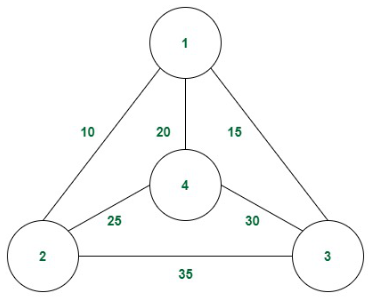
\includegraphics[width=\textwidth]{images/reducedMatrixGraph.png}
    \caption{Beispielhafter Graph}
    \label{fig:reducedMatrixGraph}

\end{minipage}%
\begin{minipage}{.6\textwidth}
  \centering
    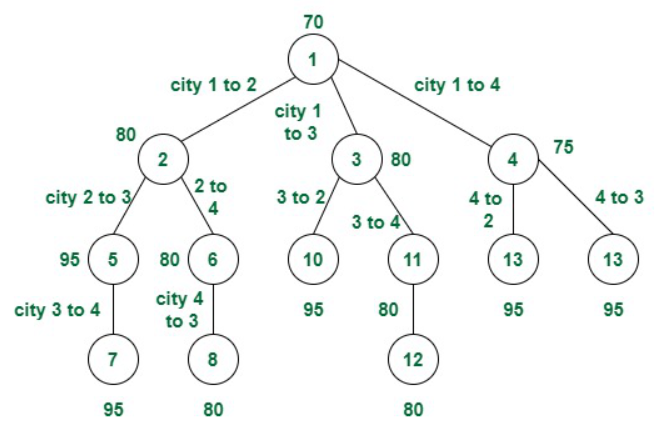
\includegraphics[width=\textwidth]{images/reducedMatrixTree.png}
    \caption{Alle mit der reduced Matrix Methode betracheteten Pfade}
    \label{fig:reducedMatrixTree}
\end{minipage}
\end{figure}


\textbf{Simulated Annealing}
\todo{Basiert auf: https://www.baeldung.com/java-simulated-annealing-for-traveling-salesman}

Ein weiterer Blick lohnt sich allerdings auch auf die heuristischen Verfahren. Im Gegensatz zu den zuvor beschriebenen, exakten Varianten, wird es hier nicht garantiert das beste Ergebnis geben. Allerdings wird es in den meisten Fällen dem besten Ergebnis sehr nahe kommen. Der große Vorteil könnte dafür allerdings sein, dass die Rechenzeit deutlich verringert wird. Dies könnte vor allem ein wichtiger Kompromiss sein, da die Größe der durch die anderen Verfahren lösbaren Graphen sehr begrenzt sein wird, gerade mit überschaubaren Rechenressourcen. Mit dem Simulated Annealing Ansatz sollte der Rechnenaufwand um ein vielfaches geringer sein und damit auch die Größe von möglichen Graphen deutlich steigen.

Ein bekanntes Verfahren ist hier das Simulated Annealing. Den Aufwand für jede Wegkombination im Graphen des TSP lässt kann man sich als kontinuierliche Funktion vorstellen. Ziel ist es dabei grundsätzlich das globale Optimum, also den kleines Wert über alle Möglichkeiten zu finden. Im Gegensatz zu den vorherigen Varianten, welche alle Möglichkeiten durchgehen, ist hier die Idee, sich dem besten Ergebnis durch ausprobieren bestimmter Möglichkeiten anzunähern. Dabei fängt man mit einer zufälligen Reihenfolge an. Nach jedem Versuch führt man kann man unterschiedliche, zufällige Operationen an der Reihenfolge durchführen, u.a. Tauschen von zwei Knoten, Verschieben eines Knotens. Auch die Nutzung von 2-Opt oder 3-Opt-Heuristiken ist denkbar. Hier werden zwei oder drei Kanten zwischen Knoten getrennt und untereinander neu verbunden, sodass sich einer neuer Pfad ergibt. Durch erneute Berechnung des Aufwand kann nun geschaut werden, ob sich das Ergebnis verbessert hat, dann wird dies als neuer Ausgangspunkt genutzt, andernfalls wird es verworfen. Durch Wiederholung dieses Vorgangs sollte sich das Ergebnis einem Optimum annähern. Es kann allerdings sein, dass dies ein lokales und kein globales Optimum ist. Hier kommt der eigentliche Trick des Simulated Annealings ins Spiel, es wird mit einer \glqq{}Temperatur\grqq{} gearbeitet. Durch eine exponentielle Funktion wird unter bestimmten Umständen doch das schlechtere Ergebnis gespeichert und die Möglichkeit geschaffen, aus dem lokalen Optimum auszubrechen. Durch senken der Temperatur im Verlauf der versuche wird diese Wahrscheinlichkeit geringer. Dieses Verfahren hat man sich von Abkühlungsprozesses aus der Natur abgeschaut. \cite{tspSimulatedAnnealing}

\begin{figure}[H]
    \centering
    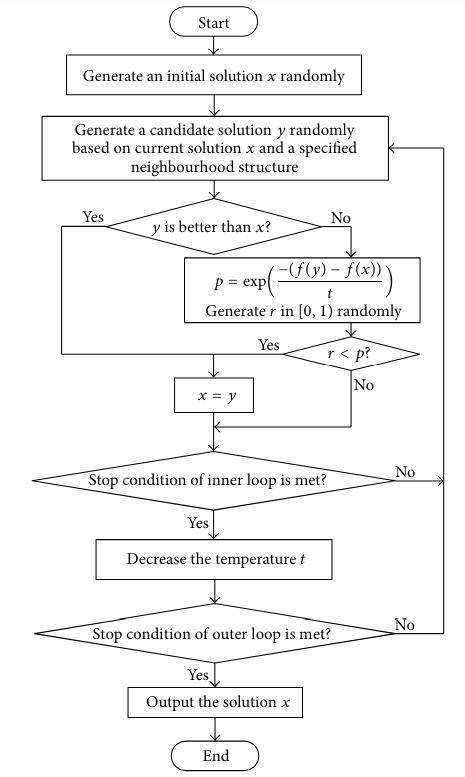
\includegraphics[width=0.6\textwidth]{images/flowSimulatedAnnealing.png}
    \caption{Ablauf von Simulated Annealing \cite{tspSimulatedAnnealing}}
    \label{fig:flowchart_simulated_annealing}
\end{figure}

Der Ablauf eines Simulated Annealing Prozesses ist in Abbildung \ref{fig:flowchart_simulated_annealing} dargestellt. Der Nachteil dieses Verfahrens ist, dass es mehrere Parameter gibt, die eingestellt werden müssen. So gibt es eine Maximalanzahl von Schleifendurchläufen, eine Starttemperatur und eine Abkühlungsrate. All diese Werte beeinflussen das Ergebnis. Komplexere Implementierungen können diese Werte selbst anpassen, eine manuelle Einstellung ist oft nicht so einfach und passiert eher nach dem \glqq{}trail and error\grqq{}-Prinzip. \cite{tspSimulatedAnnealing}

Insgesamt scheint die diese Variante zur Lösung allerdings vielversprechende Ergebnisse zu liefern und auch keine allzu komplexe Implementierung darzustellen.


\subsubsection{Transformation eines mTSP zu einem TSP}
\label{sec:mstpTransofrmation}

Um ein mTSP in ein einfaches TSP umzuwandeln, fügt man dem Graphen fiktive Knoten für die Startpunkte der Handlungsreisenden hinzu. Für ein beispielhaftes Problem aus n=9 Knoten und m=2 Handlungsreisenden fügt man m-1, also noch einen fiktiven Knoten hinzu. Ein Knoten wird ebenfalls fest als Startpunkt eines Handelsreisenden definiert. Das genannte Beispiel ist in Abbildung \ref{fig:mtsp_tranformation} zu sehen, wobei Knoten 1 der definierte Startpunkt und Knoten 10 der hinzugefügte, fiktive Knoten ist. Im Vergleich der Ausgangsmatrix (Abbildung \ref{fig:mtsp_distance_matrix}) und der erweiterten Maxtrix (Abbildung \ref{fig:mtsp_distance_matrix_with_dummys}) zu sehen ist, werden die Gewichte zwischen den Startpunkten sehr hoch gesetzt, wie es auch schon in der Diagonale zwischen Identischen Knoten der Fall ist, sodass kein Reisen direkt zwischen Startpunkten möglich ist. Ein Nachteil ist allerdings, dass die Größe des Graphen bzw. der Matrix ansteigt und dadurch der Lösungsaufwand erhöht wird, welcher mit steigender Zahl von Knoten ohnehin schon exponentiell steigt. \cite{mtsp, mtspTransform2}

\begin{figure}[H]
    \centering
    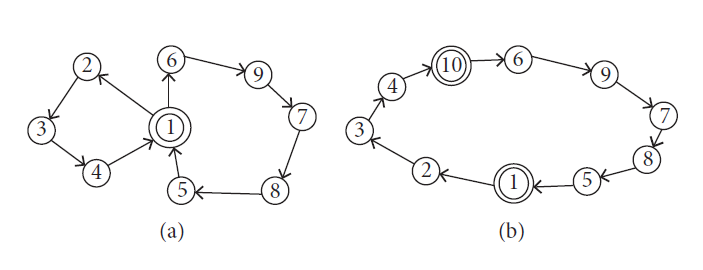
\includegraphics[width=\textwidth]{images/mtspTransformation.png}
    \caption{Lösung eines mTSP und Transformation zu TSP \cite{mtspTransform2}}
    \label{fig:mtsp_tranformation}
\end{figure}

\setcounter{MaxMatrixCols}{20}
\begin{figure}[H]
\centering
\begin{subfigure}{.44\textwidth}
  \centering
  \begin{footnotesize}
    \[
    \setlength{\arraycolsep}{0.1cm}
    \begin{matrix}
          & 1 & 2 & 3 & 4 & 5 & 6 & 7 & 8 & 9\\
        1 & 999 & 7 & 15 & 9 & 10 & 6 & 8 & 9 & 10\\
        2 & 11 & 999 & 8 & 7 & 11 & 3 & 6 & 4 & 3\\
        3 & 15 & 5 & 999 & 16 & 12 & 5 & 8 & 13 & 4\\
        4 & 2 & 5 & 11 & 999 & 9 & 13 & 14 & 4 & 2\\
        5 & 8 & 6 & 3 & 5 & 999 & 6 & 7 & 10 & 9\\
        6 & 6 & 13 & 8 & 11 & 5 & 999 & 5 & 4 & 5\\
        7 & 5 & 15 & 3 & 7 & 12 & 6 & 999 & 8 & 9\\
        8 & 9 & 3 & 9 & 14 & 3 & 11 & 8 & 999 & 10\\
        9 & 11 & 16 & 3 & 9 & 10 & 7 & 9 & 10 & 999\\
        &&&&&&&&&
    \end{matrix}
    \]
    \end{footnotesize}
  \caption{Distanzmatrix}
  \label{fig:mtspMatrix1}
\end{subfigure}
\begin{subfigure}{.54\textwidth}
  \centering
  \begin{footnotesize}
  \[
  \setlength{\arraycolsep}{0.1cm}
    \begin{matrix}
          & 1 & 2 & 3 & 4 & 5 & 6 & 7 & 8 & 9 & 10\\
        1 & 999 & 7 & 15 & 9 & 10 & 6 & 8 & 9 & 10 & 999\\
        2 & 11 & 999 & 8 & 7 & 11 & 3 & 6 & 4 & 3 & 11\\
        3 & 15 & 5 & 999 & 16 & 12 & 5 & 8 & 13 & 4 & 15\\
        4 & 2 & 5 & 11 & 999 & 9 & 13 & 14 & 4 & 2 & 2\\
        5 & 8 & 6 & 3 & 5 & 999 & 6 & 7 & 10 & 9 & 8\\
        6 & 6 & 13 & 8 & 11 & 5 & 999 & 5 & 4 & 5 & 6\\
        7 & 5 & 15 & 3 & 7 & 12 & 6 & 999 & 8 & 9 & 5\\
        8 & 9 & 3 & 9 & 14 & 3 & 11 & 8 & 999 & 10 & 9\\
        9 & 11 & 16 & 3 & 9 & 10 & 7 & 9 & 10 & 999 & 11\\
        10 & 999 & 7 & 15 & 9 & 10 & 6 & 8 & 9 & 10 & 999\\
    \end{matrix}
    \]
    \end{footnotesize}
  \caption{Erweiterte Distanzmatrix}
  \label{fig:mtspMatrix2}
\end{subfigure}

\caption{Distanzmatrixen zum Beispiel in Abb. \ref{fig:mtsp_tranformation} \cite{mtspTransform2}}
\label{fig:mtspMatricies}
\end{figure}

\begin{comment}

\begin{figure}[H]
    \centering
    \begin{small}
    \[
    \begin{matrix}
          & 1 & 2 & 3 & 4 & 5 & 6 & 7 & 8 & 9\\
        1 & 999 & 7 & 15 & 9 & 10 & 6 & 8 & 9 & 10\\
        2 & 11 & 999 & 8 & 7 & 11 & 3 & 6 & 4 & 3\\
        3 & 15 & 5 & 999 & 16 & 12 & 5 & 8 & 13 & 4\\
        4 & 2 & 5 & 11 & 999 & 9 & 13 & 14 & 4 & 2\\
        5 & 8 & 6 & 3 & 5 & 999 & 6 & 7 & 10 & 9\\
        6 & 6 & 13 & 8 & 11 & 5 & 999 & 5 & 4 & 5\\
        7 & 5 & 15 & 3 & 7 & 12 & 6 & 999 & 8 & 9\\
        8 & 9 & 3 & 9 & 14 & 3 & 11 & 8 & 999 & 10\\
        9 & 11 & 16 & 3 & 9 & 10 & 7 & 9 & 10 & 999
    \end{matrix}
    \]
    \end{small}
    \caption{Distanzmatrix des mTSP Beispiels \cite{mtspTransform2}}
    \label{fig:mtsp_distance_matrix}
\end{figure}

\begin{figure}[H]
    \centering
    \[
    \begin{matrix}
          & 1 & 2 & 3 & 4 & 5 & 6 & 7 & 8 & 9 & 10\\
        1 & 999 & 7 & 15 & 9 & 10 & 6 & 8 & 9 & 10 & 999\\
        2 & 11 & 999 & 8 & 7 & 11 & 3 & 6 & 4 & 3 & 11\\
        3 & 15 & 5 & 999 & 16 & 12 & 5 & 8 & 13 & 4 & 15\\
        4 & 2 & 5 & 11 & 999 & 9 & 13 & 14 & 4 & 2 & 2\\
        5 & 8 & 6 & 3 & 5 & 999 & 6 & 7 & 10 & 9 & 8\\
        6 & 6 & 13 & 8 & 11 & 5 & 999 & 5 & 4 & 5 & 6\\
        7 & 5 & 15 & 3 & 7 & 12 & 6 & 999 & 8 & 9 & 5\\
        8 & 9 & 3 & 9 & 14 & 3 & 11 & 8 & 999 & 10 & 9\\
        9 & 11 & 16 & 3 & 9 & 10 & 7 & 9 & 10 & 999 & 11\\
        10 & 999 & 7 & 15 & 9 & 10 & 6 & 8 & 9 & 10 & 999\\
    \end{matrix}
    \]
  \caption{Erweiterte Distanzmatrix aus Abb. \ref{fig:mtsp_distance_matrix}  \cite{mtspTransform2}}
  \label{fig:mtsp_distance_matrix_with_dummys}
\end{figure}

\end{comment}

\subsubsection{Umwandlung der TSP Lösung in einen Zeitplan}
\label{sec:tspToSchedule}

Nachdem ein nun also eine Reihenfolge gefunden wurde, in der die LKW sich am schnellsten bearbeiten lassen, muss daraus ein Zeitplan erstellt werden. Da es bereits eine Methode gibt, um die Zeiten zwischen den LKW zu berechnen, ist es nicht mehr schwierig, jeweils die Zeitpunkte zu bestimmen, in denen jeder LKW am Terminal erscheinen muss.

Eine Herausforderung, die sich bei der Planung für mehrere Ladeplätze mittels mTSP ergeben wird, ist, dass dieses Verfahren zwar die kürzeste Gesamtzeit berechnet, die Anzahl der Aufträge bzw. der Zeitaufwand pro Ladeplatz wird allerdings nicht unbedingt gleichmäßig verteilt sein. Es wird oft der Fall sein, dass ein Ladeplatz deutlich mehr Zeit benötigt, als ein anderer. Hinzu kommt, dass nicht unbedingt gewährleistet ist, dass alle Buchungen, die für einen Slot aufgenommen wurden auch in diesen hinein passen. Ein Beispielzeitplan, wie er möglicherweise durch die Lösung des mTSP erzeugt wird, ist in Abbildung \ref{fig:tspCutExample1} zu sehen. Ein Ansatz zur Lösung dieses Problems ist es, die über das Slotende hinausragenden Zeiträume abzuschneiden und auf eventuelle Lücken zu verteilen. Dadurch wird sich die Gesamtdauer der Abfertigung sicherlich verschlechtern und die Reihenfolge wird nicht mehr ganz optimal sein, dennoch ist dies besser als große, gänzlich ungenutzt Zeiträume bei einigen Ladeplätzen zu haben. Um den Vorteil der bereits durchgeführten Optimierung allerdings möglichst gut zu erhalten, wäre die Idee hier, alle überschüssigen Ketten von nacheinander sortierten LKW abzuschneiden und so wie sie sind in eine möglichst passende Lücke eines anderen Ladeplatzes zu schieben. So würden zumindest diese LKW in ihrer Reihenfolge optimal bearbeitet werden können. Nicht mehr passende Abschnitte bleiben dann eben übrig und können nicht mehr verplant werden. Würde man diesen Plan Schritt für Schritt mit jeder Avisierung erneuern, wäre hier der Zeitpunkt wo der Zeitplan dann eben gefüllt ist und für den letzten LKW der passende Slot nicht mehr angeboten wird. \todo{Satz an dieser Stelle lassen?}


\begin{figure}[H]
    \centering
    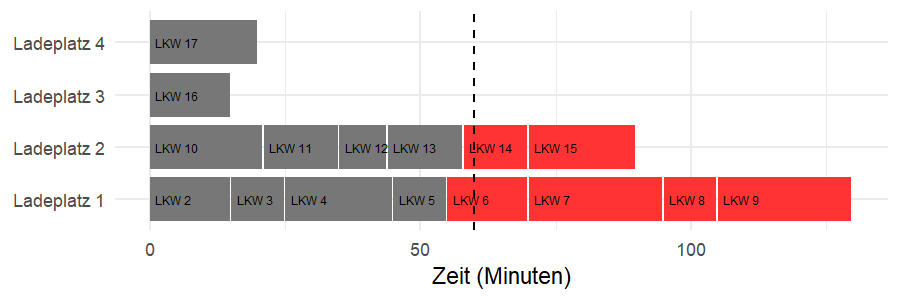
\includegraphics[width=\textwidth]{images/timelines/timelineTspCutExample1.png}
    \caption{Beispiel für einen per mTSP sortierten Zeitplan}
    \label{fig:tspCutExample1}
\end{figure}

In Abbildung \ref{fig:tspCutExample2} ist der Zeitplan aus Abbildung \ref{fig:tspCutExample1} auf einen 60 Minuten Slot angepasst worden. Zuerst wurden LKW 14 und LKW 15 vom Ladeplatz 2 entfernt und auf Ladeplatz 4 verschoben, da dies die einzige Kette ist, die noch vollständig auf einen anderen Platz passt. Die Kette von LKW 6 bis LKW 9 wurde auf Ladeplatz 4 verschoben, hier ist allerdings zu erkennen, dass diese dort nicht komlett hinein passt und somit LKW 8 und LKW 9 in diesem Slot nicht bearbeitet werden können. Außerdem haben sich die Zeitfenster der LKW am Anfang und Ende der zusammenhängenden Ketten leicht verlängert, da sowohl die verschobenen Teile, als auch die zurückgebliebenen Teile etwas längere Zeit brauchen, da hier kein optimaler Wechsel der Ladehilfsmittel mehr gegeben ist.

\begin{figure}[H]
    \centering
    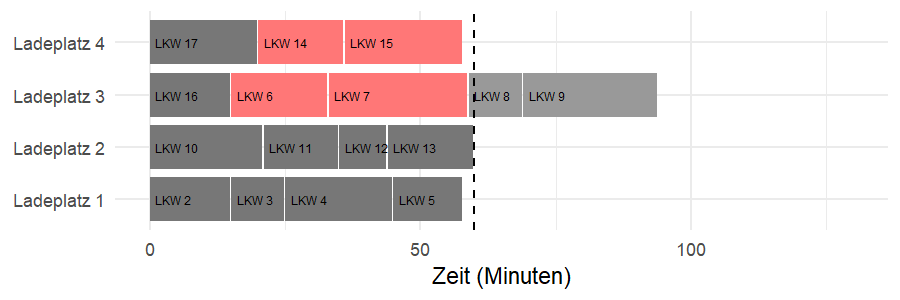
\includegraphics[width=\textwidth]{images/timelines/timelineTspCutExample2.png}
    \caption{Zeitplan aus Abb. \ref{fig:tspCutExample1} auf einen 60 Minuten Slot angepsst}
    \label{fig:tspCutExample2}
\end{figure}


\subsubsection{Vergleichswerte zur Auswertung generieren}

\todo{fcfs ausgangssituation generieren beschreiben}

Ein letzter Schritt, welcher nicht direkt für den zuvor beschriebenen Optimierungsalgorithmus benötigt wird, ist die Generierung eines Zeitplans zu Vergleichs- und Auswertungszwecken. Dieser Zeitplan soll die Reihenfolge der Abfertigung im unoptimierten Zustand nachbilden. Nötig ist dies, da kaum nutzbare, reale Testdaten vorhanden sind. Gerade um eine große Menge generierter LKW Buchungen auswerten zu können, macht es durchaus Sinn sich Gedanken zu machen, wie ein solcher Algorithmus arbeiteten könnte. Zusätzlich lassen sich hier auch noch einmal genaue Erkenntnisse und ein besseres Verständnis für die bisherige Ausgangssiuation gewinnen, wenn man sich klar macht, wie die LKW dort ankommen.

Prinzipiell kommen die LKW nach keinem wirklichen System an, wie bereits in Kapitel \ref{sec:analyse} herausgearbeitet wurde. Innerhalb des Slots kommen die LKWs theoretisch zu einer zufälligen Zeit. Somit wäre der Ansatz hier, die Liste der ankommenden LKW in eine zufällige Reihenfolge zu bringen und diese nach dem \glqq{}first come, first served\grqq{}-Prinzip zu sortieren. Für einen Ladeplatz ist da nicht viel Logik nötig, die Liste kann genau in dieser Reihenfolge übernommen werden. Für mehrere Ladeplätze müsste hier auch wieder die Zeitberechnung aus dem Optimierungsalgorithmus (siehe Kapitel TODO) herangezogen werden. Für die vorliegende Lösung wurde angenommen, dass die Abfertigungszeit, die jede Maschine braucht, sich nicht verändert. Ein Vorteil wird durch die beste Reihenfolge und die Einsparung von Fahrt- und Rüstzeiten erreicht. Das System zur Kostenberechnung selbst kann somit auch hier eingesetzt werden. Es müsste bei der Sortierung auf mehrere Plätze also nach jedem einsortierten LKW die entsprechende Dauer bis zur Fertigstellung des bisher letzten LKW berechnet werden und anschließend immer zum Ladeplatz mit der kürzesten Dauer ein LKW einsortiert werden. So wird nachgebildet, dass immer der Ladeplatz welcher als nächstes frei wird, den nächsten LKW aufnimmt.

Insgesamt lässt sich so eben auch genau das Ausgangsproblem nachbilden: Die LKW kommen wie sie wollen, es wird keine Rücksicht darauf genommen, welche Ressourcen benötigt werden. Somit kann es zufällig einmal passen, dass die richtige Maschine bereits Vorort ist, in der Regel wird dies aber nicht der Fall sein und somit ein hoher Wechselaufwand entstehen.
 % aktuell 21 Seiten



\newpage
\section{Prototypische Realisierung}
\label{sec:realisierung}
Nach der zuvor erstellen Konzeption folgt nun die Implementierung dieser Planungen. Beide Optimierungsansätze werden dabei weiterhin getrennt voneinander umgesetzt.

\subsection{Entwicklungsumgebung und Projektaufbau}

Beide Projekte sind als normale Java Projekte, ohne besonders Framework aufgebaut. Sie nutzen die zum Zeitpunkt der Entwicklung aktuellste Version 22 von OpenJDK. Zur einfacheren Verwaltung der genutzten Libraries wird das Build-Werkzeug Maven eingesetzt. Genutzt werden in den Projekten jeweils zwei Libraries. Zum einen Lombok (in der Version 1.18.30), welche automatische Codegenerierung über Annotations ermöglicht und einfach dazu dienen soll, den Fokus auf den für dieses Projekt wesentlichen Code zu legen, indem die Generierung von Gettern, Settern und Konstruktoren ausgelagert wird. Für den Test der Algorithmen wird JUnit verwendet (Version 5.8.1). Dessen Zweck ist es, übersichtliche und strukturierte Testfälle für die Algorithmen aufzubauen. Da es keine Benutzeroberfläche und neben den Algorithmen auch kaum weiterreichende Kontrollstrukturen gibt, ist dies die beste Möglichkeit, die Algorithmen lauffähig zu machen.



\subsection{Umsetzung Algorithmus 1 (RS)}

Die hier niedergeschriebenen Kapitel sollen dazu dienen, die konkreten Gedanken und Details der durchgeführten Implementierung zu beschreiben. Dabei wird vor allem auf die Struktur, aber auch wichtige Daten und Abläufe eingegangen. Sehr spezifische Details zu exakten Implementierung und Funktionsweise des Codes werden hier eher nicht beschrieben, dies wurde an wichtigen und komplexen Stellen durch Kommentare im Code übernommen. Für das allgemeine Verständnis der Implementierung ist dies aber auch nicht entscheidend und eine rein textuelle Beschreibung von komplexen Codestellen würde das Verständnis auch nicht unbedingt fördern.

\subsubsection{Aufbau und Entwurfsmuster}

\todo{Quelle MVC?!}

Implementiert wurde dieses Projekt nach dem Model-View-Controller (MVC) Muster. Gewählt wurde dieses zum einen, da es sich um ein einfaches und bekanntes Muster handelt. Da es sich hier hauptsächlich um die prototypische Implementierung der Algorithmen handelt und nicht um ein umfassendes Softwareprojekt, ist das Entwurfsmuster in diesem Fall auch nicht so entscheidend. Das MVC hat den Vorteil, dass es Datenstrukturen, Kontrollstrukturen und die Präsentation der Daten trennt. So kann die Darstellung der Daten übersichtlich getrennt werden, was eine spätere Implementierung dieser Algorithmen in einen anderen Softwarekontext erleichtert, weil so schon klare Datenschnittstellen definiert sind. Die Kontrollstrukturen sind in diesem Fall die Algorithmen, welche ebenfalls getrennt und übersichtlich abgelegt werden. Eine richtige View, also Benutzeroberfläche gibt es in diesem Fall noch gar nicht. MVC wird aber häufig auch wegen seiner guten Austauschbarkeit der Präsentation der Daten eingesetzt. Somit ist es hier später auch einfacher möglich, eine richtige Benutzeroberfläche anzusetzen.

Die Implementierung gliedert sich in bedeutende und zusammenhängende Bestandteile, welche im Folgenden einzeln genauer erläutert werden.


\subsubsection{TruckAdvices}

\begin{figure}[H]
    \centering
    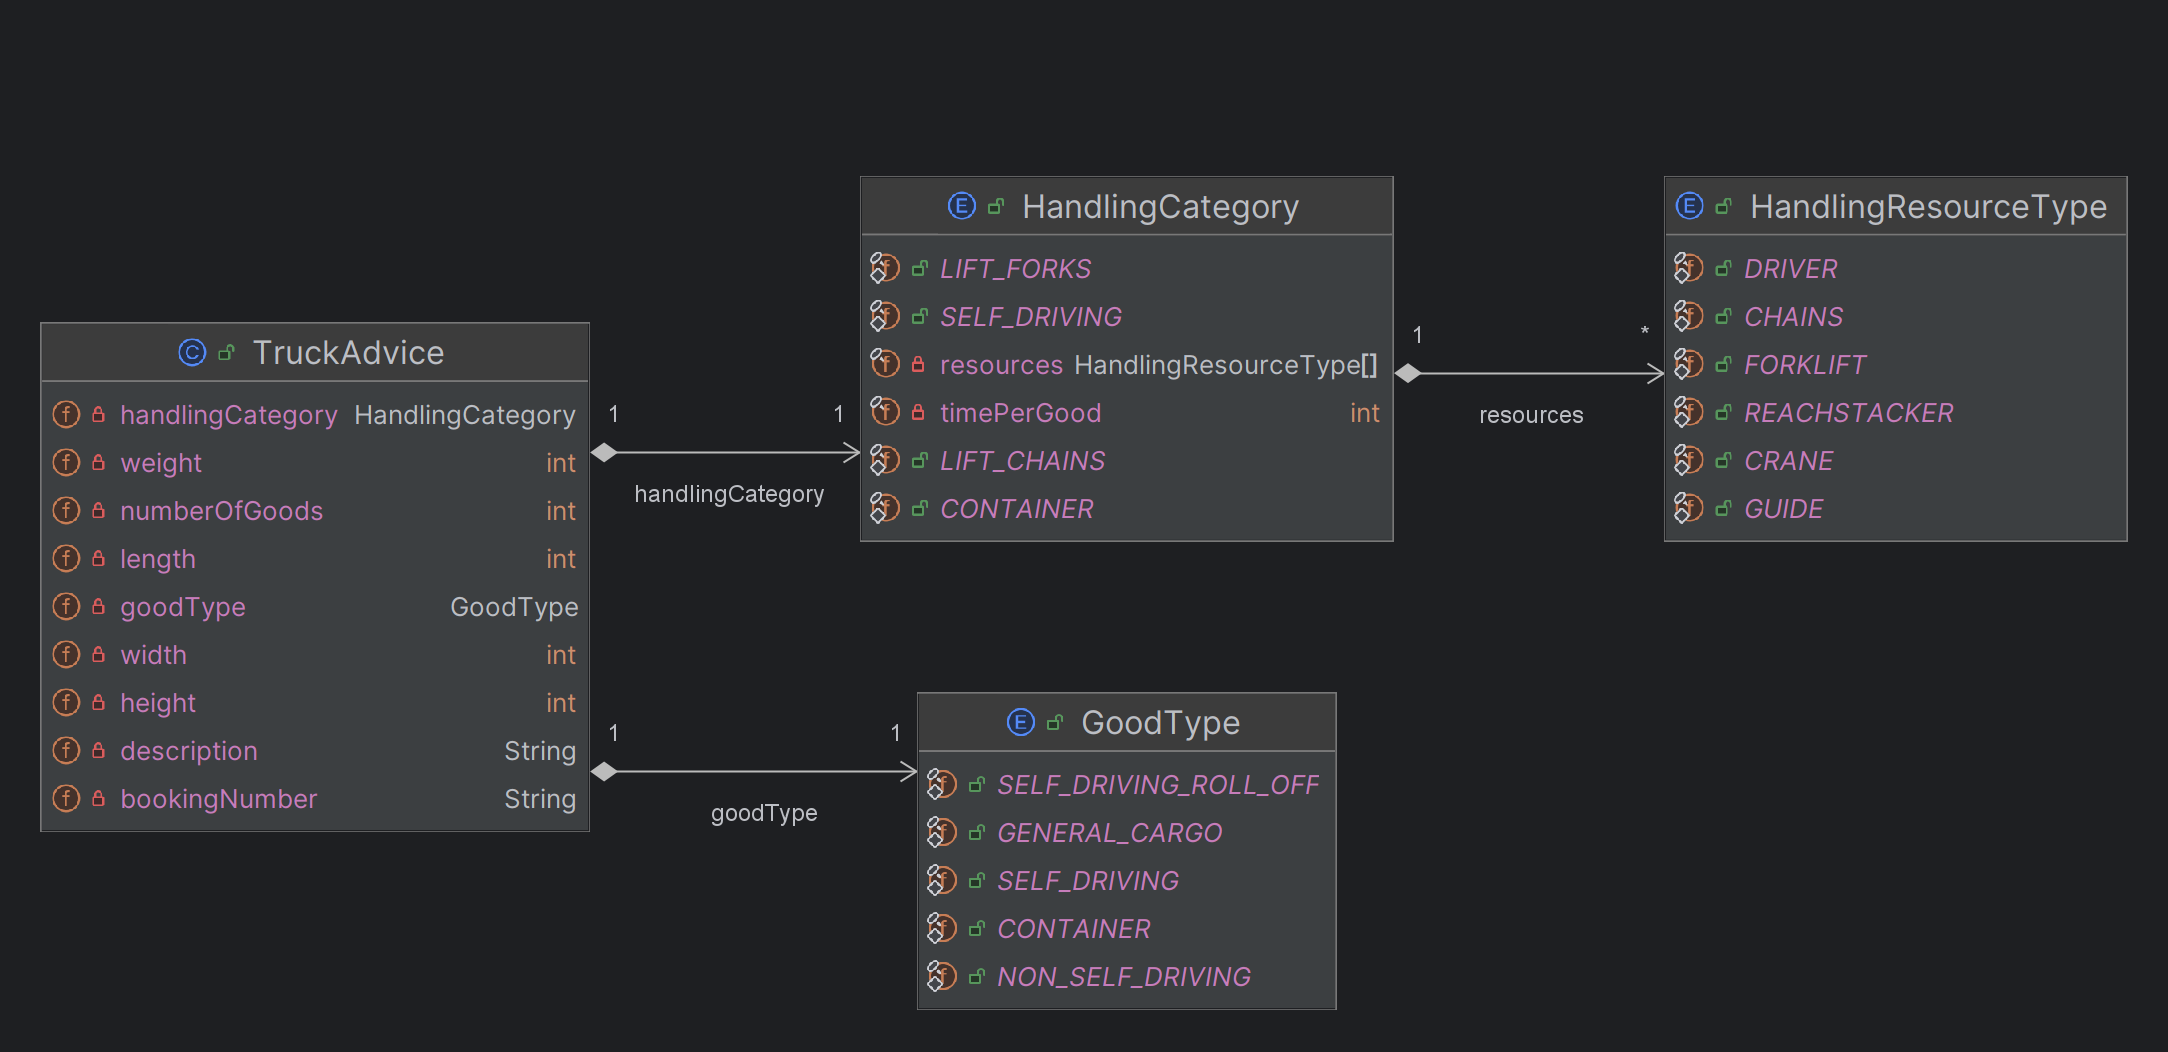
\includegraphics[width=\textwidth]{images/classDiagrams/TruckAdvice_ClassDiagram.png}
    \caption{Klassendiagramm der Modelklassen im Zusammenhang mit TruckAdvice}
    \label{fig:classDiagramTruckAdvice}
\end{figure}



Die Basis des Projekts bilden, wie bereits ausführlich herausgearbeitet wurde, die LKW Avisierungen am Terminal. Um die entsprechenden Daten zu halten, wurde eine passende Datenstruktur aufgebaut. Das Hauptobjekt ist dabei TruckAdvice, welches die eigentliche Avisierung eines LKW enthält. Dies sind alle Daten, die von einer entsprechend vorgeschalteten Benutzeroberfläche erfasst werden müssen, um eine sinnvolle Verarbeitung und Planung der Aufträge durchführen zu können. Darunter sind einige Parameter, welche für den hier entwickelten Algorithmus unumgänglich sind. Dies sind numberOfGoods und die HandlingCategory. Alle weiteren Daten, wie Warentyp, Beschreibung, Buchungsnummer, Gewicht und Ausmaße sind für diese Implementierung nicht von besonderer Wichtigkeit, dennoch sind sie wichtige Angaben die im späteren Ladeprozess im Hafen vollständig und korrekt sein sollten, um eine gute Vorbereitung zu gewährleisten und Fehler zu vermeiden. Aus Gründen der Datenhaltung und der leichteren Verarbeitung wurde entschieden, die ausgewählte Zeit bzw. den Slot nicht direkt im Objekt zu speichern, sondern über entsprechende Liste pro Slot, denen jeweils die TruckAdvice Objekte hinzugefügt werden.

Um eine Kategorisierung und eindeutige Bestimmung der gelieferten Güter zu ermöglichen, ohne Spielraum und Unklarheiten durch Freitextfelder zu erzeugen, wurden die wichtigsten Daten durch Enums erfasst. Diese erlauben auch eine spätere Anpassung oder Erweiterung der bisher vorgegebenen Daten. Bedeutender für die Planungsalgorithmen ist aber die HandlingCategory. Dies ist ein fester Satz von Arten, wie ein Gut abgeladen werden kann. Pro Kategorie kann hier eingestellt werden, wie lange es dauert, ein Gut dieses Typs vom LKW abzuladen. Außerdem kann eine Liste von Ressourcentypen (HandlingResourceType) angegeben werden, die zur Verarbeitung im Hafen nötig sind. Diese HandlingResourceTypes bilden die letzte Enum.

Alle Enums wurden mit Werten entsprechend der Analyse aus Kapitel \ref{sec:analyseAbfertigung} gefüllt. Folgende Werte sind dabei aktuell gesetzt, wobei Erweiterungen durch die Wahl des Typs Enum möglich sind, ohne umfangreichere Anpassungen vornehmen zu müssen: \todo{Enumwerte final?}

GoodType: CONTAINER, GENERAL\_CARGO, SELF\_DRIVING, SELF\_DRIVING\_ROLL\_OFF, NON\_SELF\_DRIVING

HandlingResourceTypes: FORKLIFT, CRANE, REACHSTACKER, GUIDE, DRIVER, CHAINS

HandlingCategory: 
\begin{itemize}
    \item LIFT\_CHAINS (timePerGood: 12, HandlingResourceTypes: CRANE, GUIDE, CHAINS)
    \item LIFT\_FORKS (timePerGood: 5, HandlingResourceTypes: DRIVER, GUIDE)
    \item SELF\_DRIVING (timePerGood: 8, HandlingResourceTypes: REACHSTACKER, CHAINS)
    \item CONTAINER
\end{itemize}



\subsubsection{Zeitplan}

\begin{figure}[H]
    \centering
    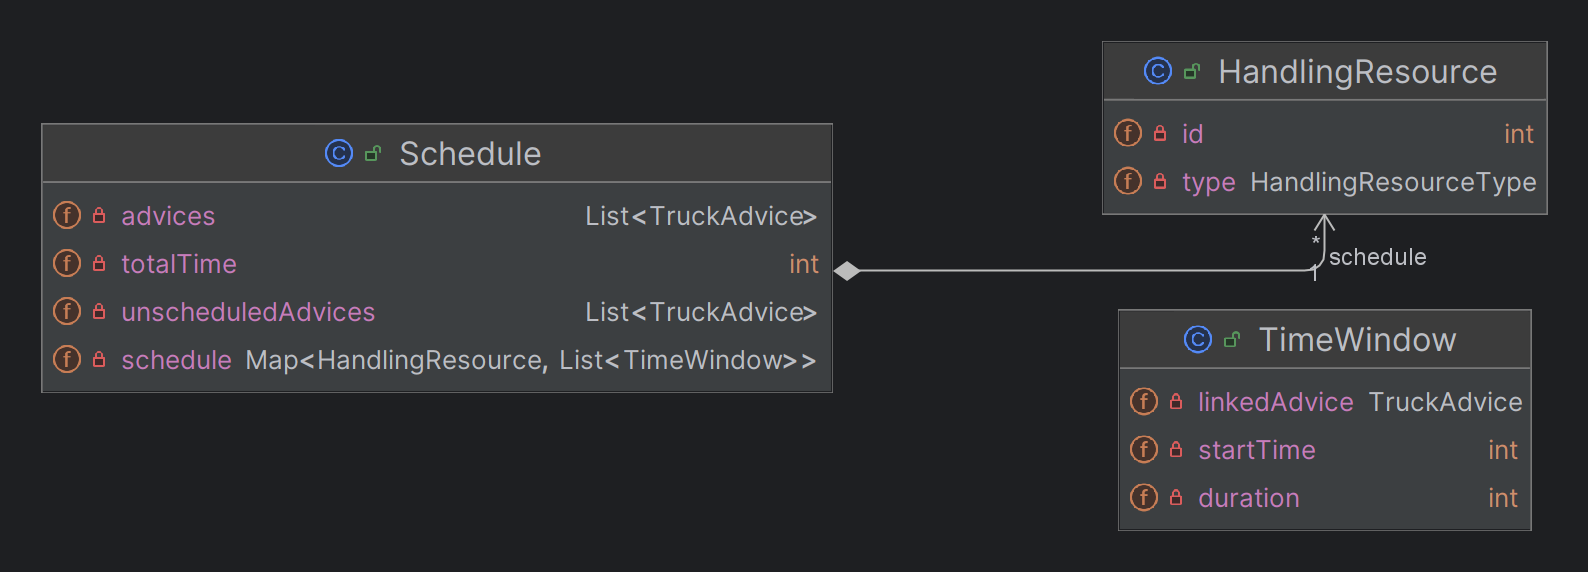
\includegraphics[width=\textwidth]{images/classDiagrams/Schedule_ClassDiagram.png}
    \caption{Klassendiagramm der Modelklassen im Zusammenhang mit Schedule}
    \label{fig:classDiagramSchedule}
\end{figure}

Ein wesentlicher Bestandteil des hier gezeigten Ansatzes ist die Erstellung eines Zeitplans (Schedule). Um also Algorithmen zu entwickeln, welche einen Zeitplan erzeugen können, musste zunächst einmal eine passende Datenstruktur mit entsprechenden Kontrollstrukturen entwickelt werden. 

Grundidee ist, dass ein Zeitplan aus verschiedenen parallelen Zeitachsen für unterschiedliche Ressourcen besteht. Der gesamte Zeitplan hat dabei eine eindeutige Gesamtlänge in Minuten, um die Länge eines Zeitslots darzustellen. Es ist dabei so, dass jede Zeitachse durch Zeitfenster (TimeWindow) belegt werden kann. Diese können nur nacheinander liegen und haben jeweils einen Startzeitpunkt und eine Dauer in Minuten. Die Datenstruktur eines Schedules ist deshalb relativ einfach aufgebaut: Eine Map beinhaltet jeweils die verfügbaren Ressourcen als Key und ordnet jeder Ressource eine Liste von TimeWindows zu, in denen diese bewegt ist. Die Liste der belegten Zeitfenster ist dabei immer nach Startzeit, also chronologisch sortiert. Um einen besseren Überblick über alle Avisierungen zu behalten und auch um alle noch nicht oder nicht mehr planbaren Avisierungen zu speichern, enthält ein Schedule Objekt jeweils eine Liste der entsprechenden TruckAdvices. 

Damit die Planungsalgorithmen mit einem Zeitplan arbeiten können, werden diverse, teils komplexere Abfragen und Operationen auf die Schedule Objekte benötigt. Um diese Operationen ohne Codedopplungen und separiert von dem Datenobjekt Schedule erreichbar zu machen, wurde dafür eine Klasse ScheduleTools angelegt. Alle Methoden sind dabei statisch, da sie auf einem übergebenen Schedule Objekt arbeiten und lediglich Abfragen darauf ausführen, ohne komplexere Daten halten zu müssen. Folgende Methoden sind verfügbar und können von allen Planungsalgorithmen genutzt werden:

\begin{itemize}
    \item \textit{findAvailableResourceByType(Schedule schedule, HandlingResourceType type, TimeWindow window): HandlingResource}

    Findet innerhalb des Zeitplans eine passende Ressource, die im angegebenen Zeitfenster verfügbar ist. Dies ist vor allem interessant, wenn nach der Suche von Zeitfenstern eine passende Ressource gebucht werden soll.    
    
    \item \textit {checkWindowsOverlapping(TimeWindow w1, TimeWindow w2): boolean}

    Prüft, ob zwei angegebene Zeitfenster zeitlich überlappen, d.h. ob sich diese zeitlich überschneiden oder ob sie einfach nacheinander gebucht werden können.
    
    \item \textit{findEmptyTimeWindows(Schedule schedule, HandlingResourceType resourceType): List<TimeWindow>}

    Diese Methode such alle verfügbaren Zeitfenster für einen bestimmten Ressourcen Typ innerhalb des Zeitplans. Dies ist vor allem interessant, um zu planen, wann freie Zeiträume für welche Avisierung verfügbar sind.
    
    \item \textit{getOverlappingWindows(Schedule schedule, List<TimeWindow> list1, List<TimeWindow> list2) List<TimeWindow>}

    Gibt eine Liste von Zeitfenstern zurück, in denen sich die Zeitfenster aus zwei separaten Listen überschneiden. Das ist vor allem interessant, um zu schauen, wann zwei oder mehr Ressourcen gleichzeitig verfügbar sind.
    
    \item \textit{cleanWindowList(List<TimeWindow> list): List<TimeWindow>}

    Entfernt alle Zeitfenster, die komplett in einem anderen enthalten sind. Es kann sonst möglicherweise zu Problemen kommen, wenn durch verschiedene Operationen keine saubere Liste erzeugt wurde, bei der alle Zeitfenster chronologisch und ohne Überschneidungen vorliegen.
    
    \item \textit{getBiggestWindow(List<TimeWindow> list): TimeWindow}

    Sucht das größtmögliche Zeitfenster aus einer übergebenen Liste heraus.
    
    \item \textit{getSmallestWindow(List<TimeWindow> list, int minTime): TimeWindow}

    Sucht das kleinstmögliche Zeitfenster aus einer übergebenen Liste heraus.
\end{itemize}

Viele der genannten Methoden sind durchaus komplex und bergen Fehlerpotenziale, insbesondere bei der Arbeit mit Zeitfenstern und deren Relationen zueinander. Innerhalb der eigentlichen Planungsalgorithmen werden allerdings viele der Methoden bereits intensiv eingesetzt, so konnten bereits viele Fehler durch manuelle Tests beseitigt werden. Zu einigen Methoden konnten auch automatisierte Testfälle zur Überprüfung geschrieben werden \todo{Automatisierte Tests schreiben?}. Aus Zeitgründen und einer Kosten-Nutzen-Abwägung wurde entschieden, dass dieser Aufwand und Umfang zur Fehlersuche ausreicht. Nach vielen manuellen Überprüfungen konnten schlussendlich keine Fehler mehr entdeckt werden, die Fehlerrate sollte also wenn überhaupt vorhanden, sehr gering sein.



\subsubsection{Planungsalgorithmen}

Die Implementierung der Algorithmen ist der zweite bedeutende Bestandteil bei der Entwicklung dieses Projekts. Wie in der Planung beschrieben, sollen mehrere Sortierungsverfahren parallel implementiert werden, um am Ende einen Vergleich anstellen zu können. Um eine möglichst gute Modularität, Austausch- und Erweiterbarkeit zu erzielen, bauen wurde jeder Algorithmus in einer eigenen Klasse umgesetzt, welche von der abstrakten Hauptklasse Scheduler erbt. Diese definiert eine feste Methode, welche einen Zeitplan für einen Zeitslot erzeugt, wenn sie eine Liste von gebuchten LKW, eine Liste der zu diesem Zeitpunkt im Terminal verfügbaren Ressourcen und die Länge des Zeitslots übergeben bekommt. Eingangs- und Ausgangsschnittstellen sind somit klar definiert und die Logik dazwischen kann beliebig ausgetauscht werden, auch zukünftig.

\begin{figure}[H]
    \centering
    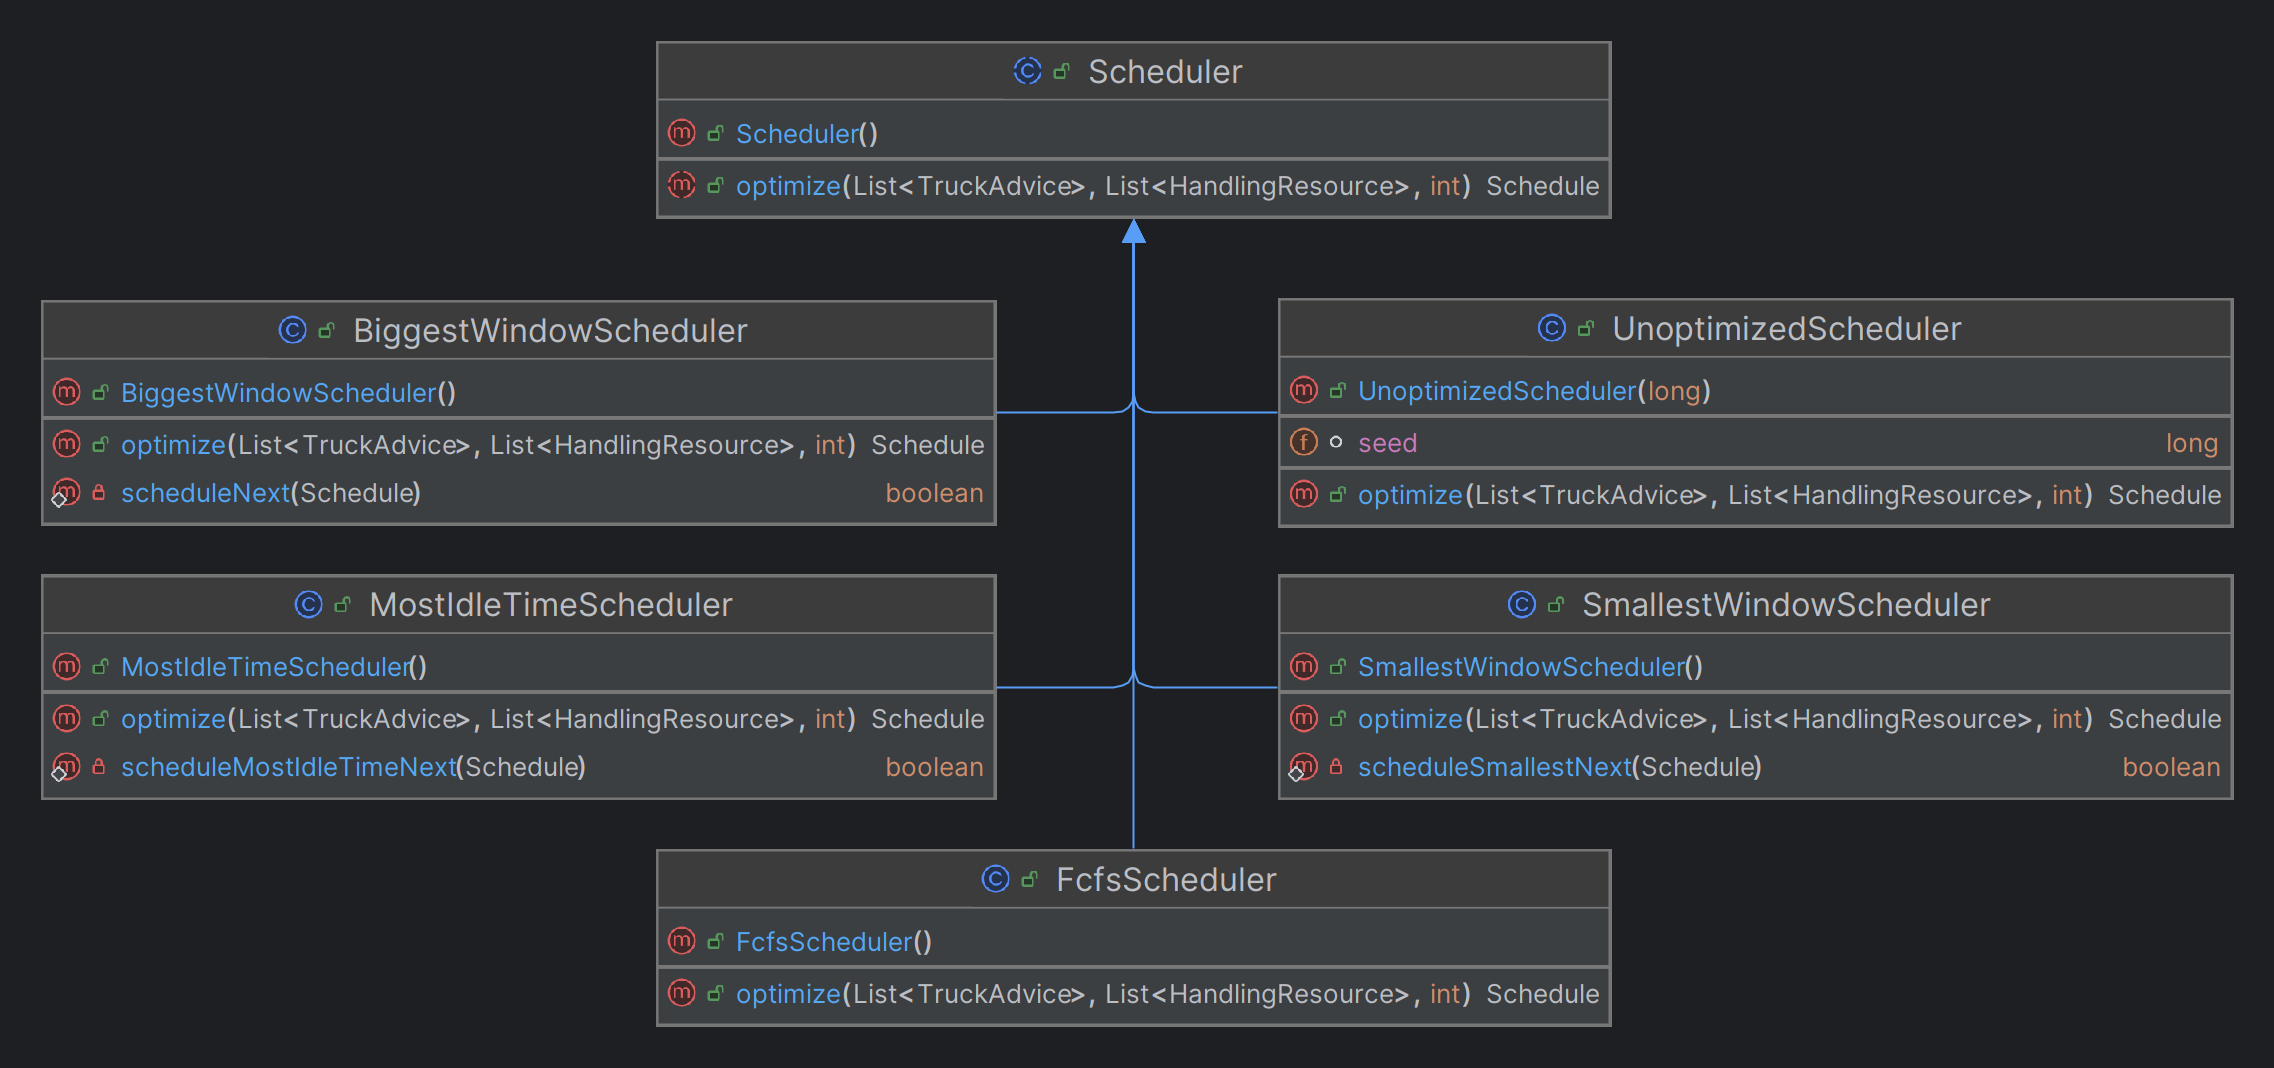
\includegraphics[width=\textwidth]{images/classDiagrams/Scheduler_ClassDiagram.png}
    \caption{Klassendiagramm aller Controllerklassen, die von Scheduler erben}
    \label{fig:classDiagramScheduler}
\end{figure}

Bei der Entwicklung der Algorithmen wurde darauf geachtet, soweit Zufallswerte eingesetzt wurden, diese mit der Möglichkeit auszustatten, Seeds zu übergeben. Dies soll die Wiederholbarkeit von späteren Testläufen sicherstellen. Im Praxiseinsatz kann hier einfach mit zufälligen Werten oder Standardseeds gearbeitet werden.
\todo{- Algorithmen erklären? Noch mehr schreiben?!}


\subsubsection{Analyse der Zeitplanungen}

\todo{Klassendiagramm?}

Alle nach den unterschiedlichen Verfahren erstellten Zeitpläne liegen nun in einem einheitlichen Format als Schedule-Objekt vor. Dies ermöglicht auch eine über alle Verfahren einheitliche Auswertung. Um im Verlauf dieser Arbeit Analysen und eine Evaluation durchführen zu können, wurde aus diesem Grund eine eigene Controller-Klasse ScheduleAnalyser erstellt, welche alle interessanten Werte aus dem Schedule berechnet und als einheitliches ScheduleAnalysis-Objekte speichert und zurück gibt. 

Folgende Werte werden dabei berechnet:

\todo[inline]{Alle Attribute von ScheduleAnalysis auflisten, Rechenweg und Zweck erklären, Bilder zur Verdeutlichung hinzufügen?}

\begin{itemize}
    \item \textit{scheduledJobs:} Die Anzahl der LKW, die erfolgreich in den Zeitslot eingeplant werden konnten. Die Erhöhung dieses Wertes ist da Hauptziel der Optimierung, eine insgesamt effizientere Planung sollte am Ende dafür sorgen, dass mehr LKW innerhalb des gleichbleibenden Slots bearbeitet werden können.
    \item \textit{unscheduledJobs:} Die Anzahl von LKW, die zeitlich nicht mehr in den Slot gepasst haben.
    \item \textit{totalJobs:} Die Gesamtanzahl der avisierten LKW, welche versucht wurden, auf den Slot zu verteilen (entspricht scheduledJobs+unscheduledJobs).
    \item \textit{totalTimeToComplete:} Die Dauer in der innerhalb des Slots Ressourcen belegt werden. Dies ist vor allem interessant, um ein Maß für die Optimierung zu haben, wenn der Slot nicht komplett mit LKW ausgefüllt ist. Je schneller dann die Arbeit beendet ist, desto mehr können die Ressourcen an anderer Stelle eingesetzt werden.
    \item \textit{averageWaitingTime:} Die durchschnittliche Zeit von Beginn des Slots, bis zum Beginn der Bearbeitung eines LKW. 
    \item \textit{maxTimeToWait:} Die maximale Zeit, welche ein LKW seit Beginn des Slots warten muss, bis er abgeladen wird.
    \item \textit{idleTotal:} Die Summe der Leerlaufzeiten aller Ressourcen, in denen sie für keinen Jobs eingebunden sind.
    \item \textit{idleToComplete:} Die Summe der Leerlaufzeiten aller Ressourcen, bis alle Aufträge abgearbeitet sind. Ein relatives Maß, falls zu wenig LKW für den ganzen Slot vorhanden sind. Die Gesamtleerlaufzeit würde hier sehr stark nach oben gehen, obwohl Ressourcen dann evtl. ganz woanders eingesetzt werden könnten.
    \item \textit{idleBetweenJobs:} Die Summe der Leerlaufzeiten aller Ressourcen zwischen Aufträgen. Vor Beginn des ersten LKW und nach Ende des letzten LKW kann eine Ressource möglicherweise an anderer Stelle eingesetzt werden. Viele auseinander gezogene Jobs mit vielen kurzen Leerlaufzeiten zwischendurch sind unschön für eine optimale Auslastung.
\end{itemize}


\subsubsection{JUnit Tests}

\todo{Generierungsklasse und CSV Exporter genauer erläutern?}

Um schlussendlich sinnvolle Testläufe und Auswertungen der implementierten Algorithmen durchführen zu können, wurde ein Basis für JUnit Test geschaffen. Zum einen braucht es hier die Möglichkeit passende und realitätsnahe Eingangsdatensätze, also insbesondere Listen von TruckAdvices zu generieren. Dafür wurde eine entsprechende Methode geschrieben, welche mit Zufallswerten arbeiten kann. Wie auch schon bei der Implementierung der Algorithmen erwähnt, ist es hier besonders wichtig, mit Seeds zu arbeiten, um wiederholbare Testläufe zu erzeugen, wenn diese Auf Zufallseingaben basieren. Aus diesem Grund enthält jeder Testfall zunächst ein Random-Objekt mit festgelegten Seed, aus dem in dieser Testmethode benötigten Werte generiert werden. Der zweite wesentliche Bestandteil jedes Tests, ist der eigens entwickelte CsvExporter. Diese Klasse ermöglicht es sehr einfach die Testreihen und Datensätze jedes Durchlaufs in entsprechende CSV-Dateien zu schreiben. Dies ist ein einfaches Format zur standardisierten und strukturierten Speicherung von Daten bzw. Datentabellen \todo{Quelle?}. So können die Daten zur weiteren Auswertung sehr leicht in R-Skripte importiert und weiterverarbeitet werden.



\subsection{Umsetzung Algorithmus 2 (TSP)}

Von der grundsätzlichen Struktur und den Gedanken zum Aufbau unterscheidet sich die Implementierung dieses Algorithmus gar nicht stark von der zuvor beschriebenen Implementierung des anderen Algorithmus. Aus diesem Grund hat auch die nachfolgende Struktur der Beschreibung eine große Ähnlichkeit. Der Fokus wird hier deshalb auch konkreter auf spezielle Entscheidungen und Unterschiede gelegt, gemeinsame Entscheidungen werden hier nicht so tief erläutert und begründet. Auch in diesem Fall wird mehr Fokus auf die Beschreibung der wichtigen Strukturen, Daten und ABläufe gelegt. Konkrete Beschreibungen von komplexen Codestellen, welche auch für das allgemeine Verständnis der Implementierung nicht so wichtig sind, werden auch hier eher durch Kommentare im Code übernommen.

\subsubsection{Aufbau und Entwurfsmuster}

Es wurde ebenfalls das Model-View-Controller Muster gewählt. Auch hier ist die Trennung von Daten- und Kontrollstrukturen sehr sinnvoll, da sich so die Datenobjekte und Schnittstellen gut von den eigentlichen Algorithmen trennen lassen. Auch wenn sie hier ebenfalls noch nicht implementiert wurde, lässt sich eine Benutzeroberfläche so später sehr einfach hinzufügen bzw. die Kontrollstrukturen in eine bestehende Oberfläche integrieren. 

Die Implementierung lässt sich in einige Hauptbestandteile gliedern, welche in den folgenden Kapiteln genauer beschrieben werden.

\subsubsection{TruckAdvices}

Die Modellstruktur der LKW Avisierungen ähnelt auch sehr der Umsetzung des anderen Algorithmus. Die grundsätzlich gespeicherten und verarbeiteten Daten sind dabei aus Endnutzer Sicht im Hauptobjet TruckAdvice identisch. Der Unterschied ist in diesem Fall hauptsächlich die Implementierung der HandlingCategory. Einer Kategorie ist dabei jeweils die benötigte Maschine (HandlingMachine) zum Abladen zugewiesen. Eine HandlingMachine ist wiederum charakterisiert durch die mit ihrer Nutzung verbundenen Zeitaufwände, also Aufbauzeit (setupTime), Ladezeit pro Gut (timePerGood) und Abbauzeit (endTime). Im Vergleich zu dem anderen Ansatz findet hier eine deutlich größere Abstraktion statt. Während im anderen Fall konkrete Ressourcen bekannt sind, steht in dieser Umsetzung jede Ressource stellvertretend für alle in diesem Zusammenhang benötigten weiteren Ressource, wie entsprechende Fahrer oder Einweiser etc. Hier wird der Fokus dafür mehr auf die Berechnung des Zeitaufwands gelegt, was in der anderen Implementierung nicht der Fall war. 

\begin{figure}[H]
    \centering
    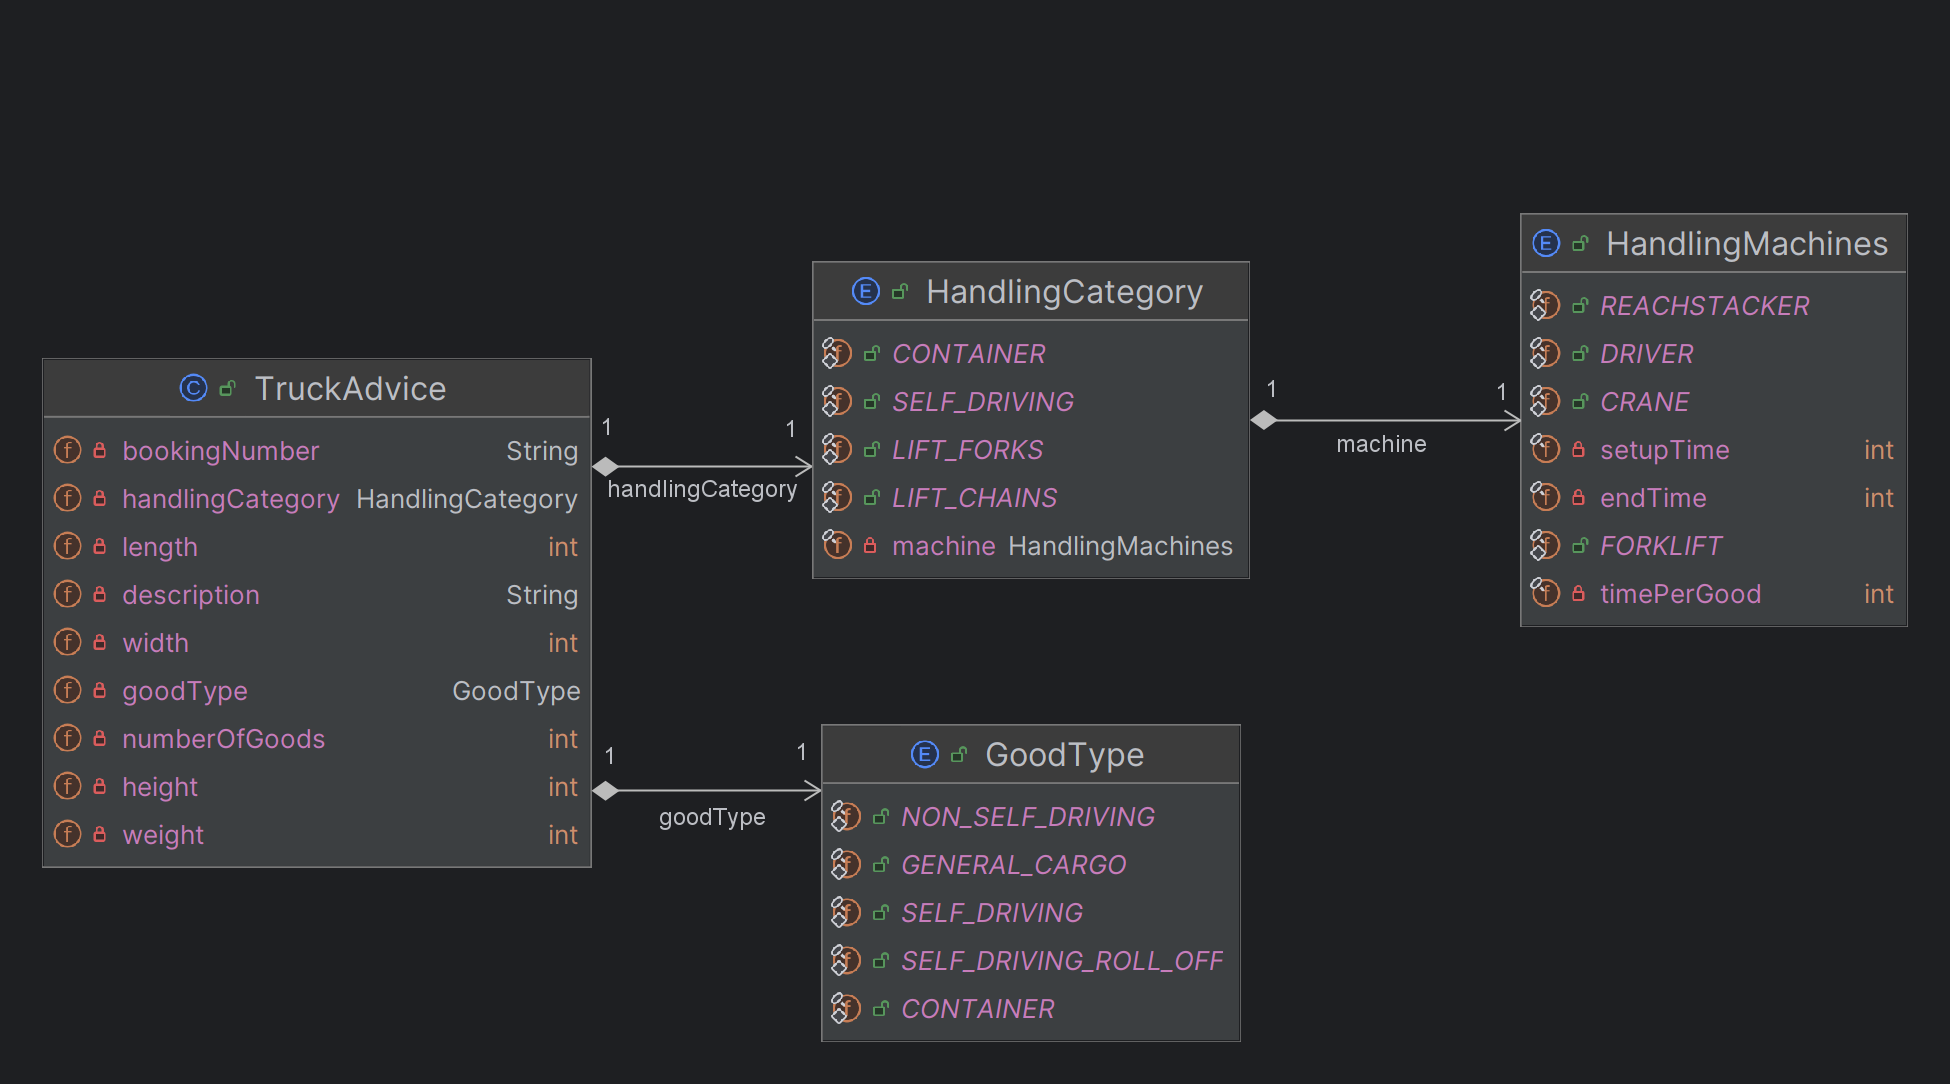
\includegraphics[width=\textwidth]{images/classDiagrams/TSP_TruckAdvice_ClassDiagram.png}
    \caption{Klassendiagramm der Modelklassen im Zusammenhang mit TruckAdvice}
    \label{fig:tspClassDiagramTruckAvice}
\end{figure}


Auch hier wurden alle Enums mit Werten entsprechend der Analyse aus Kapitel \ref{sec:analyseAbfertigung} gefüllt. Folgende Werte sind dabei aktuell gesetzt, wobei Erweiterungen durch die Wahl des Typs Enum möglich sind, ohne umfangreichere Anpassungen vornehmen zu müssen: \todo{Enum Werte final?}

GoodType: CONTAINER, GENERAL\_CARGO, SELF\_DRIVING, SELF\_DRIVING\_ROLL\_OFF, NON\_SELF\_DRIVING

HandlingCategory:
\begin{itemize}
    \item LIFT\_CHAINS (HandlingMachine: CRANE)
    \item LIFT\_FORKS (HandlingMachine: FORKLIFT)
    \item SELF\_DRIVING (HandlingMachine: DRIVER)
    \item CONTAINER (HandlingMachine: REACHSTACKER)
\end{itemize}

HandlingMachines:
\begin{itemize}
    \item CRANE(timePerGood: 10, setupTime: 30, endTime: 10)
    \item FORKLIFT(timePerGood: 5, setupTime: 15, endTime: 5)
    \item REACHSTACKER(timePerGood: 3, setupTime: 15, endTime: 10)
    \item DRIVER(timePerGood: 10, setupTime: 5, endTime: 2)
\end{itemize}



\subsubsection{TSP Graph}

Die Besonderheit dieses Algorithmus ist, dass es hier keine bloße Liste von Avisierungen gibt, welche entsprechend geplant werden soll. Es musste in diesem Fall eine Datenstruktur geschaffen werden, welche einen Graphen darstellen kann. Die implementierten Lösungsverfahren sollen dann das so aufbereitete TSP übergeben bekommen und einen optimierten Zeitplan erstellen.

Um diesen Graphen darzustellen, wurde die abstrakte Model-Klasse \textit{GraphNode} erstellt. Sie dient als Superklasse für alle Knotentypen in diesem Graphen. Ein Knotentyp ist, wie bereits angerissen, das TruckAdvice, also die schlussendlichen Aufgaben, welche geplant werden sollen. Zusätzlich wurde die GraphNode \textit{Loader} eingeführt. Sie wird für die Berechnung eines mTSP, also einer Optimierungsaufgabe mit mehreren Ladeplätzen benötigt und ist Teil der Implementierung des in der Planung genannten Verfahrens zur Transformation von mTSP in normale TSP (siehe Kapitel \ref{sec:mstpTransofrmation}). Entscheidende Werte des Graphen sind nun die Kosten an den Kanten zwischen den Knoten. Da es sich hier um einen vollständigen, gerichteten Graphen handelt und die Kostenberechnung in dieser Umsetzung dynamisch anhand von Start- und Zielknoten der Kante erfolgt, besitzt jede GraphNode eine Methode zur Kostenberechnung zu einem beliebigen anderen Knoten, welcher dieser Methode übergeben werden kann. So kann der Graph dynamisch gehalten werden, ohne vorab Berechnungen anstellen zu müssen und der Graph selbst kann sehr einfach in einer Liste von GraphNode-Objekten gespeichert werden.

\begin{figure}[H]
    \centering
    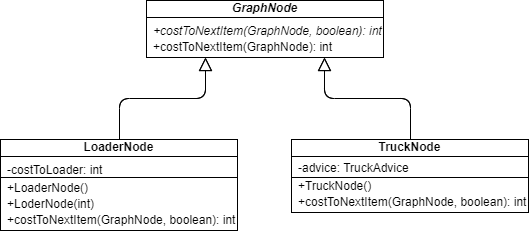
\includegraphics[width=0.7\textwidth]{images/classDiagrams/TSP_Graph_ClassDiagram.png}
    \caption{Klassendiagramm der Modelklassen im Zusammenhang mit dem Graphen}
    \label{fig:tspClassDiagramGraph}
\end{figure}


\subsubsection{Zeitplan}

Der Zeitplan selbst, also die Datenstruktur, welche schlussendlich von den TSP Lösungsverfahren erzeugt wird, ist hier einfacher aufgebaut. Sie bietet aber auch hier den großen Vorteil, dass auch ein über die Algorithmen einheitliches Ausgabeformat erzeugt wird. Ein Zeitplan enthält dabei grundsätzlich zwei Listen: Eine Liste (loaderAdvices), welche wiederum eine Liste von TruckAdvices enthält. Die erste Liste spiegelt dabei die unterschiedlichen Ladeplätze wieder, denen jeweils über die innere Liste eine Menge von Avisierungen zugeordnet ist. Die innere Liste ist dabei nach Reihenfolge der Abfertigung sortiert. Eine zweite, einfache Liste von TruckAdvices (unscheduled), speichert alle LKW, welche nicht (mehr) in den Zeitplan gepasst haben.

\begin{figure}[H]
    \centering
    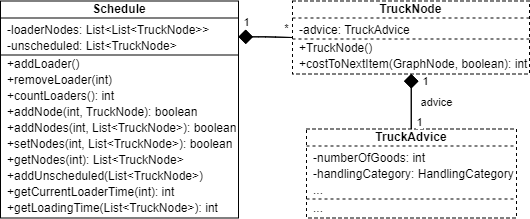
\includegraphics[width=\textwidth]{images/classDiagrams/TSP_Schedule_ClassDiagram.png}
    \caption{Klassendiagramm der Modelklassen des Zeitplans}
    \label{fig:tspClassDiagramSchedule}
\end{figure}


\subsubsection{Implementierung von TSP Lösungsverfahren}

Die Implementierung von Lösungsverfahren für das TSP ist der zentrale Teil des Projekts und für die eigentliche Optimierung zuständig. Um eine leichte Austauschbarkeit des Algorithmus zu erzielen, wurde auch hier eine erweiterbare Implementierung entwickelt, welche die abstrakte Klasse \textit{TspAlgorithm} nutzt (siehe Klassendiagramm in Abb. \ref{}\todo{ref}). Alle konkreten Implementierungen erben von dieser und können so über eine einheitliche Schnittstelle aufgerufen werden, welche aus einer Liste von TruckAdvices und der Anzahl von Ladeplätzen eine bestmögliche Verteilung, einen Schedule erzeugt.

\begin{figure}[H]
    \centering
    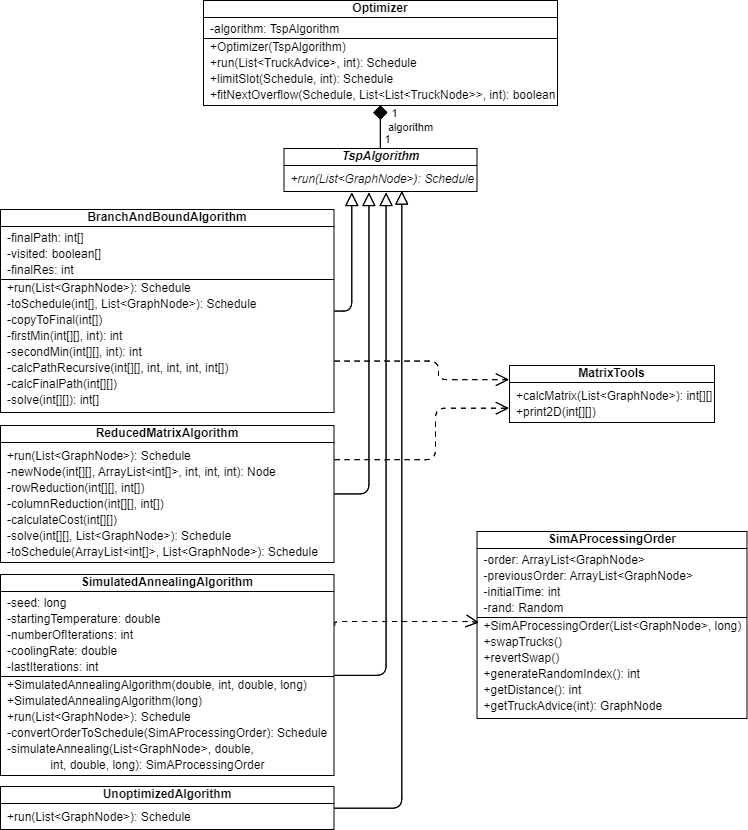
\includegraphics[width=\textwidth]{images/classDiagrams/TSP_Optimizer_ClassDiagram.png}
    \caption{Klassendiagramm der Controllerklassen zur Lösung des TSP}
    \label{fig:tspClassDiagramOptimizer}
\end{figure}

Die Implementierung von passenden Verfahren erweist sich bei genauerer Betrachtung als nicht trivial. Insbesondere, da neben der reinen Implementierung auch eine korrekte Funktionsweise getestet und sichergestellt werden müsste. Die folgenden Umsetzungen orientieren sich deshalb an den Java-Implementierungen der Computer Science Education-Plattform GeeksForGeeks \cite{geeksForGeeks}. Die Qualität und Funkionsfähigkeit der Codes wurde dabei durch Tests bei der Implementierung, Prüfungen gegeneinander und auch durch Prüfung der Abläufe mit Hilfe von anderen Quellen (siehe das Kapitel \ref{sec:tspVerfahrenPlanung} zur Planung der Verfahren) sichergestellt.

Bei der Implementierung der Verfahren sind einige Besonderheiten und Auffälligkeiten sichtbar geworden, auf welche hier einmal detailliert eingegangen werden soll:

\textbf{Simulated Annealing:} Dieser Algorithmus ist von der Implementierung und von der Nachvollziehbarkeit her das einfachste und verständlichste Verfahren. Auf die genaue Funktionsweise wurde bereits in der Konzeption eingegangen. Die Eingangsparameter sind hier sehr einfach, gearbeitet wird hier zunächst einmal direkt mit der Graph-Datenstruktur, wie sie zuvor beschrieben wurde. Um die Reihenfolge und die Tauschoperationen leichter abbilden zu können, wurde die Klasse \textit{SaProcessingOrder} eingeführt. Hier wird Simulated Annealing mit dem zufälligen Tausch von zwei Knoten des Graphen durchgeführt. Die Klasse erlaubt es diese Tauschoperationen auf einer temporären Kopie des Eingangsgraphen durchzuführen und kann gleichzeitig auch den letzten Tausch rückgängig machen, falls dies gewünscht ist. Ein besonderer Schritt dieses Verfahrens ist es, dass über Schleifen ein Abkühlungsprozess nachgebildet wird. Dieser Prozess folgt einigen Parametern, hauptsächlich Starttemperatur, Abkühlungsrate und Anzahl von Iterationen. Das Festlegen dieser Parameter ist eine Herausforderung und hängt von vielen Faktoren, unter anderem auch der Art der Eingangswerte des Algorithmus ab. Aus diesem Grund wurde die Bestimmung und Bewertung der besten Werte in den Evaluationsteil dieser Arbeit ausgelagert, dort werden dann alle Tests mit Realdaten gebündelt durchgeführt. Abschließend muss das interne SaProcessingOrder-Objekt noch in ein allgemeingültiges Schedule-Objekt umgewandelt werden. Da dies ein teils spezifischer Vorgang ist, der sich von dem der anderen Algorithmen unterscheiden, wurde dies auch noch als direkter Teil der Simulated Annealing Algorithmus Klasse implementiert. Bei der Ausführung der Klasse fiel schon bei der Implementierung auf, dass es gewisse Grenzen gibt, wenn der Eingangsgraph größer wird. Dies betrifft hier gar nicht so sehr die Ausführungsdauer, viel mehr kommt die Größe des Arbeitsspeichers an seine Grenzen. Eine genauere Betrachtung mit praxisbezogenen Daten soll auch hier in der Evaluation stattfinden.

\textbf{Branch and Bound:} Die Besonderheit dieser Implementierung ist, dass sie auf Basis einer Kostenmatrix arbeitet. Um den Implementierungsaufwand geringer zu halten und um die fertige Implementierung von GeeksForGeeks \cite{geeksForGeeksBnB} in Teilen Nutzen zu können, wurde zunächst eine Methode entwickelt, welche die Graph-Datenstruktur in eine Matrix aus Integer-Werten überführen kann. Da die Berechnungsschritte bereits alle implementiert waren, ist dies aber sehr einfach möglich, indem über Schleifen einmal jede Kombination vorgerechnet und in einem zweidimensionalen Array gespeichert wird. Da diese Matrix auch im Reduced Matrix Verfahren gebraucht wird, wurde die entsprechende Methode in die eigene Klasse \textit{MatrixTools} ausgelagert. Da das eigentliche Finden des kürzesten Weges wie erwähnt nicht ganz trivial ist, wurden alle nun folgenden Lösungsmethoden weitgehend aus dem Implementierungsbeispiel übernommen. Schlussendlich muss nun nur noch eine Methode zur Überführung in das bekannte Schedule-Objekt erfolgen. Auch bei diesem Verfahren fielen schnell Grenzen auf, diese sind sogar wesentlich früher erreicht, als bei Simulated Annealing. Hier ist allerdings die Ausführungszeit der limitierende Faktor. Es werden schnell extrem hohe Rechenzeiten erreicht, welche mit dem Hinzufügen einzelner Knoten exponentiell ansteigen, sodass schon mit sehr wenigen Knoten Ausführungszeiten erreicht werden, welche auch über einige Stunden und somit den sinnvoll nutzbaren Rahmen hinaus gehen. Auch hier folgt eine genauere Auswertung im Evaluationsteil dieser Arbeit.

\textbf{Reduced Matrix:} Das dritte Lösungsverfahren nutzt, wie der Name Reduced Matrix Verfahren auch schon vermuten lässt, ebenfalls eine Kostenmatrix als Eingangsformat. Die entsprechende Berechnungsmethode wurde schon für das Branch and Bound Verfahren entwickelt und kann hier wieder genutzt werden. Die danach benötigten Methoden zur Reduzierung und Berechnung des kürzesten Pfades wurden ebenfalls weitgehend aus dem Beispiel von GeeksForGeeks \cite{geeksForGeeksRm} übernommen. Auch hier wäre eine komplette Eigenentwicklung sehr komplex und fehlerträchtig. Auch in diesem Fall folgt am Ende noch eine Überführung der speziellen internen Lösung des Algorithmus in ein allgemeines Schedule-Objekt. Bei der Ausführung hat sich auch in diesem Verfahren schnell gezeigt, dass die mögliche Größe der lösbaren Graphen sehr begrenzt ist. Hier liegt es erneut an der Größe des verfügbaren Arbeitsspeichers, der vermutlich durch eine große Zahl von gespeicherten Matrizen sehr schnell ausgenutzt wird. Eine genauere Evaluation der Grenzen folgt auch hier zusammen mit der Auswertung der anderen Verfahren.

\textbf{Unoptimized:} Dies ist kein Lösungsverfahren für das TSP, in dieser Klasse wurde die geplante Generierung von Vergleichswerten umgesetzt. Sie erzeugt aus den Buchungen einen Zeitplan, wie er theoretisch vor einer Optimierung aussehen würde. Da es sich anbietet, hier das gleiche Ein- und Ausgabeformat zu verwenden, wie aus auch die TSP Algorithmen tun, wurde auch diese Klasse als Subklasse von TspAlgorithm implementiert. So sind die Werte im optimierten und unoptimierten Zustand direkt und sehr einfach vergleichbar.

Insgesamt ist zu den Algorithmen und deren Implementierung anzumerken, dass deren Hauptzweck ist, einen Eindruck davon zu bekommen, dass der Optimierungsansatz über das TSP valide ist und zu guten Lösungen führt. Es sollten hier auch Verfahren auf deren Vor- und Nachteilen, sowie auf deren Verwendbarkeit für das hier vorliegende Szenario untersucht werden. Es hat sich aber auch gezeigt, dass eine Umsetzung durchaus sehr komplex und nicht trivial ist. Insbesondere gute und optimierte Verfahren, welche schnell die beste Lösung liefern, sind nicht einfach umzusetzen und deshalb auch ein Problem, mit welchem sich die Informatik schon sein Jahrzehnten beschäftigt \cite{travelingSalesman}. Aus diesem Grund ist es auf jeden Fall ein Erfolg, dass hier zielführende Lösungen gefunden wurden, dennoch kann hier sicherlich mit deutlich mehr Aufwand ein besseres Verfahren gefunden werden. Durch die modulare Implementation sollte dies aber auch gut ersetzbar sein.

\subsubsection{Optimizer}

Um eine einfachere Austauschbarkeit der TSP Verfahren zu erzielen, wurde die Optimizer Klasse eingeführt. Sie ermöglicht es, dynamisch eine der zuvor entwickelten Algorithmusklassen zu verwendet. Gleichzeitig können aber über alle Verfahren einheitliche Arbeitsschitte an einer Stelle durchgeführt werden, ohne dass es einer mehrfachen Implementierung bedarf. Zunächst gehört dazu einmal das Auffüllen der Graphen mit den Dummy Ladeplatz Knoten (Loader-Objekte). Die werden in allen TSP Verfahren benötigt, wenn ein mTSP Problem mit mehreren Plätzen vorliegt und kann somit ausgelagert werden. Der Optimizer ermöglicht es aber gleichzeitig, eine von außen abstrahierte und vereinfachte Darstellung zu nutzen. Hier wird lediglich eine Liste von TruckAdvices, also den Eingaben der LKW Fahrer benötigt und die Anzahl der verfügbaren Ladeplätze. Die interne Erstellung des Graphen erfolgt dann erst gekapselt in der Optimizer Klasse. Der zweite ausgelagerte, da gemeinsame Aspekt, ist das Zuschneiden der optimierten Reihenfolgen auf einen begrenzten Slot. Nachdem die beste Abfertigungsreihenfolge durch die Verfahren gefunden wurde, ist die Überführung in einen Zeitplan prinzipiell nicht kompliziert. Für einen Ladeplatz ist die Reihenfolge bereits fertig und muss nur noch entsprechend zum Schedule-Objekt hinzugefügt werden. Für mehrere Ladeplätze müssen die TruckAdvices zwischen den Loader-Knoten jeweils in eine eigene Teilliste im Schedule gespeichert werden. Etwas aufwändiger dagagen ist die Implementierung der in Kapitel \ref{sec:tspToSchedule} geplanten Slotsbegrenzung. Hier war es nötig entsprechende Methoden zu implementieren, welche rekursiv die Überläufe innerhalb der Ladeplätze finden, nach Größe priorisieren und passend geschnitten auf die noch nicht komplett gefüllten Plätze verteilen kann.


\subsubsection{Analyse der Zeitplanungen}

\todo[inline]{Klassendiagramm}

Um einen späteren, einheitlichen Vergleich der TSP Lösungsverfahren durchführen zu können, wurde auch hier eine eigene Controller-Klasse \textit{ScheduleAnalyser} erstellt. Diese kann aus den zuvor erstellten Zeitplänen, interessante Werte und Metriken errechnen, welche dann in den folgenden Auswertungen genutzt werden.

Da bei diesem Algorithmus der Fokus und das Optimierungsziel etwas anders gesetzt wurde, sind hier auch einige andere Werte interessant. Folgende Zahlen werden hier jeweils berechnet:

\begin{itemize}
    \item \textit{scheduledJobs:} Die Anzahl der LKW, die erfolgreich in den Zeitslot eingeplant werden konnten.
    \item \textit{unscheduledJobs:} Die Anzahl von LKW, die zeitlich nicht mehr in den Slot gepasst haben.
    \item \textit{totalJobs:} Die Gesamtanzahl der avisierten LKW, welche versucht wurden, auf den Slot zu verteilen (entspricht scheduledJobs+unscheduledJobs).
    \item \textit{totalCost:} Die Gesamtkosten bzw. die Gesamtzeit zur Abarbeitung des gesamten Zeitplans. Dies ist die Variable nach der das TSP optimiert wird.
    \item \textit{timeToComplete:} Die Dauer vom Beginn des Slots, bis alle LKW abgefertigt sind.
    \item \textit{avgTimeToWait:} Durchschnittliche Wartezeit, von Beginn des Slots bis zum Beginn der Abfertigung.
\end{itemize}


\subsubsection{JUnit Tests}
\todo{Generierungsklasse und CSV Exporter genauer erläutern?}

Um die in der nachfolgenden Evaluation benötigten und dort auch genauer beschriebenen Testfälle implementieren zu können, wurde die Bibliothek JUnit genutzt. Dies ermöglicht eine direkte Ausführung der Algorithmen, ohne eine spezielle Benutzeroberfläche implementieren zu müssen. Außerdem können so sehr einfach komplexere Testszenarien simuliert werden, welche durch die Hilfe von Seeds innerhalb der Random-Objekte auch wiederholbar sind. Eine eigene Klasse zur Generierung von passenden Eingabewerten, also Listen von gebuchten LKW und eine Klasse zur Speicherung der Testergebnisse in CSV-Dateien, ermöglichen eine einheitliche und unkomplizierte Entwicklung von Tests. So generierte Testdatensätze können einfach zur Auswertung in R-Skripte importiert werden.



\newpage
\section{Evaluation}
\label{sec:evaluation}
% Meyer: Ergebnisse reflektieren, Diskussion (Titel: Test und Diskussion der Ergebnisse oder zwei Hauptkapitel)

Nach Abschluss der Realisierung aller zuvor erstellten Planungen, folgt nun im letzten großen Schritt die Auswertung der erzielten Ergebnisse. Ein entscheidendes Ziel dieser Arbeit ist das Finden einer möglichst guten Optimierung zu der zu Beginn gesetzten Problemstellung. Zweck dieses Abschnittes ist es nun also, zu zeigen ob bzw. wie gut dieses Ziel erreicht wurde. Dazu werden zunächst quantitative Auswertungen anhand wichtiger und auch im folgenden bestimmter Metriken angestellt. Anschließend folgt dann eine qualitative Diskussion mit Bezug auf das gesteckte Ziel.

Um zunächst einmal einen Eindruck der Effektivität und der Ergebnisse der einzelnen Algorithmen zu erhalten, sollen diese zunächst getrennt voneinander zahlenmäßig ausgewertet werden. Dies ist auch sinnvoll, da das Vorgehen und die Ergebnisse durchaus unterschiedlich sind und sich nicht sofort und direkt miteinander vergleichen lassen.

\subsection{Auswertung Algorithmus 1 (RS)}

Um einen guten Vergleich und eine Bewertung der verschiedenen umgesetzten Algorithmen anstellen zu können, wurden im folgenden verschiedene interessante Metriken erarbeitet. Es folgt jeweils eine Beschreibung von passenden Testszenarios zur Ermittlung der Metriken und deren zur Auswertung. Anschließend werden die auf diesem Weg entsprechende Graphen für jeden Algorithmus erzeugt und gegenübergestellt.

\subsubsection{Aufbau der Testszenarien}

Die Tests sehen für alle folgenden Testfälle eine Gegenüberstellung der Ausgangssituation vor der Optimierung mit jeweils optimierten Ergebnissen vor. Dafür wird für alle Testfälle eine gleichbleibende Menge von verfügbaren Ressourcen angenommen, welche auf Erfahrungswerten zu benötigten Ressourcen basiert. Dies wäre auch ein nötiges Vorgehen, um am realen Terminal eine sinnvolle Auslastung zu erzielen. Dort wird die Verfügbarkeit aber möglicherweise je nach Personalverfügbarkeit (aus Krankheit, Urlaub etc.) oder Maschinenverfügbarkeit (durch Wartungen, Reparatur etc.) schwanken. Solche besonderen Szenarien werden in späteren Testfällen genauer betrachtet. Zunächst ist es aber der beste Weg, gewöhnliche Szenarien und Abläufe zu vergleichen. Betrachtet werden in allen Tests die zuvor implementierten Verfahren \glqq{}Shortest Job Next\grqq{} (SJN), \glqq{}Most Idle Time\grqq{} (MIT) und \glqq{}First come, first served\grqq{} (FCFS).

Mit folgender Liste von Ressourcen wurde jeweils gearbeitet:
\begin{itemize}
    \item 2x Gabelstapler (Forklift)
    \item 1x Kran (Crane)
    \item 2x Einweiser (Guide)
    \item 2x Fahrer (Driver)
    \item 1x Greifstapler (Reachstacker)
    \item 2x Ketten (Chains)
\end{itemize}

Die Slotgröße wurde in der Regel auf 180 Minuten, also 3 Stunden festgelegt.

Die Listen von verarbeiteten Avisierungen wird für alle Szenarien mit der eigens entwickelten Methode \textit{generateRandomAdvices()} generiert. Sie ermöglicht auch eine Generierung mit ungleicher Verteilung der Abfertigungskategorien der LKW. Für die meisten Testszenarien wird hier eine an die reale Verteilung angelehntes Verhältnis von 2:2:2:1 für LIFT\_CHAINS zu LIFT\_FORKS zu SELF\_DRIVING zu CONTAINER gewählt. \todo{Beibehalten, Quelle woher der Wert kommt}

Die Liste der gebuchten LKW real, wie auch in diesen Tests sehr zufällig. Um das Verhalten und die Streuung der Ergebnisse über viele Durchläufe vergleichen zu können, werden daher alle Werte 100 Mal berechnet und immer die Durchschnittswerte bzw. eine Standardabweichung gezeigt. 

\subsubsection{Testszenario 1: Verhalten mit unterschiedlicher Anzahl von LKW}

Um die Verbesserung durch die Algorithmen zu zeigen, werden die beschriebenen Durchläufe jeweils mit identischen Eingangsparametern, einmal mit dem eigens entwickelten \textit{UnoptimizedScheduler} und einmal mit den jeweiligen Optimierungsalgorithmen durchgeführt. Verglichen werden soll zunächst das Verhalten bei steigender Anzahl von avisierten LKW. Jeder Algorithmus wurde dafür mit einer zufällig generierten Liste von LKWs ausgeführt, wobei die Anzahl der LKW in dieser Liste schrittweise von 1 auf 100 \todo{Warum 100 erklären} erhöht wurde. Da die Ladung der LKW in Realität kaum vorhersehbar und zufällig ist, was auch hier im Test durch eine zufällige Generierung der Eingangsdaten nachgestellt wurde, wird jeder dieser Schritte 100\todo{Warum 100 erklären; 100 auch bei anderen Szenarien einfügen...} Mal mit einer unterschiedlichen Eingangsliste durchgeführt. So ist es möglich, in der nun folgenden Auswertung Durchschnittswerte zu bilden und insbesondere auch Streuungen näher zu betrachten.

Die Werte zu den folgenden Graphen wurden durch die implementierten Testläufe der Testklasse \textit{NumberOfTrucksTest} ermittelt. Alle nachfolgend erklärten Berechnungen und die Erzeugung der Graphen wurden mit dem R Skript \textit{rsNumberOfTrucks.R}\todo{Pfad etc} erzeugt.


\textbf{Verbesserung der Anzahl abgefertigter LKW}

Ziel des gesamten Optimierungsaufwands war es, avisierte LKW effektiv auf einen Slot zu verteilen, sodass möglichst viele LKW abgearbeitet werden können, bzw. dass möglichst wenig Leerlaufzeiten entstehen. Dargestellt wird hier zunächst die prozentuale Verbesserung der Anzahl der erfolgreich eingeplanten LKW (Berechnung siehe Formel \ref{eq:schedJobImpr}) gegenüber der Gesamtanzahl von Buchungen. Ein prozentualer Wert des optimierten Wertes gegenüber dem Unoptimierten gibt in diesem Fall den besten Überblick, wie viel Verbesserung erreicht werden konnte. Die totale Anzahl von LKW kontinuierlich, die Verbesserung wäre hier schwerer zu erkennen.

\begin{equation} \label{eq:schedJobImpr}
schedJobImpr = \left(\dfrac{100}{uScheduledJobs} * oScheduledJobs\right) - 100
\end{equation}

In den Graphen (siehe Abb. \ref{fig:evalAnzahlLkw}) dargestellt wird dabei jeweils der Durchschnittswert über alle 100 Durchläufe, sowie dessen jeweilige einfache Standardabweichung, um ein Maß für die Streuung zu erhalten.

\begin{figure}[H]
\centering
\begin{subfigure}{.495\textwidth}
  \centering
  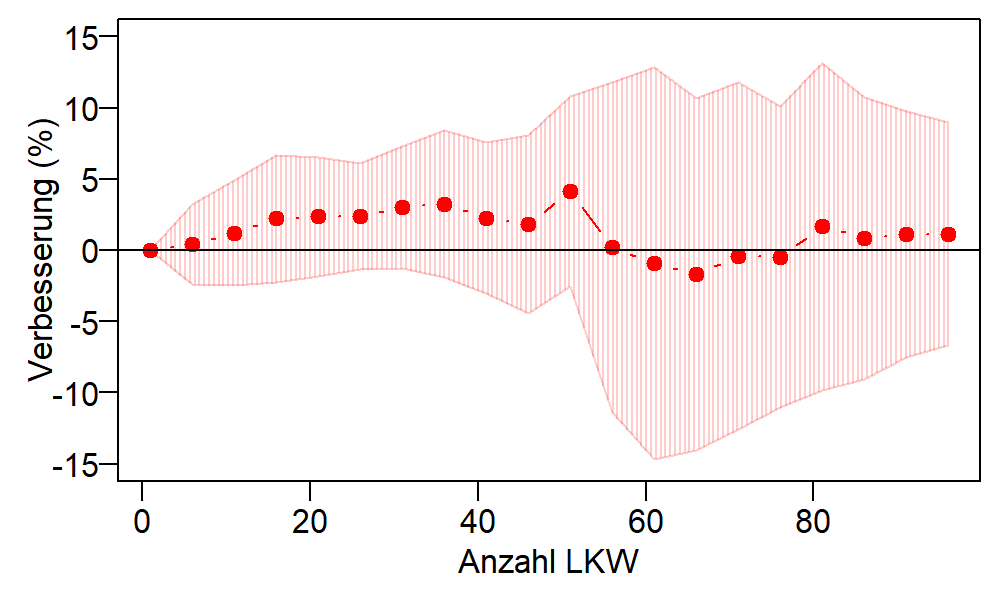
\includegraphics[width=\linewidth]{images/graphs/rsNumberOfTrucksSjn_AnzahlAbgefertigt.png}
  \caption{Shortest Job Next}
  \label{fig:eal1}
\end{subfigure}
\begin{subfigure}{.495\textwidth}
  \centering
  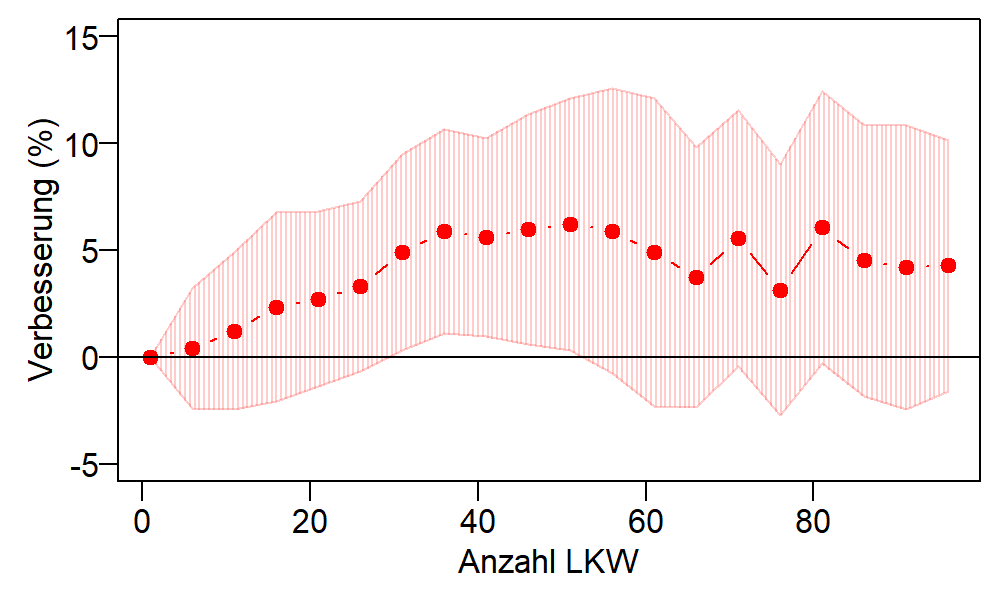
\includegraphics[width=\linewidth]{images/graphs/rsNumberOfTrucksMot_AnzahlAbgefertigt.png}
  \caption{Most Idle Time}
  \label{fig:eal2}
\end{subfigure}

\begin{subfigure}{.5\textwidth}
  \centering
  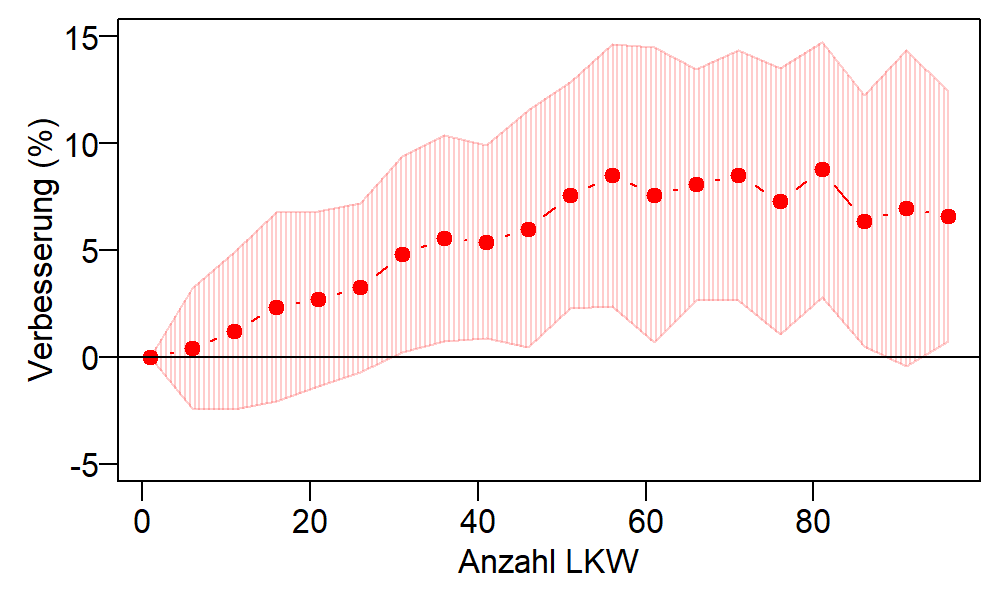
\includegraphics[width=\linewidth]{images/graphs/rsNumberOfTrucksFcfs_AnzahlAbgefertigt.png}
  \caption{First come, first served}
  \label{fig:eal3}
\end{subfigure}

\caption{Verbesserung der Anzahl abgefertigter LKW}
\label{fig:evalAnzahlLkw}
\end{figure}

Was zunächst einmal bei allen Algorithmen auffällig ist, ist dass die Standardabweichung, also die Streuung der Werte sehr hoch ist. Hier ist jeweils die einfache Standardabweichung dargestellt, d.h. geht man von einer Normalverteilung der Werte aus, so liegen in den rot schraffierten Bereichen 68\% der Werte. Eine doppelte Standardabweichung mit 95\% der Werte würde also bei allen Algorithmen im negativen Bereich liegen. Kein Algorithmus garantiert also eine Verbesserung der Werte. Ebenfalls ist bei allen Graphen eine stark sichtbare Veränderung des Anstiegs zwischen 40 und 60 LKW zu erkennen. Dies dürfte etwa die Grenze sein, bei der der 180 Minuten Slot vollgefüllt ist. Bis dort hin bleibt so viel Leerlauf, dass die meisten LKW noch eingeplant werden können, ab dann können die meisten neuen LKW nicht mehr eingeplant werden. Alle Graphen zeigen auch bis etwa 30 LKW eine ähnlich starke Verbesserung von ca. 4-5\%, was darauf zurückzuführen ist, dass in diesem Bereich immer nahezu alle LKW eingeplant werden können und keiner verschoben werden muss.

Auffällig in Graph \ref{fig:eal1} für das Shortest Job Next Verfahren ist allerdings, dass es eine deutlich geringere Verbesserung bei insgesamt größerer Streuung gibt. Bis der Slot bei etwa 50 LKW gefüllt ist, gibt es durchschnittlich eine leichte Verbesserung bis zu etwa 3\%. Die Streuung ist dabei sogar leicht geringer als bei den anderen Algorithmen. Danach fällt die Verbesserung allerdings stark ab und pendelt um 0 herum, teilweise sogar leicht ins negative bei extremer Streuung. Schaut man sich beispielhaft eine grafische Darstellung der Verteilung an (siehe Abb. \ref{}\todo{Beispiel einfügen}), so fällt auf, dass durch die Verplanung der kurzesten Aufgaben am Anfang eine starke Ungleichverteilung entsteht. Zumindest bei den hier gewählten Ladezeiten haben immer die gleichen Abfertigungskategorien auch die kürzesten Ladezeiten, sodass immer die gleichen Ressourcen genutzt werden und im Anschluss andere kaum mehr verplant werden können, weil sie oft parallel mit bereits verplanten Ressourcen vorkommen.

Im Planungsverfahren mit der meisten Leerlaufzeit (siehe Graph \ref{fig:eal2}) lässt sich eine deutlichere Verbesserung erkennen. Bis zur Füllung des Slots bei etwa 40 LKW gibt es eine kontinuierliche Verbesserung bis zu ca. 5\%, bei moderater Streuung. Anschließend pendelt sich die Verbesserung bei 5\% ein, bei allerdings deutlich steigender Streuung. Die anfängliche Steigung dürfte damit zusammen hängen, dass es mit wenigen LKW einfach auch nur möglich ist eine geringe Verbesserung zu erzielen. Je mehr LKW kommen, desto mehr Potenzial kann auch ausgeschöpft werden.

Bei der first come, first served Verteilung (siehe Graph \ref{fig:eal3}) ergibt sich ein sehr ähnliches Bild wie in Graph \ref{fig:eal2}. Bis etwa 40 LKW sind die Steigung und auch die Streuung sehr ähnlich. Allerdings geht die Steigung hier noch bis eta 50 LKW und 7-8\% Verbesserung weiter. Erst dann stagniert diese ebenfalls auch etwa gleichbeibender Höhe und deutlich steigender Streuung.

Bezüglich der Anzahl der möglichen Abfertigungen lässt sich aus dieser Betrachtung schließen, dass die Algorithmen MIT und FCFS für den allgemeinen Fall deutlich besser geeignet sind. Die große Streuung zeigt allerdings auch, dass es sehr große Unsicherheiten bei allen Algorithmen gibt. Dies dürfte vor allem mit der Zufälligkeit der Eingabewerte zusammenhängen. Wenn kaum etwas über die Verteilung der ankommenden LKW bekannt ist, ist es sehr schwierig einen spezialisierten Algorithmus zu finden. Somit kann nur auf allgemein funktionierende Verfahren zurückgegriffen werden, welche dann in der Regel auch Verbesserte Werte liefern. Was allerdings positiv zu bemerken ist, ist dass genau der Wendepunkt zu dem die Slots gefüllt sind, auch der Hochpunkt der Verbesserung ist. Es ergibt aus dieser Betrachtungsweise somit kaum Sinn, Überbuchungen und anschließende Verschiebung einiger LKW in andere Slots vorzunehmen, da es kaum noch Verbesserung bei der Anzahl der verarbeiteten LKW gibt.


\textbf{Verbesserung der Leerlaufzeiten der Ressourcen}

Die Leerlaufzeit der Ressourcen ist, wie erwähnt, ebenfalls von Bedeutung. Je weniger ungenutzte Leerlaufzeit eine Ressource innerhalb des Slots hat, desto mehr wird sie produktiv und wirtschaftlich sinnvoll eingesetzt. Auch hier ist als relatives Maß die prozentuale Verbesserung zwischen den jeweils unoptimierten und optimierten Zeiten aufgetragen. Berechnet wurden diese nach den Formeln \ref{eq:idleImpr} und \ref{eq:idleBestJobsImpr}. Da die Leerlaufzeit bereits in Prozent gespeichert wird, reicht hier die Darstellung der Differenz, um die Verbesserung zu sehen.

\begin{equation} \label{eq:idleImpr}
idleImpr = uIdleTotal - oIdleTotal
\end{equation}
%\begin{equation} \label{eq:idleCompleteImpr}
%idleCompleteImpr = uIdleComplete - oIdleComplete
%\end{equation}
\begin{equation} \label{eq:idleBestJobsImpr}
idleBestJobsImpr = uIdleBetweenJobs - oIdleBetweenJobs
\end{equation}

Die Graphen stellen hier jeweils die Verbesserungen der gesamten Leerlaufzeit, der Leerlaufzeit und die Leerlaufzeit zwischen den einzelnen Jobs dar.

\begin{figure}[H]
\centering
\begin{subfigure}{.495\textwidth}
  \centering
  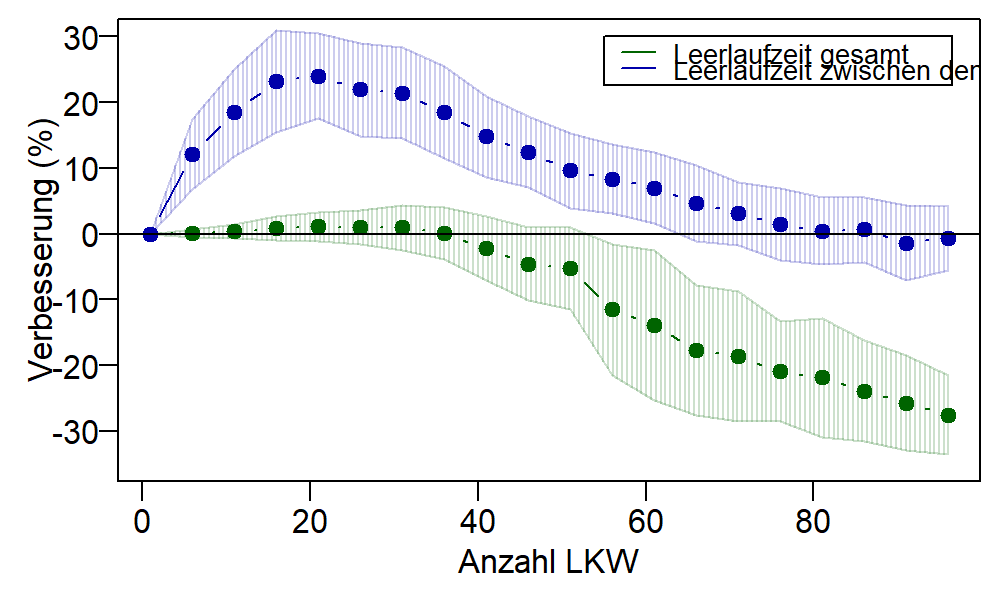
\includegraphics[width=\linewidth]{images/graphs/rsNumberOfTrucksSjn_Leerlaufzeit.png}
  \caption{Shortest Job Next}
  \label{fig:el1}
\end{subfigure}
\begin{subfigure}{.495\textwidth}
  \centering
  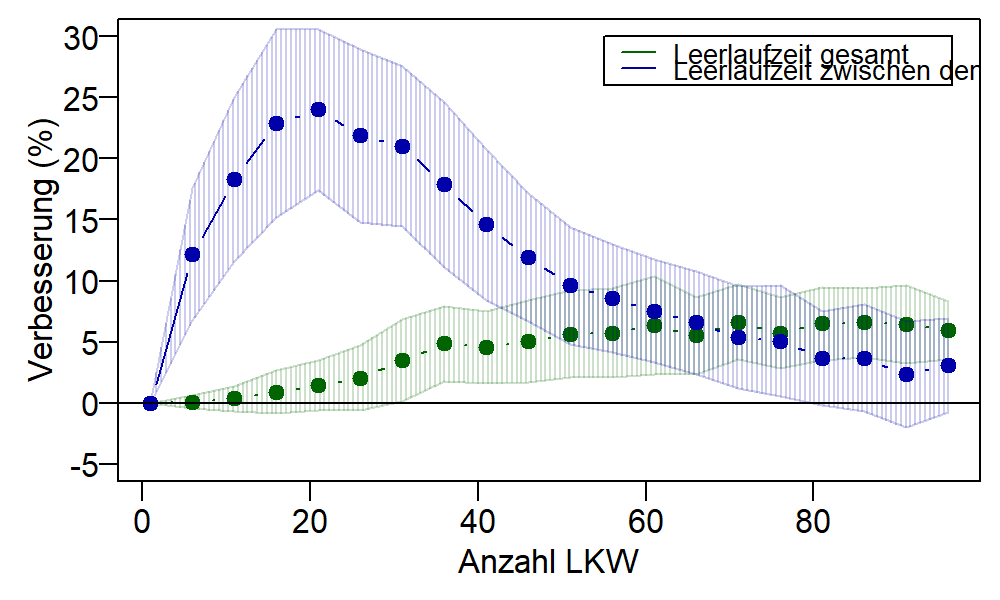
\includegraphics[width=\linewidth]{images/graphs/rsNumberOfTrucksMot_Leerlaufzeit.png}
  \caption{Most Idle Time}
  \label{fig:el2}
\end{subfigure}

\begin{subfigure}{.5\textwidth}
  \centering
  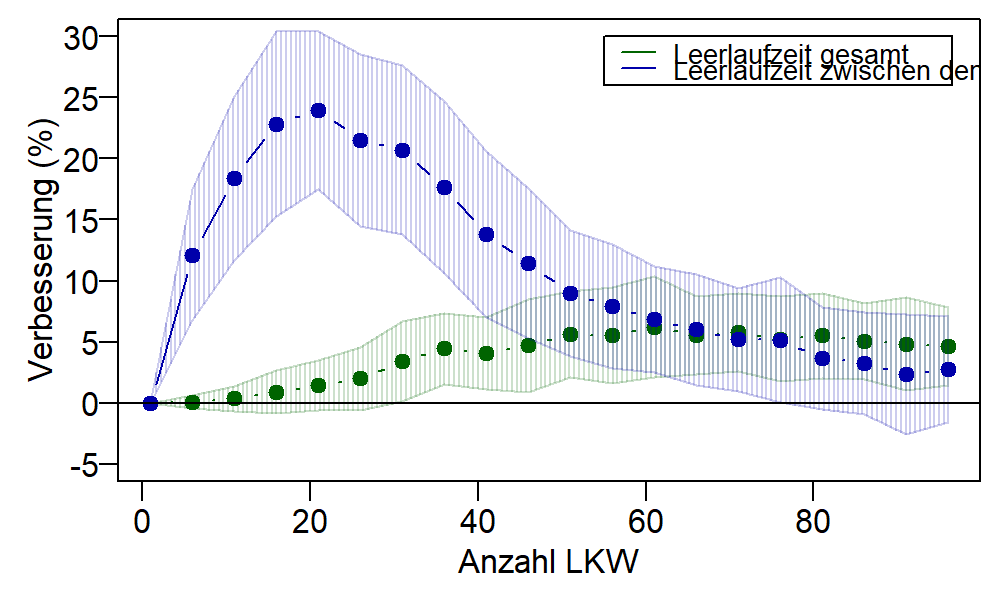
\includegraphics[width=\linewidth]{images/graphs/rsNumberOfTrucksFcfs_Leerlaufzeit.png}
  \caption{First come, first served}
  \label{fig:el3}
\end{subfigure}

\caption{Verbesserung der Leerlaufzeiten der abgefertigten LKW}
\label{fig:evalLeerlaufzeit}
\end{figure}

Mit Blick auf die Leerlaufzeiten lässt sich feststellen, dass die Streuungen hier zwar vorhanden, aber deutlich geringer sind. In den meisten Fällen ergeben sich so keine negativen Verbesserungen bzw. Verschlechterungen der Werte.

In Bezug auf die Leerlaufzeiten schneidet das SJN Verfahren allerdings auch nicht besonders gut ab (siehe Graph \ref{fig:el1}). Die Leerlaufzeiten zwischen den Aufträgen verzeichnen hier zwar eine deutliche Verbesserung von im maximalen Durchschnitt etwa 25\%. Auch die Standardabweichung bis etwa 50-60 LKW so gering, dass es hier so gut wie durchgängig Verbesserungen gegenüber dem unoptimierten Fall gibt. Die Gesamtleerlaufzeit über den Slot verbessert sich allerdings zu Beginn nur ganz minimal und dann zwar auch nur mit sehr geringer Streuung, allerdings verschlechtert sich diese nach dem Füllen des Slots sehr rapide bis zu etwa -25\% bei 100 LKW und einer größer werdenden Streuung. Erklären lässt sich dies in Kombination mit der Anzahl der abgefertigten LKW (siehe Graph \ref{fig:eal1}). Bis der Slot gefüllt ist, lassen sich unoptimiert wie optimiert so gut wie alle LKW unterbringen, somit ergibt sich dort wenig Vorteil bei der Leerlaufzeit. Danach allerdings werden im Durchschnitt gar keine zusätzlichen LKW eingeplant, dafür werden allerdings nach dem Shortest Job Next Prinzip nur die kurzen Aufgaben verplant und die langen fallen heraus und müssen verschoben werden. Insgesamt entsteht aber so eine geringere Auslastung der Ressourcen und somit eine deutliche Verschlechterung, die auch immer weiter ansteigt, je mehr kurze Aufträge es gibt.

Die Verfahren MIT und FCFS unterscheiden sich im direkten Vergleich nur sehr minimal (siehe Graphen \ref{fig:el2} und \ref{fig:el3}). Beide zeigen über den ganzen Zeitraum eine deutlich positive Verbesserung der Leerlaufzeit zwischen den LKW. Diese steigt bis im Durchschnitt etwa 25\% bei 20 LKW an und nimmt dann wieder ab. Um den Bereich zwischen 50 und 60 LKW, wo der Slot wieder komplett ausgefüllt wird, verlangsamt sich diese Abnahme, bleibt aber weiter positiv. Auch unter Berücksichtigung der Standardabweichung ist diese Verbesserung in nahezu allen Fällen positiv. Auch die Gesamtleerlaufzeit lässt eine gute Verbesserung erkennen. Bis etwa 6\% bei 60 LKW steigt diese Zeit bei beiden kontinuierlich an und hält sich dann auf etwa gleichbleibendem Niveau. Die Standardabweichung ist dabei zunächst sehr gering und wird dann bis zum höchsten Niveau immer größer. De größte Teil aller Werte liegt dabei aber immer noch im positiven Bereich, wenn auch deultich geringer als der Durchschnitt.

Schlussfolgern kann man aus dieser Betrachtung, dass das SJN Verfahren zwar für die Verplanung einzelner Ressourcen bezüglich der Leerlaufzeit Vorteile bringt, da die Zeiten zwischen den Ressourcen minimiert werden, über alle Ressourcen betrachtet ergibt sich allerdings kein Vorteil bzw. sogar ein starker Nachteil. Es werden nur kürzere und dabei aber auch nicht mehr Aufträge verplant. Dies bringt nicht nur hier Nachteile, die verschobenen Jobs müssen in späteren Slots zusätzlich eingeplant werden, was dort ebenfalls für große Schwierigkeiten und eine Ungleichverteilung der Auslastungen sorgen wird. Die beiden anderen Verfahren können dagegen allerdings den psoitiven Eindruck der vorherigen Auswertung bestätigen. Bei mehr eingeplanten LKW kann hier gleichzeitig eine geringere Leerlaufzeit verzeichnet werden. Der große Vorteil im Vergleich zu SJN dürfte sein, dass bei beiden Verfahren mehr oder weniger zufällig über alle Abfertigungskategorien hinweg aus den Aufträgen ausgewählt wird. Somit werden die Ressourcen im Schnitt gleichmäßiger ausgelastet und das strukturierte Vorgehen bei der Verteilung kann dann weniger Leerlauf schaffen und so zusätzliche LKW einsetzen.



\textbf{Verbesserung der Wartezeiten je LKW}

Ein Wert, welcher nicht direktes Ziel der Verbesserung war, aber dennoch interessant für eine nähere Betrachtung ist, ist die Entwicklung der Wartezeit der LKW. Lassen sich LKW schneller zu Beginn abarbeiten, kann dies ein Vorteil sein, da LKW Fahrer so nicht so lange ungenutzte Wartezeiten vor oder im Terminal haben und schneller für ihre Speditionen neue Aufträge bearbeiten können.

\begin{equation} \label{eq:avgWaitingImpr}
avgWaitingImpr = \dfrac{uAverageWaitingTime - oAverageWaitingTime}{uAverageWaitingTime} * 100
\end{equation}

\begin{figure}[H]
\centering
\begin{subfigure}{.495\textwidth}
  \centering
  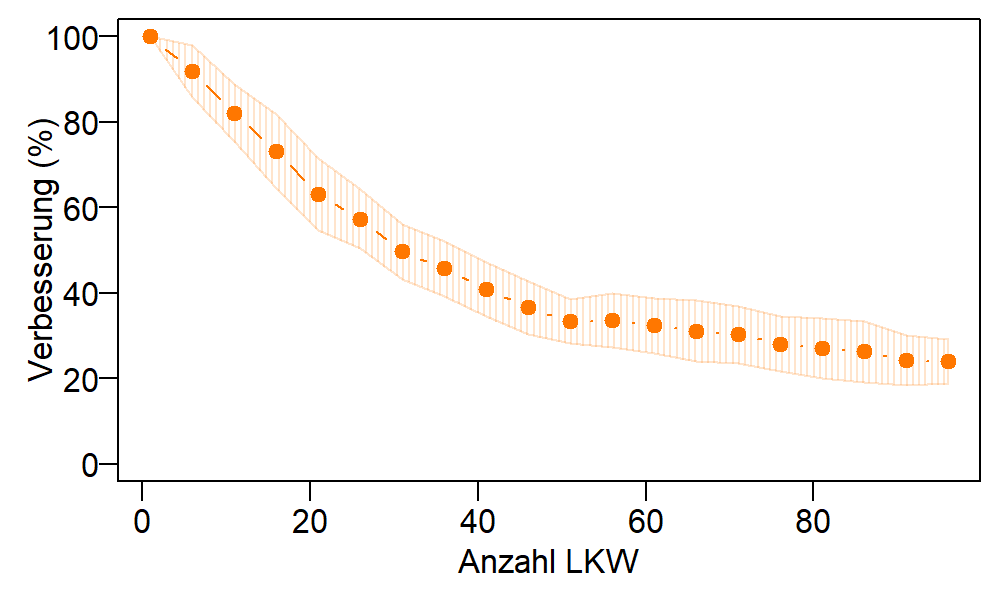
\includegraphics[width=\linewidth]{images/graphs/rsNumberOfTrucksSjn_Wartezeit.png}
  \caption{Shortest Job Next}
  \label{fig:ew1}
\end{subfigure}
\begin{subfigure}{.495\textwidth}
  \centering
  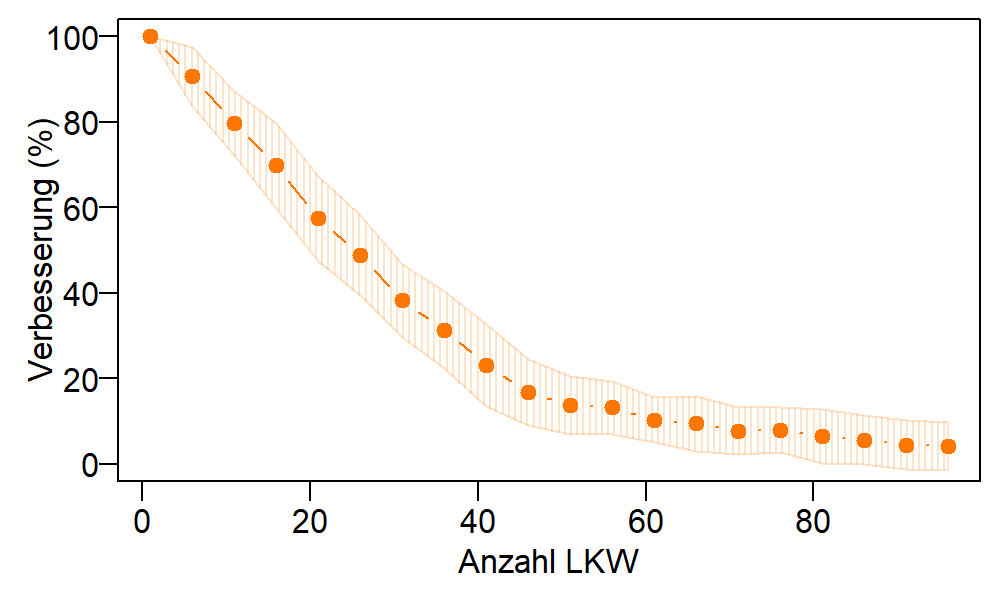
\includegraphics[width=\linewidth]{images/graphs/rsNumberOfTrucksMot_Wartezeit.png}
  \caption{Most Idle Time}
  \label{fig:ew2}
\end{subfigure}

\begin{subfigure}{.5\textwidth}
  \centering
  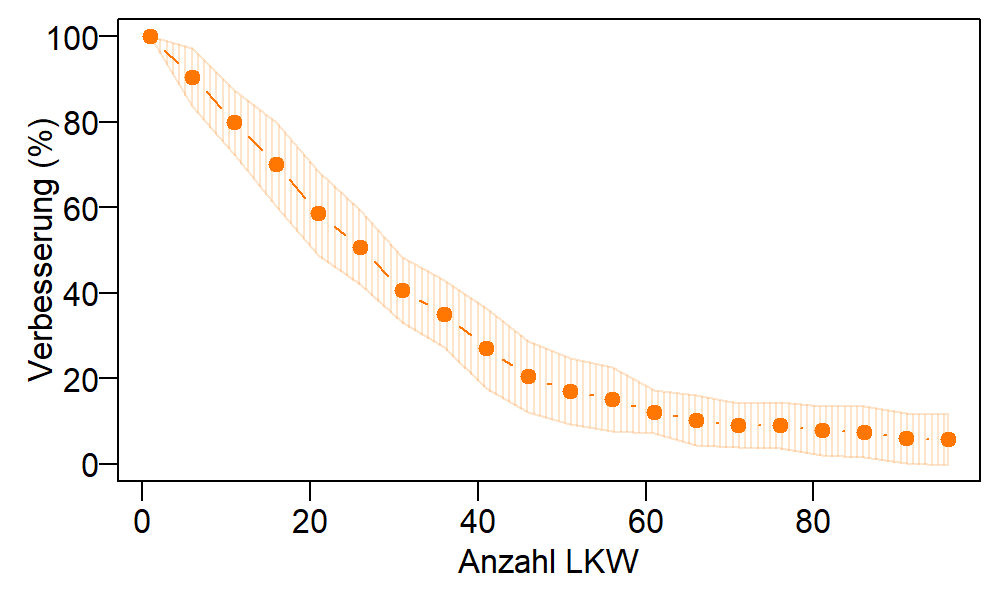
\includegraphics[width=\linewidth]{images/graphs/rsNumberOfTrucksFcfs_Wartezeit.png}
  \caption{First come, first served}
  \label{fig:ew3}
\end{subfigure}

\caption{Verbesserung der Wartezeit der abgefertigten LKW}
\label{fig:evalWartezeit}
\end{figure}

Bei den Wartezeiten ergibt sich ein etwas anderes Bild der betrachteten Verfahren. Alle beginnen bei einer Verbesserung der Wartezeit von 100\%, welche dann überall deutlich sinkt, bis zu dem Punkt wo wieder der gesamte Slot gefüllt ist. Ab diesem Punkt sinkt die Wartezeit überall weiter, allerdings deutlich langsamer. Auch die Streuung ist in diesem Fall sehr gering, sodass es keine Verschlechterungen der Wartezeit gibt.  Die anfänglich sehr große Verbesserung lässt sich darauf zurückführen, dass die LKW im unoptimierten Fall sehr zufällig verteilt über den gesamten Zeitraum des Slots ankommen. So wird jedes Planungsverfahren, welches die Aufgaben so früh wie möglich einplant, zunächst eine deutliche Verbesserung erreichen.

Auffällig ist vor allem, dass die Wartezeit den SJN Verfahrens (siehe Graph \ref{fig:ew1}) langsamer sinkt und sich auch am Ende noch auf einem Niveau von 30-40\% Verbesserung bewegt, während die anderen beiden Fälle (siehe Graphen \ref{fig:ew2} und \ref{fig:ew3}) wieder sehr ähnlich sind und gegen Ende nur noch eine Verbesserung von 10-20\% haben. Dies ist daraum zurückzuführen, dass das SJN Verfahren alle kurzen Aufgaben zuerst einplant, somit können schnell viele LKW abgearbeitet werden, was zu wenig Wartezeit führt. Spätestens, wenn der Slot komplett gefüllt ist und LKW verschoben werden müssen, wird sich der Vorteil dadurch relativieren, dass die verschobenen LKW mit langer Abfertigungszeit in anderen Slots untergebracht werden müssen und damit dort die Wartezeit negativ beeinflussen.

Insgesamt lässt sich aber festhalten, dass in allen Verfahren eine, wenn auch nicht immer allzu hohe Verbesserung erzielt werden kann. Dies war zwar nicht oberstes Ziel der Optimierung, ist allerdings ein schöner und für die LKW Fahrer und Speditionen vorteilhafter Nebeneffekt.



\subsubsection{Testszenario 2: Verhalten bei Überbuchung}

Ein weitere Betrachtungsweise der Algorithmen ist das Verhalten mit zunehmender Anzahl von Buchungen. In diesem Fall wird eine gleichbleibende Liste von Buchungen genutzt, welcher schrittweise LKW hinzugefügt werden. Dies simuliert, dass sich immer weitere LKW Fahrer einen Slot buchen. Interessant ist hier, wie viel Verbesserung sich erzielen lässt, wenn bis zur Auslastungsgrenze des Slots gebucht werden würde und alle weiteren, nicht mehr passenden LKW abgewiesen, bzw. diesen nur noch andere Slots zu Buchung vorgeschlagen werden. Dagegen wäre die Frage, wie viele Überbuchungen man zulassen könnte. Hier würden dann zunächst mehr LKW angenommen, als schaffbar sind. Der Planungsalgorithmus kann dann die für ihn passenden Buchungen nutzen und die restlichen in den nächsten Slot verschieben. Es wurden hier sehr ähnliche Berechnungen, wie im vorherigen Testszenario angewendet, auch hier wird ein Vergleich von simulierten, unoptimierten Zustand zu den Ergebnissen der verschiedenen Algorithmen vorgenommen.

Die Werte der folgenden Auswertung wurden durch die Testklasse \textit{OverfillTest} erzeugt. Alle anschließenden Berechnungen und Graphen sind mit dem R Skript \textit{rsOverfill.R}\todo{Pfad etc} berechnet worden.

Die Graphen (Abb. \ref{fig:evalOverfill}) zeigen in diesem Fall jeweils die absolute Anzahl an tatsächlich geplanten LKW im unoptimierten Zustand (blau) und im optimierten Fall (rot). So ist in hier deutlicher erkennbar, wann nicht mehr alle LKW eingeplant werden können, wann also Überbuchungen stattfinden müssten. Die diagonale Gerade mit einer Steigung von 1 zeigt dabei den Fall eines unbegrenzten Slots, sodass jeder LKW, welcher gebucht wurde auch verarbeitet werden kann. Im Verhältnis dazu wird auf der zweiten y-Achse die Verbesserung der Leerlaufzeit aufgetragen. Die Zeit zwischen den LKW in orange und die Gesamtleerlaufzeit in grün. Diese wurden wieder nach dem gleichen Weg wie im ersten Testszenario berechnet (siehe Formeln \ref{eq:idleImpr} und \ref{eq:idleBestJobsImpr}). So lässt sich ein direkter Vergleich anstellen, bei wie viel Buchungen die effektivste Ausnutzung des Slots erreicht wird.


\begin{figure}[H]
\centering
\begin{subfigure}{.495\textwidth}
  \centering
  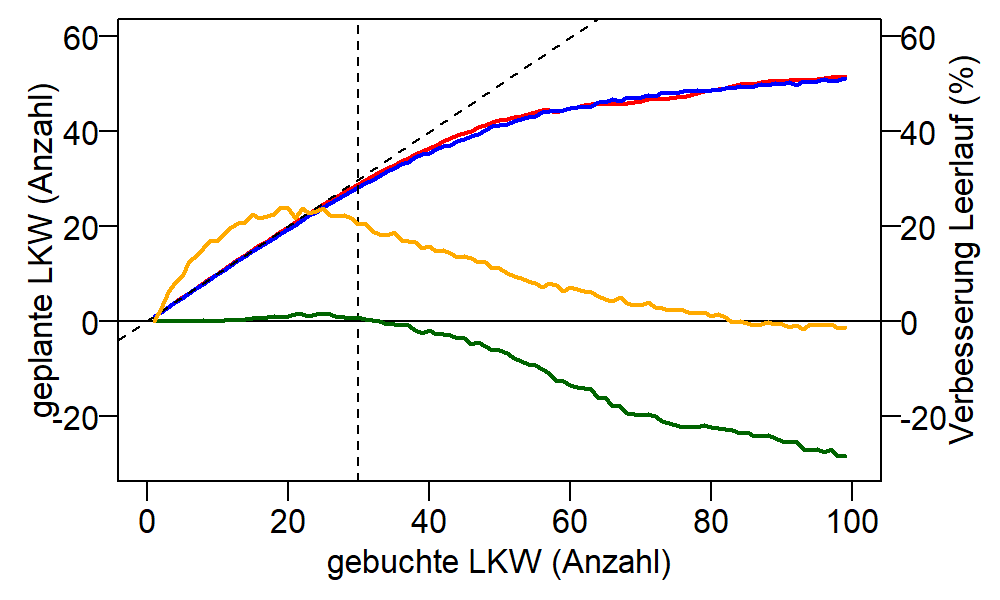
\includegraphics[width=\linewidth]{images/graphs/rsOverfillSjn.png}
  \caption{Shortest Job Next}
  \label{fig:eof1}
\end{subfigure}
\begin{subfigure}{.495\textwidth}
  \centering
  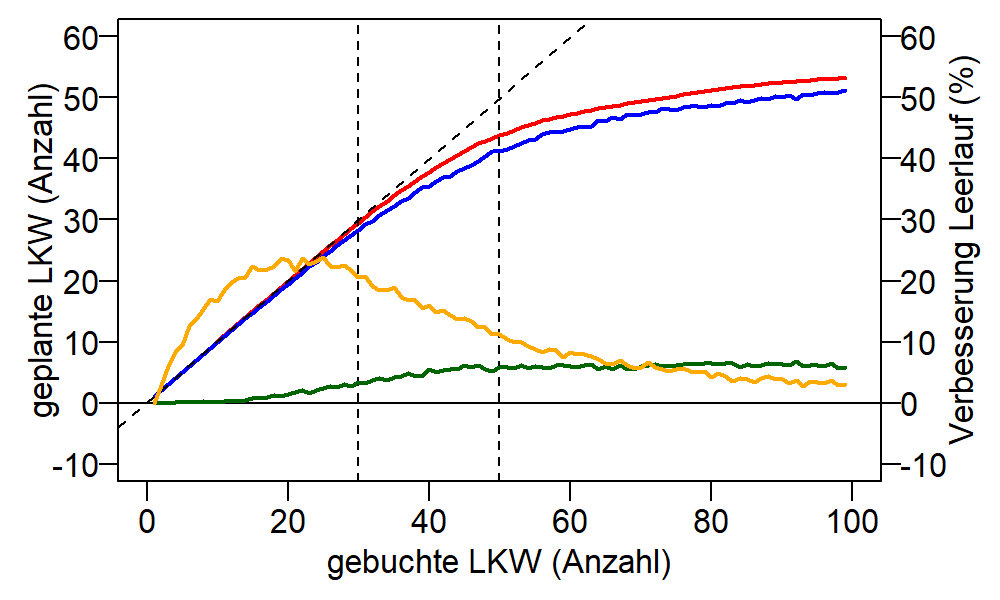
\includegraphics[width=\linewidth]{images/graphs/rsOverfillMit.png}
  \caption{Most Idle Time}
  \label{fig:eof2}
\end{subfigure}

\begin{subfigure}{.5\textwidth}
  \centering
  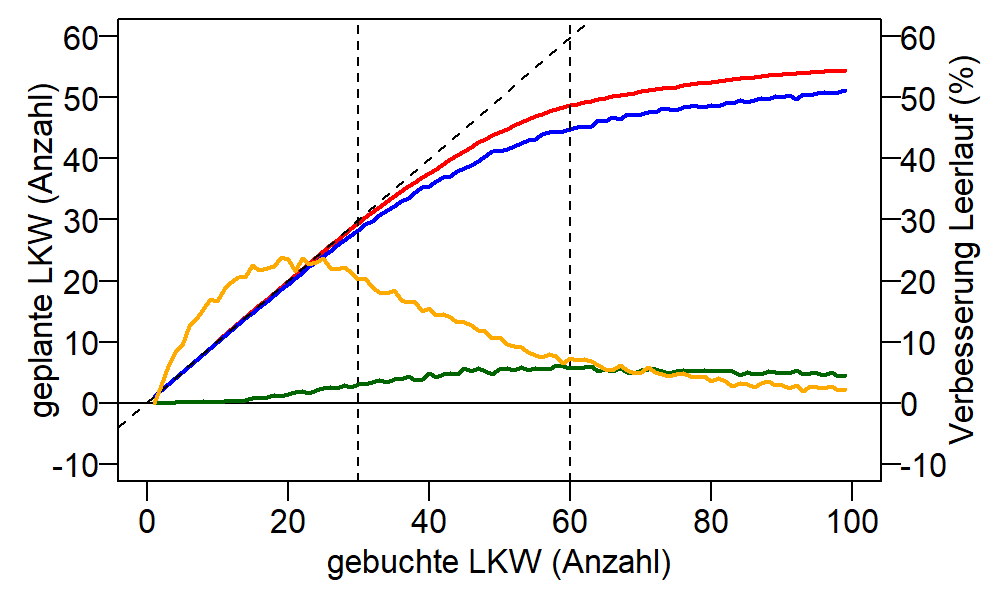
\includegraphics[width=\linewidth]{images/graphs/rsOverfillFcfs.png}
  \caption{First come, first served}
  \label{fig:eof3}
\end{subfigure}
\caption{Verhalten bei Überbuchung}
\label{fig:evalOverfill}
\end{figure}
\todo{Zuklein?, Legende?!}

Erkennbar ist zunächst einmal bei allen Darstellungen, dass überall die Anzahl der eingeplanten LKW bei etwa 30 anfängt, von der diagonalen für den unbegrenzten Slot abweicht. Dies ist also bei allen der Punkt, wo im Durchschnitt langsam nicht mehr alle LKW in den Slot passen. Verdeutlicht wird dieser Punkt in allen Graphen durch die erste senkrechte Linie.

Im SJN Verfahren (siehe Graph \ref{fig:eof1}) halten sich die beiden Anzahlen der eingeplanten LKW sehr nah beieinander, es gibt also im Durchschnitt kaum Verbesserungen oder Verschlechterungen. Die Gesamtleerlaufzeit verschlechtert sich ganz zu Beginn leicht und Verbessert sich dann bis zur markanten Grenze von 30 LKW leicht. Anschließend fällt sie rapide ab, wie es auch schon im vorherigen Szenario sichtbar war. Fängt man hier also an zu überbuchen, werden im Durchschnitt nicht mehr LKW abgefertigt, dafür steigt aber die Leerlaufzeit massiv. 

Auch in diesem Beispiel wiesen die Graphen der Verfahren MIT und FCFS (Abb. \ref{fig:eof2} und \ref{fig:eof3}) deutliche Ähnlichkeiten auf. Hier lässt sich allerdings ab 30 LKW ein größerer Anstieg der geplanten LKW im optimierten Fall erkennen, als es unoptimiert der Fall ist. Auffällig ist aber, dass die Steigung bei MIT schon bei etwa 50 LKW anfängt, deutlicher zu sinken, während es im FCFS Verfahren erst bei etwa 60 LKW der Fall ist (vgl. die zweite senkrechte Linie in den jeweiligen Graphen). Dies ist auch jeweils der Punkt, wo der Abstand zwischen der roten und der blauen Linie nicht mehr größer wird und somit auch kaum noch eine Verbesserung in der Anzahl der abgefertigten LKW stattfindet. Gleichzeitig ist dies auch der Punkt, an dem die Steigung bei der Verbesserung der Gesamtleerlaufzeit stagniert. Auch die Verbesserung Leerlaufzeit zwischen den den Aufträgen nähert sich ab da der Null an. 

Für die beiden Planungsverfahren MIT und FCFS kann man also festhalten, dass gewisse Überbuchung durchaus von Vorteil ist. Für den dreistündigen Slot, welcher ohne Überbuchung schon bei ca. 30 LKW gefüllt wäre, kann man durchaus eine Überbuchung im Bereich von 50-100\%, also insgesamt 45 bis 60 LKW zulassen. Dies führt zu einer deutlich optimierten Auslastung des Slots. Während im SJN Verfahren eine Verschiebung bedeuten würde, dass auch in nachfolgenden Slots eine Ungleichverteilung stattfinden würde, würde sich eine Verschiebung hier vermutlich nicht wirklich negativ auswirken. Da die Verteilung der Abfertigungskategorien, wie bereits festgestellt, ohnehin sher gleichmäßig ist, würde auch eine gleichmäßig durchmischte Liste verschoben. Darüber hinaus lässt sich eben bei einer Überbuchung eine deutlich verbesserte Auslastung und verringerte Leerlaufzeit erzielen, welche bei strikter Begrenzung der Buchungen sehr sehr viel geringer ausfallen wird.


\subsubsection{Testszenario 3: Verhalten bei unterschiedlicher Slotgröße}
\todo{Leerlaufzeit vergleichen?}

In diesem Test soll nun im Gegensatz zu den Vorherigen die Slotgröße variiert werden. Die bisherige Größe wurde mit 180 Minuten gewählt, da sich so eine höhere Anzahl und \glqq{}Auflösung\grqq{} bei den gebuchten LKW ergibt. Bei sehr kleinen Slots lassen sich noch weniger signifikante Veränderungen bis zur Slotsgrenze darstellen, wie auch der folgende Test zeigt. \todo{Ist das wirklich so, prüfen, wenn geschrieben...} Zu analysieren ist hier, wie sich die Anzahl der geplanten LKW und die Leerlaufzeiten verbessern, wenn kleinere oder größere Slots verwendet werden. Dies ist auch für den realen Einsatz sehr interessant, um das beste Verhältnis zwischen möglichst guter Optimierung und den Bedürfnissen der LKW Fahrer und Speditionen zu finden.

Die Werte für dieses Szenario wurden mit den Implementierungen aus der Testklasse \textit{SlotsizeTest} berechnet. Mit dem R Skript \textit{rsSlotsize.R} \todo{Pfad etc.} wurden alle Graphen und Berechnungen erzeugt.

Dargestellt werden in den Auswertungen jeweils wieder die prozentuale Verbesserung bei der Anzahl der eingeplanten LKW. Zur Berechnung wurde wieder die Formel \ref{eq:schedJobImpr} genutzt. Dabei entspricht jede Linie einer anderen Slotgröße.

\begin{figure}[H]
\centering
\begin{subfigure}{.495\textwidth}
  \centering
  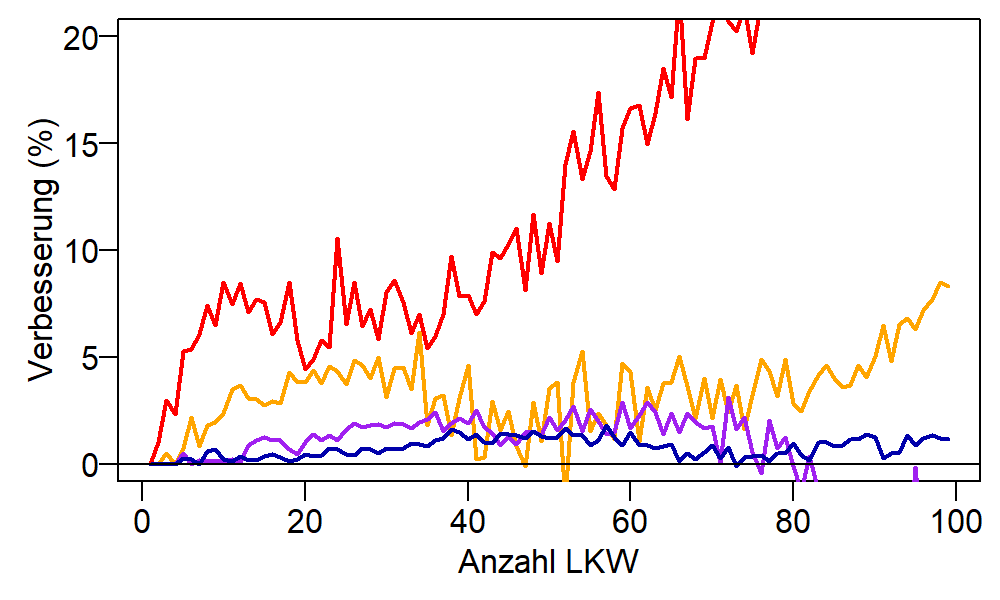
\includegraphics[width=\linewidth]{images/graphs/rsSlotsizeSjn.png}
  \caption{Shortest Job Next}
  \label{fig:eof1}
\end{subfigure}
\begin{subfigure}{.495\textwidth}
  \centering
  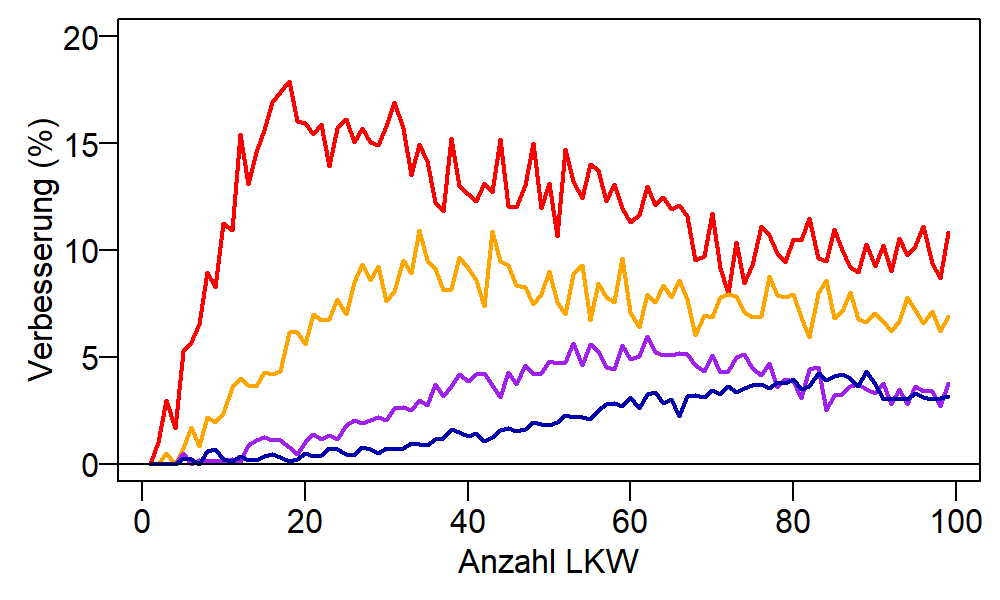
\includegraphics[width=\linewidth]{images/graphs/rsSlotsizeMit.png}
  \caption{Most Idle Time}
  \label{fig:eof2}
\end{subfigure}

\begin{subfigure}{.5\textwidth}
  \centering
  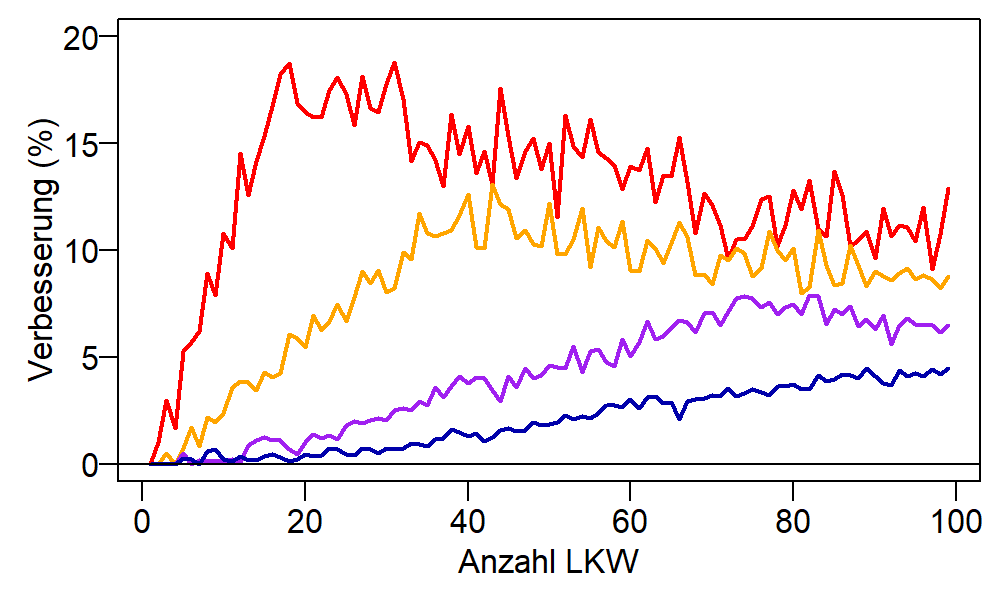
\includegraphics[width=\linewidth]{images/graphs/rsSlotsizeFcfs.png}
  \caption{First come, first served}
  \label{fig:eof3}
\end{subfigure}
\caption{Verbesserung der geplanten LKW bei veränderter Slotgröße}
\label{fig:evalSlotsize}
\end{figure}
\todo{Zuklein?, Legende?!, evtl. auch nicht Verbesserung sondern oScheduled zeigen, wegen streuung?!}

\begin{figure}[H]
\centering
\begin{subfigure}{.495\textwidth}
  \centering
  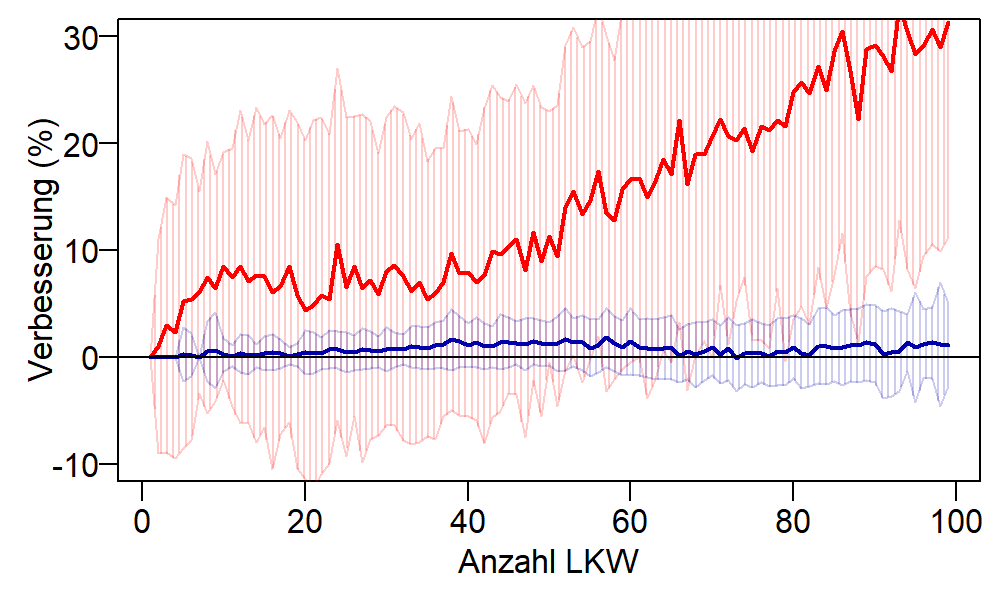
\includegraphics[width=\linewidth]{images/graphs/rsSlotsizeSjn_Streuung.png}
  \caption{Shortest Job Next}
  \label{fig:eofs1}
\end{subfigure}
\begin{subfigure}{.495\textwidth}
  \centering
  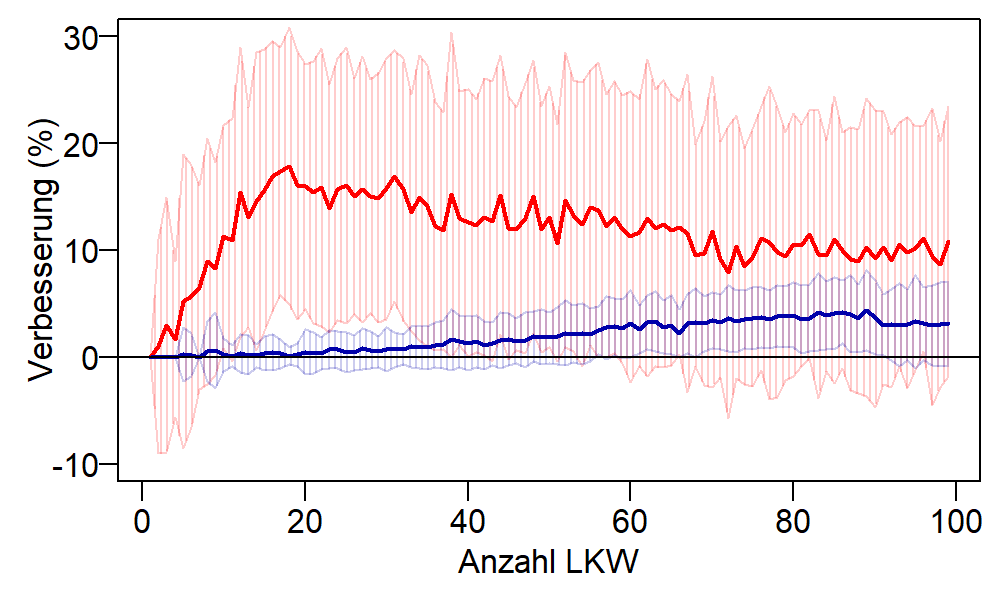
\includegraphics[width=\linewidth]{images/graphs/rsSlotsizeMit_Streuung.png}
  \caption{Most Idle Time}
  \label{fig:eofs2}
\end{subfigure}

\begin{subfigure}{.5\textwidth}
  \centering
  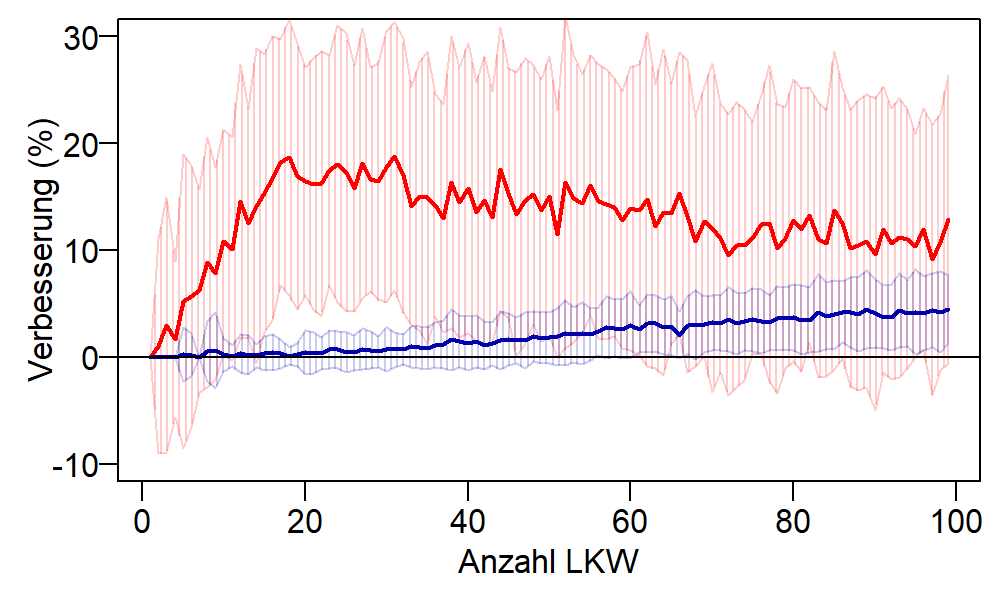
\includegraphics[width=\linewidth]{images/graphs/rsSlotsizeFcfs_Streuung.png}
  \caption{First come, first served}
  \label{fig:eofs3}
\end{subfigure}
\caption{Streuung der Verbesserung der geplanten LKW bei veränderter Slotgröße}
\label{fig:evalSlotsizeStreuung}
\end{figure}
\todo{Zuklein?, Legende?!}

Eine Betrachtung der Testergebnisse (siehe Abb. \ref{fig:evalSlotsize}) zeigt hier tatsächlich unerwartet große Unterschiede auf. In der Gesamtsicht lässt sich schon auf den ersten Blick fetsthalten, dass eine Veränderung der Slotgröße erheblichen Einfluss auf die Verbesserungsrate hat. 

Der Eindruck, dass das SJN Verfahren eher keine allzu guten Ergebnisse liefert, setzt sich hier fort. Die Streuung der Werte ist sehr hoch, insbesondere bei kleinen Slots (siehe Graphen \ref{fig:evalSlotsizeStreuung}). Bei 60 Minuten Slotgröße ist noch eine relativ hohe Verbesserung zwischen 5 und 10\% zu erkennen, welche ab ca. 40 LKW auch noch einmal extrem weiter ansteigt. Je größer die Slots allerdings werden, desto geringer oder sogar negativer wird die Verbesserung. Man könnte nun sagen, dass die Verbesserung beim 60 Minuten Slot wirklich gut ist. Allerdings wurde in den vorherigen Szenarien bereits festgestellt, dass sich eine Überbuchung insgesamt sehr negativ auswirkt. Der extreme Anstieg der Verbesserung kann also gar nicht genutzt werden, da nur die ersten 10-15 LKW wirklich sinnvoll eingeplant werden können. Alle weitere Verbesserung ist nicht nutzbar, da so extrem viele LKW auf andere Slots verschoben werden müssten und sind dann dort sehr negativ auswirken. Auch die hohe Streuung der Werte sprich nicht gerade für ein gutes Verfahren, da kaum konstant positive Ergebnisse erzeugt werden.

Anders sieht es dagegen wieder bei den beiden anderen Verfahren aus. Auch hier lassen sich wieder große Ähnlichkeiten zwischen den Auswertungen der beiden Verfahren feststellen. In allen Kurven ist ein starker Anstieg bis zu einem Maximum zu erkennen und ein anschließender, leichterer Abfall der Verbesserung. Diese Spitze verschiebt sich mit steigender Größe der Slots nach hinten, was auf die größere Kapazität für LKW zurückzuführen ist. Sehr auffällig ist, dass es bei kleineren Slots deutlich höheres Verbesserungspotenzial gibt. Im 60 Minuten Slot erreicht das MIT Verfahren im Durchschnitt bis zu ca. 17\% Verbesserung und das FCFS Verfahren sogar noch mit durchschnittlich etwa 18\% in der Spitze sogar noch etwas mehr. Im 120 Minuten Slot sind es nur noch maximal etwa 11 respektive 13\% in der Spitze. In den weiteren Schritten ist die Abnahme nicht mehr ganz so hoch, aber immer noch sichtbar. Allerdings ist auch in diesen beiden Verfahren die Streuung, gerade bei kleinen Slots sehr hoch (siehe Graphen \ref{fig:eofs2} und \ref{fig:eofs3}).

Schlussfolgernd aus diesem Test lässt sich sagen, dass bei Nutzung der Verfahren MIT oder FCFS durchaus eine kleinere Slotgröße empfehlenswert ist. Was tatsächlich ein sehr spannendes Ergebnis ist. Durch die extreme Streuung gibt es hier durchaus Potenzial für große Verbesserungen, allerdings sind auch sehr geringe Unterschiede zum unoptimierten Fall möglich. In vorherigen Betrachtungen hätte man durchaus zu der Vermutung kommen können, dass größere Slots durch die größere Anzahl von möglichen LKW und somit größeren Planungsspielraum, ein größeres Optimierungspotenzial und somit bessere Ergebnisse liefern. Es ist allerdings auch zu bemerken, dass die Planungsalgorithmen mit steigender Größe der Slots nicht unbedingt schlechter bzw. weniger gut werden. Ein großer Faktor dürfte hier auch sein, dass das bisherige, unoptimierte Verfahren für kleine Slots sehr ungeeignet ist\todo{Das nochmal irgendwo zeigen/belegen?}. Gerade bei kleinen Slots ist eine zufällige Ankunftszeit innerhalb des Zeitraums sehr problematisch, da vor allem am Anfang sehr viele Leerlaufzeiten entstehen, welche sich erst sehr viel später ausgleichen können, wenn mehr LKW warten. Bei kleinen Slots würden dann sehr viel schneller LKW aus dem Zeitfenster herausfallen. Dies führt bei größer werdenden Slots natürlich zu sehr viel mehr abgefertigten LKW und einer besseren Auslastung, die Wartezeiten werden dann aber natürlich hoch sein. Diese hohe Variabilität und der kleine Spielraum bei der Planung führt eben zu dieser hohen Streuung der Werte.


\subsubsection{Testszenario 4: Verhalten bei ungleicher Verteilung benötigter Ressourcen}

Der letzte Eingangsparameter, welcher das Optimierungsergebnis stark beeinflussen dürfte, ist die Art und Anzahl der verfügbaren Ressourcen, bzw. die Verteilung der Art der Ladungen und somit der Bedarf an Ressourcen. Bisher wurde hier immer mit einer ausgeglichenen Verteilung der Ladungsarten gearbeitet und auch die Art und Anzahl der verfügbaren Ressourcen war relativ gut an diesen Fall angepasst. Die Frage die sich nun stellt ist, wie sich die Algorithmen und Optimierungsergebnisse verhalten, wenn hier eine starke Ungleichverteilung herrscht, d.h. wenn sehr viele Ladungen des gleichen Typs ankommen, dann aber keine dazu passende Anzahl von Ressourcen und Ladehilfsmitteln bereitsteht. 

Zu diesem Zweck wurden in diesem Fall die verfügbaren Ressourcen so gelassen, wie sie zuvor auch verwendet wurden, allerdings wurde nun die Anzahl der Buchungen der Kategorie LIFT\_CHAINS schrittweise im Verhältnis zu den übrigen Kategorien erhöht. Die Wertetabellen wurden hier mit der Testklasse \textit{CategoryDistributionTest} erzeugt und mittels des R-Skripts \textit{rsCategoryDistribution.R} \todo{Pfad, etc} ausgewertet. Jeweils dargestellt werden die Ergebnisse für eine Gleichverteilung von 1:1:1:1 und die Verteilungen 3:1:1:1 bzw. 5:1:1:1. Auch hier wurde wieder mit der absoluten Zahl der verplanten LKW gearbeitet, da so die Streuung im unoptimierten Zustand keinen zu großen Einfluss auf die optimierten Werte hat. Jeweils zu erkennen sind die optimerten Werte in der kräftigeren Farbe und zum Vergleich die unoptimerten Durchschnitte in einer etwas helleren Farbe.


\begin{figure}[H]
\centering
\begin{subfigure}{.495\textwidth}
  \centering
  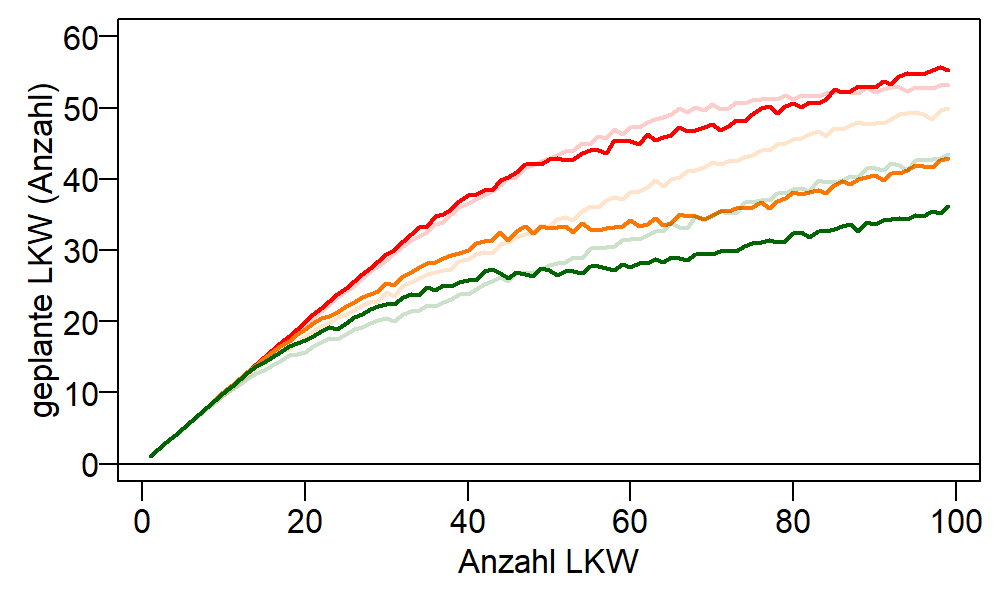
\includegraphics[width=\linewidth]{images/graphs/rsCategoryDistributionSjn.png}
  \caption{Shortest Job Next}
  \label{fig:ecd1}
\end{subfigure}
\begin{subfigure}{.495\textwidth}
  \centering
  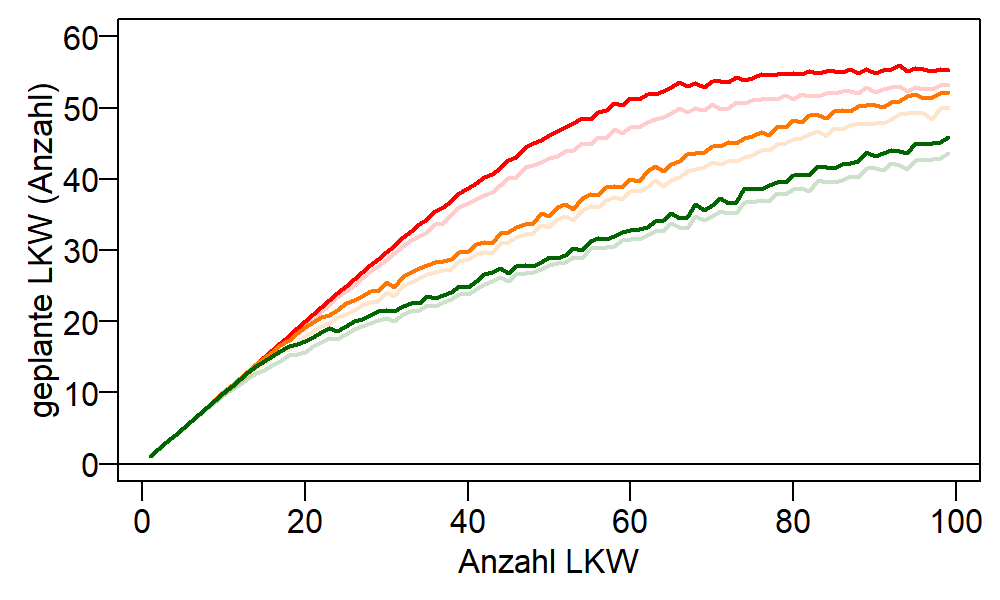
\includegraphics[width=\linewidth]{images/graphs/rsCategoryDistributionMit.png}
  \caption{Most Idle Time}
  \label{fig:ecd2}
\end{subfigure}

\begin{subfigure}{.5\textwidth}
  \centering
  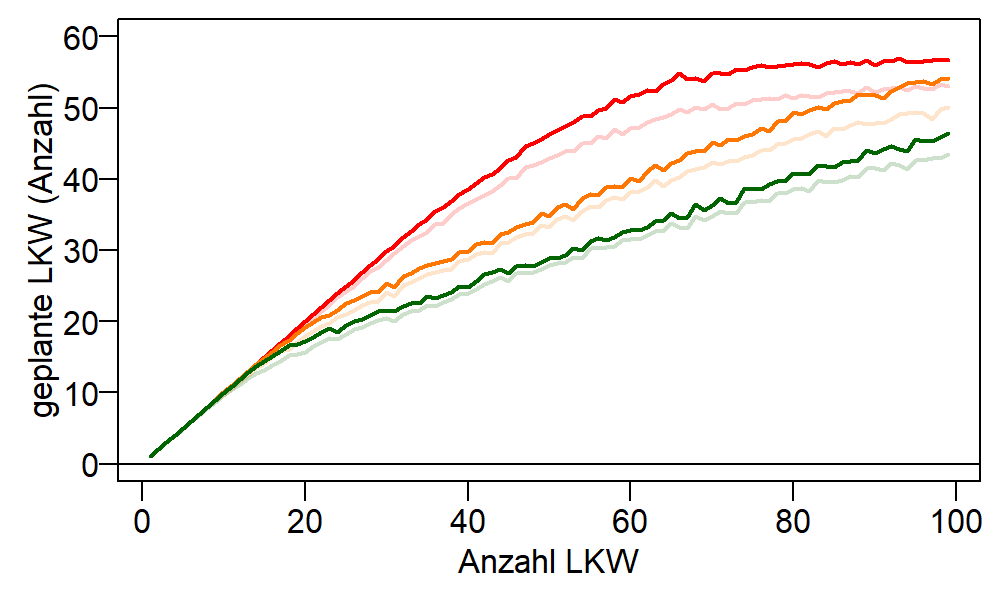
\includegraphics[width=\linewidth]{images/graphs/rsCategoryDistributionFcfs.png}
  \caption{First come, first served}
  \label{fig:ecd3}
\end{subfigure}
\caption{Geplante LKW bei steigender Ungleichverteilung der Abfertigungskategorien}
\label{fig:evalCategoryDist}
\end{figure}
\todo{Legende}

Auch dieses letzte Testszenario verfestigt das Bild und die Bewertung, welche schon zuvor über die einzelnen Verfahren gewonnen wurde. 

Das SJN Verfahren (siehe Graph \ref{fig:ecd1}) zeigt wie auch schon zuvor festgestellt wenig Verbesserung und sogar eine teilweise Verschlechterung der Anzahl der abgefertigten LKW. Extremer wird dieses Verhalten sogar, bei der hier gezeigten Ungleichverteilung. Gegenüber der ausgeglichenen Verteilung ergibt sich hier zunächst ein starker negativer Sprung, aber auch gegenüber der jeweils unoptimierten Kurve sind hier starke Verschlechterungen erkennbar. Je ungleicher die Verteilung wird, das Ergebnis aber nicht mehr ganz so viel schlechter. Es ist allerdings auch zu erkennen, dass die Verbesserung gegenüber dem unoptimierten Fall im unteren Bereich zwischen etwa 20 und 40 LKW leicht steigt, wenn die Verteilung unausgeglichener ist. Insgesamt war dieses Verfahren aber ohnehin schon kein Favorit für einen realen Einsatz, spätestens aber wenn keine gute Prognose der Verteilung der ankommenden LKW möglich ist und somit keine dazu passenden Ressourcen zur Verfügung gestellt werden können, verschlechtert sich die Performance stark.

Die Verfahren MIT und FCFS, verhalten sich hier wie auch schon in den vorherigen Auswertungen sehr ähnlich, wie Graphen \ref{fig:ecd1} und \ref{fig:ecd2} zeigen. Auch hier hat FCFS mit höherer Zahl von LKW wieder leicht höhere Werte als MIT. Erkennbar ist, dass die Anzahl der erfolgreich eingeplanten LKW deutlich sinkt, wenn es eine stärkere Ungleichverteilung gibt. Gleichzeitig nimmt auch die Verbesserung gegenüber dem unoptimerten Fall ab. Im für einen 180 Minuten Slot interessanten Fall bis ca. 60 LKW erreicht der Unterschied der Kurven sein Maximum. Dass sich der Nachteil dieser Verteilung mit noch weiter steigender Zahl wieder verringert, ist also in der Realität weniger relevant. Es lässt sich daraus schließen, wie auch schon zu erwarten war, dass es schon im vorhinein das Ziel sein sollte, eine möglichst gute Prognose der ankommenden LKW zu haben, zumindest was die Verteilung der Ladungstypen angeht. Wenn einfach keine passenden Aufträge für die zur Verfügung stehenden Maschinen hereinkommen, kann auch der beste Algorithmus keine gute Auslastung aller Ressourcen erzeugen. Dennoch erkennt man, dass beide Algorithmen weiterhin eine verbesserte Verteilung und somit die Planung von mehr LKW ermöglichen, auch wenn dieser Vorteil natürlich geringer wird.


\subsection{Auswertung Algorithmus 2 (TSP)}

Die Kernpunkte der Auswertung des zweiten Algorithmus unterscheiden sich etwas von den Zielen der anderen Auswertung. Zum einen soll hier auch wieder eine Bewertung hinsichtlich der Art und Höhe der möglichen Optimierungen stattfinden. Im Unterschied zur anderen Umsetzung sollen die Lösungsverfahren des TSP theoretisch die gleiche, beste Lösung ermitteln. Ein erstes Ziel wäre es also alle Verfahren bezüglich ihrer Nutzbarkeit und Praxisuntauglichkeit zu bewerten, um alle anschließenden Tests dann nur mit dem daraus bestimmten, besten Verfahren durchzuführen.

\subsubsection{Testszenario 1: Bestimmung der Parameter für das Simulated Annealing Verfahren}

Bevor die Verfahren gegeneinander bewertet werden können, müssen zunächst einmal die besten Werte für das Simulated Annealing Verfahren gefunden werden. Die variablen Paramater sind dabei: startingTemperature, coolingRate und numberOfIterations. Ziel dieses Testszenarions ist es, diese Parameter zu variieren und so die bestmöglichen Eingabewerte für den gegebenen Anwendungsfall zu finden. In der Testklasse \textit{SimAParameterTest} wurden dafür die im Folgenden beschriebenen Abläufe implementiert, mit dem R-Skript \textit{tspSimAParameter} wurden die Ergebnisse ausgewertet, sowie die hier dargestellten Graphen erzeugt.

Schaut man sich die Implementierung des Algorithmus genauer an, so ist numberOfIterations einfach die maximale Anzahl von Schleifendurchläufen und sozusagen eine Begrenzung, damit der Algorithmus im schlimmsten Fall nicht ewig läuft. Um diesen Parameter sinnvoll einschätzen zu können, wurden alle folgenden Testdurchläufe mit dem Wert Integer.MAX\_VALUE durchgeführt, somit wird es so viele Schleifendurchläufe geben, wie es braucht. Die benötigte Anzahl wird hier jeweils in die CSV-Datei mit den Ergebnisdatensätzen übernommen. Somit können hier im Nachhinein die höchsten benötigten Werte abgelesen werden, um eine sinnvolle Einschätzung der notwendigen Iterationen zu erhalten und für den Worst-Case ein mit Spielraum versehenes Limit gesetzt werden. Hauptsächlich abhängig ist das Ergebnis des Algorithmus also von startingTemperature und coolingRate. Die startingTemperature darf sich dabei in einem theoretischen Bereich von >0,1 und unendlich bewegen. Die coolingRate muss für sinnvolle Ergebnisse >0 und <1 sein. Um hier einen Gesamteindruck der Auswirkung dieser beiden Parameter auf das Ergebnis zu erhalten, sollen diese beiden Variablen systematisch in Schleifen variiert werden und jeweils die Kosten berechnet werden. Es entsteht somit ein dreidimensionaler Datensatz der Kosten in Abhängigkeit von startingTemperature und coolingRate. Für das Gesamtbild wird ein zufälliger, aber fester Graph generiert. Mit diesem wird der SimA Algorithmus mit jeder Kombination von startingTemperature und coolingRate einmal ausgeführt. Um das Verhalten über verschiedenen Graphen zeigen zu können, wird dieser gesamte Prozess mit 100 verschiedenen Graphen ausgeführt. In ersten, losen Test hat sich gezeigt, dass der wirklich interessante Teil bei startingTemperature etwa im Intervall [1;100] liegt und die coolingRate etwa bei [0.9;1[. Um die Übersichtlichkeit zu wahren und die Ausführungsdauer der Tests einzuschränken, wurden die Tests deshalb auf diese Intervalle konzentriert. Die startingTemperature wurde dabei in Schritten von 1 erhöht, die coolingRate jeweils um 0,001.

Nachfolgende Graphen (Abb. \ref{fig:evalSimAParams}) zeigen das Ergebnis dieser Auswertung. Gezeigt werden dabei in einem farblichen Verlauf die durchschnittlichen Kosten über aus den 100 Durchläufen mit verschiedenen Graphen zu einem Paar aus startingTemperature und coolingRate. Die grünen Bereiche zeigen dabei, wo die Kosten tendenziell am geringsten sind und die roten Bereiche repräsentieren die höchsten Kosten. Da auch die Größe des zu bearbeitenden Graphen einen Einfluss hat, wurde dieser gesamte Test mit Graphen mit den Größen 10, 20, 50 und 100 Knoten wiederholt. Mit Blick auf die zu erwartenden LKW \todo{in konzeption/Anforderungen erwähnen?!} wird dies wird voraussichtlich der Bereich sein, in dem der Algorithmus zum Lösen des TSP verwendet wird.

\begin{figure}[H]
\centering
\begin{subfigure}{.495\textwidth}
  \centering
  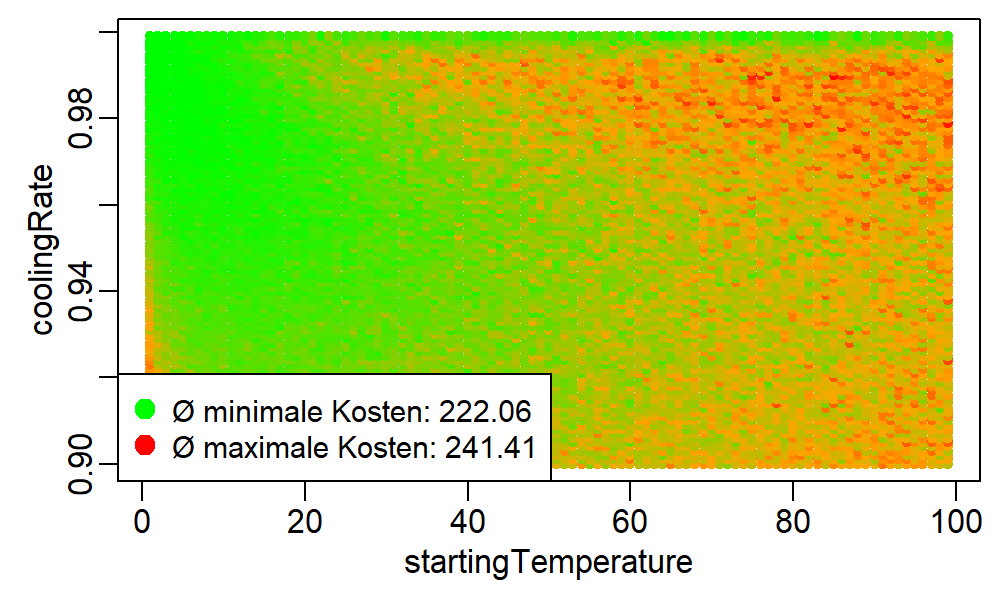
\includegraphics[width=\linewidth]{images/graphs/tspSimAParameter10.png}
  \caption{Graph mit 10 Knoten}
  \label{fig:esp1}
\end{subfigure}
\begin{subfigure}{.495\textwidth}
  \centering
  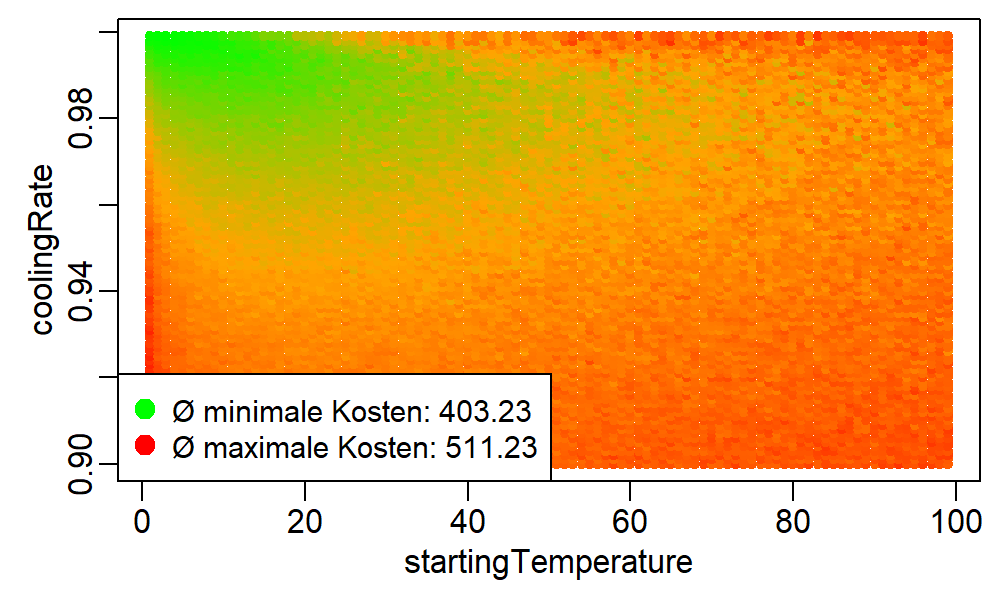
\includegraphics[width=\linewidth]{images/graphs/tspSimAParameter20.png}
  \caption{Graph mit 20 Knoten}
  \label{fig:esp2}
\end{subfigure}

\begin{subfigure}{.495\textwidth}
  \centering
  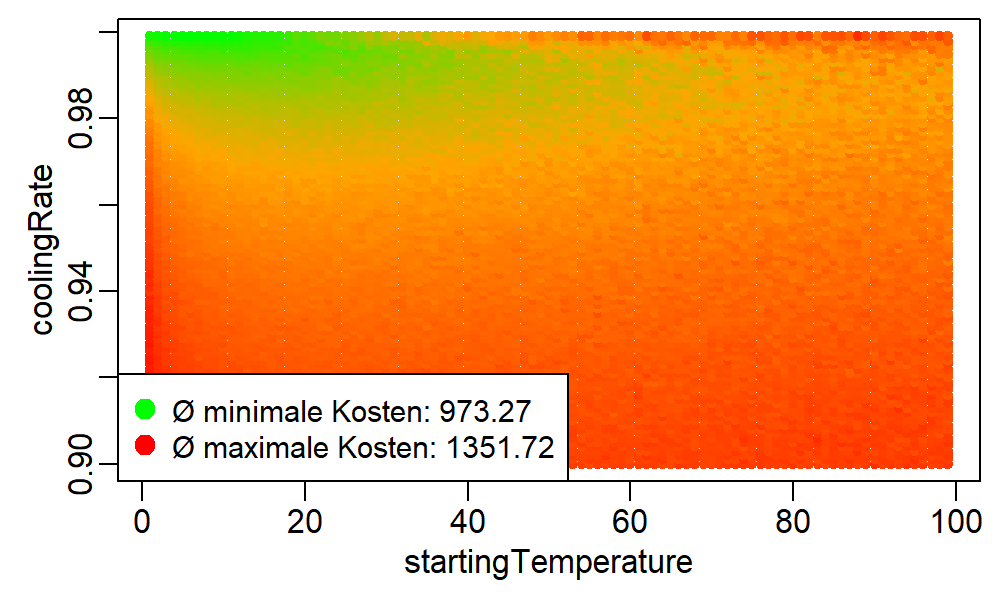
\includegraphics[width=\linewidth]{images/graphs/tspSimAParameter50.png}
  \caption{Graph mit 50 Knoten}
  \label{fig:esp3}
\end{subfigure}
\begin{subfigure}{.495\textwidth}
  \centering
  \includegraphics[width=\linewidth]{images/graphs/tspSimAParameter100.png}
  \caption{Graph mit 100 Knoten}
  \label{fig:esp4}
\end{subfigure}
\caption{Simualted Annealing mit variierten Parametern}
\label{fig:evalSimAParams}
\end{figure}

Für die besten Werte der Parameter lassen sich daraus nun einige Schlussfolgerungen ziehen. Zur benötigten Anzahl von Iterationen lässt sich aus den resultierenden Wertetabellen ablesen, dass diese relativ stark schwankt, das Maximum liegt in diesem Beispiel aber bei 6895\todo{finalen Wert eintragen}. Selbst wenn man die Grenze für den Worst-Case nun extrem großzügig auf beispielsweise 100.000 setzt, ist dies immer noch ein Wert, der in der Berechnung problemlos handhabbar ist. Selbst diese Zahl von Iterationen sollte nicht für nennenswert hohe Ausführungszeiten sorgen. Diese Höhe von Iterationen wird aber wenn überhaupt ohnehin extrem selten erreicht.

Die dargestellten Graphen lassen nun eine gute Einschätzung zu, wie die beiden weiteren Parameter zu wählen sind. Grundsätzlich werden sich dabei keine exakten Werte bestimmen lassen, da es sich hier immer noch um Zufallswerte handelt, für die immer etwas andere Parameter optimal wären. Gerade bei geringer Anzahl von Knoten ist zu erkennen, dass die Kosten auch bei nah aneinander liegenden Punkten deutliche Schwankungen haben, da sehr unterschiedlich farbige Punkte nah beieinander liegen und kein gleichmäßiger Verlauf entsteht. Dennoch lässt sich eine sehr gute Tendenz erkennen, bei welcher Kombination von Parametern die Kosten optimal gering werden. Bei geringer Anzahl von Knoten ist die Wahl der Parameter noch nicht ganz so kritisch, hier ist der optimale, grüne Bereich noch relativ groß. Hier würde eine startingTemperature $<$ 50 und eine coolingRate $>$ 0,9 in der Regel schon sehr gute Werte liefern. Mit größerer Anzahl von Knoten wird dieser Bereich deutlich kleiner. Hier sollte vor allem die coolingRate so nah wie möglich an 1 liegen. Gute Werte werden hier tendenziell nur noch bei startingTemperature $<$ 40 und coolingRate $>$ 0,99 erzielt. Die grünen Bereiche der Graphen überschneiden sich allerdings, was sehr gut es, denn gut Werte für 100 Knoten liefern somit auch z.B. bei 10 Knoten ebenfalls gute Ergebnisse. Eine startingTemperature von 15 und eine coolingRate von 0,9995 sollten also gut geeignet sein.

Abschließend wurden die hier ermittelten Werte (numberOfIterations=100.000, startingTemperature=15, coolingRate=0,9995) als Standardwerte in die Variablen der Klasse \textit{SimulatedAnnealingAlgorithm} übernommen. Über in diesen Tests verwendeten Konstruktor können wie bisher variable Werte verwendet werden, werden diese Werte allerdings über den weiteren Konstruktor nicht gesetzt, so werden immer die hier ermittelten, besten Werte verwendet. Alle weiteren Testszenarien arbeiten also dann direkt mit diesen Werten.

\subsubsection{Testszenario 2: Laufzeit und Grenzen}
\todo{Leistungsdaten des Rechners angeben?!}

Wie schon bei der Implementierung aufgefallen ist, werden insbesondere die exakten Verfahren früher oder später durch ihre Laufzeit bei der Berechnung oder durch ihren Arbeitsspeicherbedarf begrenzt sein. Der nötige Aufwand ist dabei zum bedeutendsten Teil von der Anzahl der Knoten des zu lösenden Graphen abhängig. Um also zunächst die Lösungsverfahren selbst zu bewerten, sind hier noch gar keine Vergleiche und Auswertungen hinsichtlich des eigentlichen Problemszenarios nötig. Viel mehr ist hier die Laufzeit bei der Berechnung der Ergebnisse für die einzelnen Verfahren von Interesse. Aus diesem Grund arbeiten die folgenden Tests, welche in der Testklasse \textit{RunTimeTest} implementiert wurden auch direkt mit den Algorithmus-Klassen, ohne Ladeplätze, Slotlimiterungen o.ä. zu berücksichtigen. Ausgeführt wird also immer jeder Algorithmus einmal mit dem identischen Eingangsgraphen. Dabei wird schrittweise die Anzahl der Knoten erhöht. Für jede Anzahl von Knoten werden dabei 10 Durchläufe mit unterschiedlichen, zufälligen Graphen erzeugt, um sinnvolle Durchschnittswerte und Streuungen bei der Berechnungszeit ermitteln zu können. Da hier keine exakten Ergebnisse, sondern vor allem Größenordnungen interessant sind, reichen hier 10 Wiederholungen. Um die Ausführungszeit darüber hinaus im Rahmen zu halten, wurde ein Begrenzung eingebaut, sodass die Algorithmen für mehr Knoten nicht mehr ausgeführt werden, wenn entweder einmal der Speicherplatz ausgegangen ist oder wenn die Ausführung zu lange gedauert (Limit von 10 Minuten) \todo{Erhöhen für eine Ausführung von 16 Knoten?!} hat. Die Tendenz sollte dann erkennbar sein und eine stunden- oder tagelange Ausführung der Tests ist nicht nötig. Die folgende Auswertung (Tabelle \ref{tab:evalTspRunTime}) wurde durch das R-Skript \textit{tspRunTime.R} berechnet. Als Darstellungsform wurde in diesem Fall eine Tabelle gewählt, da sich die Werte stark voneinander unterscheiden. Die wichtigen Aspekte wären in einem Graphen nicht gut sichtbar.


\begin{table}[H]
    \caption{Durchschnittliche Laufzeiten der Verfahren (Alle Werte in s)}
    \label{tab:evalTspRunTime}
    \centering
    \begin{tabular}{c|c|c|c|c|c|c}
        \textbf{Knoten} & \textbf{Ø SimA} & \textbf{$\sigma$ SimA} & \textbf{Ø BnB} & \textbf{$\sigma$ BnB} & \textbf{Ø RM} & \textbf{$\sigma$ RM} \\\hline\hline
        \csvreader[
            %column count=4,
            %no head,
            %table head=\hline\hline,
            %table head=\textbf{Labels} & \textbf{Labels} & \textbf{Labels} & \textbf{Labels} \\\hline,
            late after line=\\\hline,
            late after last line=\\
        ]
        {files/tspRunTime_out.csv}
        {1=\one, 2=\two, 3=\three, 4=\four, 5=\five, 6=\six, 7=\seven, 8=\eight}
        {\two & \three & \four & \five & \six & \seven & \eight}
    \end{tabular}
\end{table}
\todo{Mit mehr Durchläufen asuführen, sternchen an einfach ausgeführten einfügen}

Sehr deutlich zu erkennen ist, dass der Aufwand zum Lösen des Problems exponentiell mit der Anzahl der Knoten steigt. Insbesondere für das Reduced Matrix und das Branch and Bound Verfahren bedeutet dies, dass der Aufwand ab etwa 10 Knoten merklich höher wird und jeweils bei 13 bzw. 15 Knoten so groß wird, dass dies zumindest für eine größere Zahl von Wiederholungen in dieser Auswertung deutlich zu viel ist. Das Reduced Matrix Verfahren scheitert dabei an einem \glqq{}java.lang.OutOfMemoryError: Java heap space\grqq{} Fehler, welcher zeigt, dass der Arbeitsspeicher der Java VM nicht ausreicht, selbst mit einer Erhöhung auf 8 GB. Die Laufzeit der Berechnung steigt zwar auch erheblich, aber dem ersten Anschein nach nicht so schnell wie im Branch and Bound Verfahren. Hier kostet bereits die Berechnung von 15 Knoten im Durchschnitt ca. 16 Minuten, während es bei 14 Knoten noch ca. 3 Minuten waren. Aus diesem Grund wurden auch die letzten Durchläufe jeweils nur mit einer Wiederholung durchgeführt und bilden somit nur einen Anhaltspunkt der Ausführungszeit, aber keinen sinnvollen Durchschnitt mehr\todo{finaler Stand?}. Bei diesen Verfahren zeigt sich aber auch eine hohe Standardabweichung bei der Ausführungszeit zwischen verschiedenen Durchläufen. Dies dürfte damit zusammenhängen, dass diese Verfahren je nach Eingabewerten unterschiedlich viel Zeit sparen. Das Simulated Annealing Verfahren zeigt dagegen über wesentlich längere Zeit deutlich geringere Ausführungszeiten. Insgesamt ist bei der mehrfachen Ausführung dieser Testklasse sichtbar geworden, dass die Ausführungszeiten auch zwischen diesen Ausführungen schwanken. Dies hat insbesondere beim Branch and Bound Verfahren mit 14 Knoten einen sichtbaren unterschied von einigen Sekunden gemacht. Dies dürfte auch mit der sonstigen Auslastung des Computers im Hintergrund zu tun haben. Eine deutliche Tendenz ist aber sehr klar sichtbar und ändert nichts an den extrem steigenden Zeiten.




\textbf{Qualität der Verfahren}

Gleichzeitig sind die Werte dieses Szenarios ein guter Anhaltspunkt, um die Qualität der Verfahren untereinander zu vergleichen. Insbesondere das Simulated Annealing Verfahren findet nicht unbedingt das beste Ergebnis, sodass hier auch gleichzeitig ein direkter Vergleich stattfinden kann. Als Metrik bietet sich hier die Höhe der Gesamtkosten bzw. der Gesamtzeit des gefundenen Weges durch den Graphen an, da dies auch der Wert ist, nachdem beim TSP optimiert wird. Diese zweite Auswertung (siehe Tabelle \ref{tab:evalTspTotalCost}) wurde mit den identischen CSV-Daten durch das R-Skript \textit{tspTotalCost.R} berechnet. Auch hier wurde die Darstellung in einer Tabelle gewählt, da übereinanderliegende und starkt steigende Werte so deutlich besser sichtbar sind.

\begin{table}[H]
    \caption{Durchschnittliche Kosten der Verfahren (Alle Werte in min)}
    \label{tab:evalTspTotalCost}
    \centering
    \begin{tabular}{c|c|c|c|c|c|c}
        \textbf{Knoten} & \textbf{Ø SimA} & \textbf{$\sigma$ SimA} & \textbf{Ø BnB} & \textbf{$\sigma$ BnB} & \textbf{Ø RM} & \textbf{$\sigma$ RM} \\\hline\hline
        \csvreader[
            late after line=\\\hline,
            late after last line=\\
        ]
        {files/tspRunTime_costOut.csv}
        {1=\one, 2=\two, 3=\three, 4=\four, 5=\five, 6=\six, 7=\seven, 8=\eight}
        {\two & \three & \four & \five & \six & \seven & \eight}
    \end{tabular}
\end{table}
\todo{Mit mehr Durchläufen ausführen, sternchen an einfach ausgeführten einfügen}

\todo{Streuung sinnvoll, da immer andere Graphen?! Oder hier evtl Variationskoeffizient, um relative schwankung darzustellen?}

Erkennbar ist, die exakten Verfahren BnB und RM durchgängig identische Werte liefern. Die Abweichung von RM bei 13 Knoten ist damit zu erklären, dass hier aufgrund vom Speichermangel nicht mehr alle Durchläufe berechnet werden konnten, während es bei BnB ein Durchschnitt aus allen 10 Iterationen ist. Auch das SimA Verfahren zeigt bis 10 Knoten identische Werte. Dies zeigt, dass in diesen Bereichen von allen Verfahren das gleiche und serh wahrscheinlich auch optimale Ergebnis erzielt wurde. Ab 11 Knoten fängt es an, dass die Ergebnisse des SimA Verfahrens etwas schlechter werden, als die höchst wahrscheinlich optimalen Ergebnisse der anderen Verfahren. Aufgrund der bereits erkannten Beschränkungen bezüglich Laufzeit und Speicherbedarf lässt sich diese Tendenz so einfach nicht weiter bestätigen. Dies bestätigt aber auch die Theorie des Simulated Annealing, dass eben in der Regel ein sehr gutes, aber nicht perfektes Ergebnis erzielt wird \todo{Quelle?}. Somit lässt sich vermuten, dass die Ergebnisse auch bei einer sehr viel größeren Zahl von Knoten sehr gut sind.

Insgesamt zeigt sich als großer Vorteil des Simulated Annealing Verfahrens, dass schon mit einfachen Rechen-Ressourcen eine wesentlich höhere Zahl von Knoten, weit über 1000 Knoten möglich ist. Dies übersteigt die hier realistisch zu erwartende Größe von Graphen um ein vielfaches. Insbesondere wenn ein mTSP, also eine Verteilung für mehrere Ladeplätze ermittelt werden soll und somit noch einige Knoten für Ladeplätze verbraucht werden, sind 12-15 Knoten sehr schnell erreicht. Ein sinnvoller Einsatz von Branch and Bound und Reduced Matrix Verfahren ist (in der hier implementierten Variante) also eigentlich nicht möglich. Selbst wenn man die Rechen-Ressourcen deutlich aufstockt, wird der Bedarf weiter exponentiell steigen. Damit ist möglicherweise eine Erhöhung der Knotenanzahl im unteren einstelligen Bereich möglich, eine sinnvoll nutzbare Anzahl wird dies aber höchstwahrscheinlich immer noch nicht. Für die weiteren Tests wird deshalb mit dem Simulated Annealing Verfahren weiter gearbeitet.


\subsubsection{Testszenario 3: Streuung zwischen den Simulated Annealing Durchläufen}

In diesem Szenario geht es darum, wie groß die Streuung der optimierten Kosten beim mehreren Durchläufen des selben Graphen ist. Während vorherigem explorativen Ausprobierens der Verfahren ist aufgefallen, dass sich die Ergebnisse, also die Gesamtkosten zwischen den Durchläufen eines eigentlich identischen Graphen unterscheiden. Dies dürfte aber nur für den Simulated Annealing Ansatz relevant sein, da hier mit gewissen Zufallsprozessen, dem \glqq{}Abkühlungsvorgang\grqq{} gearbeitet wird. Bei den anderen Verfahren ergibt sich immer das beste Ergebnis, bei allerdings höherer Rechenzeit, wie die vorherigen Tests gezeigt haben. Da mit dem Simulated Annealing Verfahren weiter gearbeitet werden soll, soll dieser Umstand an dieser Stelle aber noch einmal genauer untersucht werden.

Das Vorgehen, welches in der Testmethode \textit{spreadTest()} der Testklasse \textit{SimulatedAnnealingTest} implementiert wurde und zur Ermittlung passender Werte dient, ist wie folgt: Die prinzipielle Idee ist es, das Simulated Annealing Verfahren mit dem identischen Eingangsgraphen mehrfach laufen zu lassen. Es wird dabei bei jeden weiteren Durchlauf immer das beste Ergebnis, also die geringsten Durchlaufkosten aller vorherigen Iterationen gespeichert. Die Idee dabei ist, dass man angesichts des geringen Zeitaufwands eines SimA Durchlaufs einfach immer mehrere Durchläufe macht und das insgesamt beste Ergebnis zurück gibt. Um auch hier wieder einen aussagekräftigen Durchschnitt ermitteln zu können, wird das Ganze in einer Schleife mit 100 verschiedenen Graphen durchgeführt. Dargestellt wird immer die prozentuale Abweichung von dem insgesamt für diesen Graphen besten ermittelten Wert, welcher nach Formel \ref{eq:simaResBestCost} berechnet wurde. Diese Darstellung wurde gewählt, da der absolut beste Wert je nach Graphen etwas unterschiedlich ist. In dieser Aufbereitung lässt sich ein besserer Vergleich ziehen. Allerdings ist dieser Wert auch nicht als überhaupt minimal erreichbarer Wert zu verstehen, aber auch bei noch wesentlich mehr Durchläufen bleibt die Kurve nicht konstant bei 0\%, da es sich aber um wenige Fälle und nur noch minimale Verbesserungen handelt, wurde hier der Übersicht halber 70 Durchläufe als Maximum gewählt. Als Größe für den Graphen wurden hier exemplarisch 50 LKW bei 3 Ladeplätzen gewählt, was mit insgesamt 53 Knoten im oberen erwartbaren Bereich liegt, was die potenzielle Größe der Graphen angeht. Je Größer der Graph ist, desto mehr Algorithmus Durchläufe wird es tendenziell benötigen, um das absolut mögliche Minimum zu finden.

\begin{equation} \label{eq:simaResBestCost}
relativ Beste Kosten = \left(\left(\frac{absolut Beste Kosten}{minimale Kosten Der Iteration}\right)*100\right)-100
\end{equation}

\begin{figure}[H]
    \centering
    \includegraphics[width=0.7\textwidth]{images/graphs/tspResultSpreadTest.png}
    \caption{Bestes Ergebnis des Simualted Annealing Verfahrens nach mehreren Durchläufen}
    \label{fig:tspEvalSpread}
\end{figure}

\todo{Legende}

In Abbildung \ref{fig:tspEvalSpread} ist erkennbar, dass es zu Beginn mit nur einem einzigen Algorithmuslauf eine sehr große Unsicherheit gibt. Im Durchschnitt ist das Ergebnis etwa 12\% schlechter, als es im besten Fall nach 70 Durchläufen möglich war. Auch die Standardabweichung ist extrem hoch, d.h. es gibt Fälle in denen das Ergebnis nach einem Durchlauf bereits sehr gut ist, in anderen Fällen ist dies da aber noch sehr viel schlechter. Die Kurve sinkt allerdings schon nach wenigen Durchläufen sehr stark. Nach etwa 5 Läufen ist das Ergebnis im Mittel nur noch ca. 3\% schlechter bei auch sehr viel geringerer Streuung. Ab ca. 10 Läufen werden die Ergebnisse auch deutlich langsamer besser.  Für den realen Einsatz des Simulated Annealing Verfahrens lässt sich daraus schlussfolgern, dass eine wiederholte Ausführung zum finden des besten Ergebnisses durchaus sinnvoll ist. Schon eine 5 bis 10-fache Iteration kann die größten Unsicherheiten beseitigen. Angesichts der wirklich sehr geringen Laufzeiten im Millisekunden-Bereich (siehe Tabelle \ref{tab:evalTspRunTime}), kann man sogar über eine wesentlich höhere Zahl von 30 bis 50 oder sogar noch mehr Durchläufen nachdenken. Selbst wenn dann Berechnungszeiten von wenigen Sekunden entstehen, ist dass für den realen Einsatz noch lange kein Problem.


\subsubsection{Testszenario 4: Verbesserung der Abfertigungszeit}

Nachdem nun viel Aufwand in die Bestimmung des besten Lösungsverfahrens sowie in die beste Verwendung der Verfahren geflossen ist, sollen nun Versuche zum eigentlichen Ziel der Optimierung durchgeführt werden. Gearbeitet werden soll dabei, wie in den vorherigen Tests bestimmt wurde, mit dem Simulated Annealing Alogrithmus. Genutzt wird immer das beste Ergebnis aus 50 Durchläufen. Außerdem werden die Buchungen immer auf 3 Ladeplätze aufgeteilt. Interessant ist hier in erster Linie, wie viel sich die gesamte Abfertigungszeit gegenüber dem unoptimierten Ausgangszustand verbessern lässt. Es wird dabei immer die durch den SimA-Algorithmus optimierten Wert mit den unoptimierten Werten verglichen, welche mit aus der Zeitplanung des UnoptimizedAlgorithm ermittelt wurden. Einmal soll das Ganze für einen unbegrenzten Zeitraum simuliert werden. Die gleichen Tests werden aber auch noch einmal für einen begrenzten Slot durchgeführt werden. Interessant sind diese Werte, da dies auch schlussendlich das für den realen Einsatz bedeutende Ergebnis ist. Da die Begrenzung allerdings ein weiterer, auf die eigentliche Optimierung aufbauender Schritt ist, wird hier diese getrennte Betrachtung durchgeführt. Implementiert wurden die Tests in den Testmethoden \textit{test3LoadersBestOf50()} und \textit{test3LoadersBestOf50Limited()} der Testklasse \textit{SimulatedAnnealingTest}. Das R-Skript \textit{tspOptimization.R} diente zur Auswertung.

Im Graphen dargestellt ist zum einen, wie sich die Gesamtzeit verbessert hat, bis alle LKW bearbeitet wurden. Berechnet wurde dieser Wert nach Formel \ref{eq:tspCostSaving}. Zusätzlich ist eine Kurve sichtbar, welche die Verbesserung bei der Zahl der eingeplanten LKW zeigt. Dieser Wert wird über Formel \ref{eq:tspSchedImpr} berechnet. Beide Werte werden prozentual dargestellt, da so ein relativer Vergleich mit steigender Anzahl von LKW Buchungen möglich ist.

\begin{equation} \label{eq:tspSchedImpr}
schedImpr = \dfrac{oScheduledJobs-uScheduledJobs}{uScheduledJobs} * 100
\end{equation}

\begin{equation} \label{eq:tspCostSaving}
costImpr = \dfrac{uCost-oCost}{uCost} * 100
\end{equation}

%\begin{equation} \label{eq:tspTtcSaving}
%ttcSaving = \dfrac{uTimeToComplete-oTimeToComplete}{uTimeToComplete} * 100
%\end{equation}


\begin{figure}[H]
\centering
\begin{subfigure}{.495\textwidth}
  \centering
  \includegraphics[width=\linewidth]{images/graphs/tspSimulatedAnnealingUnlimited.png}
  \caption{Unbegrenzter Slot}
  \label{fig:etspsimaopt2}
\end{subfigure}
\begin{subfigure}{.495\textwidth}
  \centering
  \includegraphics[width=\linewidth]{images/graphs/tspSimulatedAnnealingLimited.png}
  \caption{3 Stunden Slot}
  \label{fig:etspsimaopt2}
\end{subfigure}
\caption{Verbesserung der Abfertigungszeit}
\label{fig:evalTspSimAOpt}
\end{figure}

\todo{Time to complete darstellen?; Punkte weg, nur linie}

Zunächst einmal ist an den Ergebnisgraphen zu erkennen, dass mit dem hier untersuchten Algorithmus definitiv gute Verbesserungen erzielt werden können. Gibt es keine Slotbegrenzung, so können immer alle LKW abgefertigt werden, die rote Linie ist also konstant bei 0, da die Zahl der geplanten LKW in beiden Modellen identisch ist. Die Gesamtzeit, die es braucht, alle LKW zu bearbeiten verbessert sich dagegen. Zunächst einmal steigt diese Verbesserung stark an, sodass bereits bei 10 LKW eine über 20\% kürzere Abfertigungszeit möglich ist. Dann steigt die Verbesserung immer langsamer und nähert sich bis ca. 50 LKW den 40\% an. Die Standardabweichung, also die Streuung der Gesamtabfertigungszeit ist über den gsamten Bereich nicht besonders hoch, verringert sich aber mit streigender Anzahl von LKW noch einmal. Viel interessanter ist allerdings das Verhalten bei begrenztem Slot. Bis ca. 14-15 LKW verhalten sich beide Kurven sehr ähnlich, hier entstehen durch die Slotbegrenzung noch gar keine Einflüsse, im unoptimierten, wie im optimierten Fall können hier noch alle LKW eingeplant werden. Die Verbesserung der Abfertigungszeit erreicht hier auch sein Maximum. Ab dann verbessert sich die Zahl der LKW, welche eingeplant werden können. Im unoptimierten Fall müssen nun langsam die ersten LKW abgewiesen bzw. in andere Slots verschoben werden. Die Zahl der eingeplanten LKW steigt nun sehr stark an und erreicht bei 50 gebuchten LKW knapp 60\% Verbesserung. Allerdings erhöht sich auch die Streuung extrem, d.h. es gibt Fälle in denen deutlich mehr LKW erfolgreich eingeplant werden können, als in anderen. Die Verbesserung der gesamten Abfertigungszeit sinkt ab ca. 15 LKW wieder und nähert sich bei gleichbleibender Streuung der 0 an. Dies liegt daran, dass der Slot in beiden Fällen sehr gut voll ausgelastet wird. Allerdings ist die Zeit pro LKW deutlich geringer, sodass mehr LKW in die gleiche Zeit passen, wie die andere Kurve eben gezeigt hat. 

Insgesamt lässt sich aus diesem Test schlussfolgern, dass mit dem hier getesteten Verfahren durchaus gute Verbesserungen erzielt werden können. Die Höhe der Verbesserung hängt davon ab, wie viele LKW pro Slot gebucht werden dürfen, bzw. ob und in welcher Höhe Überbuchungen erlaubt werden. So hat der Algorithmus mehr Planungsspielraum, es müssten allerdings auch Buchungen auf andere Slots verschoben werden. Um hie die optimale Größe zu finden, wurde das nächste Testszenario durchgeführt.

\subsubsection{Testszenario 5: Verhalten bei Überbuchung}

Wie im vorherigen Szenario festgestellt wurde, hat die Zahl der LKW, welche einen Slot buchen können einen bedeutenden Einfluss auf die Höhe der möglichen Verbesserung. Es stellt sich nun die Frage, ob man eine harte Grenze einführen sollte und keine Buchungen mehr zulässt, wenn die erste Buchung nicht mehr in den Slot passt. Die andere Option wäre es, wie es auch schon für den anderen hier entwickelten Algorithmus empfohlen wurde, eine gewissen Überbuchung zuzulassen. In diesem Fall müssten einige Buchungen zwangsweise im Nachhinein auf spätere Slots verschoben werden. So ergibt sich aber ein noch größerer Spielraum für den Planungsalgorithmus und somit möglicherweise noch weiter verbesserte Abfertigungszeiten. 

Ein entsprechender Testfall wurde in der Testklasse \textit{SimulatedAnnealingTest} in der Methode \textit{test3LoadersBestOf50LimitedOverfill()} implementiert. Der Grundaufbau und die gesammelten Daten sind dabei wie im vorherigen Test. Hier wird allerdings für ein Testreihe die gleiche Liste von Buchungen beibehalten und nur schrittweise eine weitere hinzugefügt. Dies simuliert, dass weitere LKW Fahrer bzw. Speditionen diesen Slot buchen. Dargestellt wird im Auswertungsgraphen dieses mal aber die absolute Zahl von Buchungen, um zeigen zu können, wann nicht mehr alle LKW eingeplant werden können. Eine diagonale Gerade der Steigung 1 zeigt dann des theoretischen Anstieg, ohne begrenzten Slot. Auf einer zweiten y-Achse wird dagegen die Verbesserung der Gesamtkosten aufgetragen, berechnet nach dem gleichen Weg, wie im vorherigen Szenario (siehe Formel \ref{eq:tspCostSaving}).

\begin{figure}[H]
    \centering
    \includegraphics[width=0.7\textwidth]{images/graphs/tspSimALimOverfill.png}
    \caption{Verhalten bei Überbuchung}
    \label{fig:tspEvalOverfill}
\end{figure}

In der Auswertung ist gut zu erkennen, dass selbst bei strikter Begrenzung des Slots eine deutliche Verbesserung möglich ist. Während die blaue Kurve schon bei etwa 14 LKW abfällt und somit zeigt, dass schon nicht immer alle LKW in den Slot passen, fängt die rote, optimierte Kurve erst bei etwa 22 LKW an, langsam abzufallen. Das heißt, selbst wenn bei der Buchung nur so viele LKW zugelassen werden, wie auch in den Slot passen, lassen sich im Durchschnitt schon etwa 8 LKW oder 75\% mehr LKW im Vergleich zum unoptimierten Zustand möglich. Im Vergleich zum unoptimierten Zustand steigt die Zahl der der LKW die geplant werden können kontinuierlich weiter an, d.h. eine Überbuchung würde durchaus noch Verbesserungen bringen. Abzuwägen ist allerdings, wie sich die Verschiebung von nicht mehr passenden Buchungen auf die nächsten Slots auswirkt. Zu vermuten ist, dass die Kategorien der dann verschobenen LKW nicht mehr gleichmäßig sein wird. Da tendenziell eine Sortierung nach Kategorien erfolgt, da diese leicht und schnell nacheinander abzuarbeiten sind, werden Buchungen mit gut passenden Kategorien vermutlich eher eingeplant, während andere Kategorien nicht mehr so gut passen. Wie gut der Algorithmus mit Ungleichverteilungen klar kommt, soll noch in folgenden Tests beurteilt werden \todo{Reihenfolge der Tests?}. Festzuhalten ist aber, dass eine extreme Überbuchung immer weniger Vorteil bringt, sodass man im Beispiel höchstens Größenordnungen von insgesamt ca. 30 gebuchen und somit etwa 25 geplanten LKW überbuchen sollte. Dies entspricht einer Überbuchung von ca. 30-40\%. Hier ist die Steigung noch vergleichsweise größer.

\todo{Kostenverbesserung (gelbe Kurve) beschreiben und bewerten}

\subsubsection{Testszenario 6: Variation von Parametern}

% Verhalten bei unterschiedlicher Slotgröße
% Unterschiedliche Anzahl von Landeplätzen
% Ungleiche Verteilung der Kategorien

Bisher wurde der Algorithmus auf sein Verbesserungspotenzial bei in als gewöhnlich angenommenen Fällen untersucht. In dieser Testreihe soll nun auch wieder der grunsätzliche Testablauf auf Szanario 4. Es soll also immer die prozentuale Verbesserung, der Zahl der eingeplanten LKW gegenüber der Zahl an gebuchten LKW dargestellt werden. Eine Reduzierung der Abfertigungszeit pro LKW und somit Erhöhung der möglichen LKW war oberstes Ziel der Optimierung. Dargestellt werden in jedem Testfall pro Graph einige beispielhafte Verläufe, bei Variation des jeweils getesteten Parameters.

\textbf{Slotgröße}


Der erste wichtige Parameter ist die Größe der Slots, auf die die LKW aufgeteilt werden müssen. Eine stärkere Begrenzung auf kürzere Zeiträume würde für die LKW Fahrer eine genauere Planung erlauben. Gleichzeitig gibt es aber in größeren Slots auch mehr Spielraum für die Verteilung der LKW. Mit dem hier durchgeführten Test soll gezeigt werden, welche Slotgröße im Bezug auf die mögliche Verbesserung der Anzahl möglicher LKW am geeignetsten ist. Ausgewertet wurden hier beispielhaft Slots der Größen 1, 2, 4 und 6 Stunden, da dies realistisch vorstellbare Größen für einen Arbeitstag wären.

\begin{figure}[H]
    \centering
    \includegraphics[width=0.7\textwidth]{images/graphs/tspSimALimSlotsize.png}
    \caption{Verhalten bei unterschiedlicher Slotgröße (test3LoadersBestOf50LimitedSlotsize(), tspSlotsize.R)}
    \label{fig:tspEvalSlotsize}
\end{figure}

\todo{Evtl. bis 100 LKW}

Was in dem Auswertungsgraphen zu erkennen ist, ist dass sich die Verbesserung für alle Slotgrößen im Mittel auf maximal 60-70\% Verbesserung einpendelt \todo{Mit längerem Graphen verifizeiren}. Je größer der Slot ist, desto länger dauert dies natürlich, mehr LKW hineinpassen und eine gewisse Überbuchung notwendig ist. So erkennen ist aber auch, dass schon die Durchschnittswerte extrem schwanken, je kleiner der Slot ist. In einigen Fällen lässt sich dort eine sehr gute Verbesserung erzielen, in anderen aber auch eine sehr viel weniger Gute. Erklären lässt sich das vermutlich damit, dass ein kleiner Slot einfach sehr begrenzt ist. Der Spielraum bei der Optimierung ist wesentlich geringer und die \glqq{}Ketten\grqq{} von LKW, welche gleiche oder ähliche Kategorien haben und somit alle nacheinander mit dem gleichen Ladehilfmittel abgefertigt werden können, sind einfach wesentlich kürzer. Es sind zwangsweise mehr Hilfsmittelwechsel, spätestens zum Anfang und Ende des Slots nötig. Aus dieser Betrachtung heraus kann man also sagen, dass größere Slots tendenziell besser sind. Mit einer entsprechend auch höheren Anzahl von Buchungen lassen sich ähnlich hohe Verbesserungen erzielen, deren Höhe ist allerdings wesentlich konstanter und weniger schwankend. Hier ist eine Abwägung zwischen Bedürfnissen des Terminals und der LKW Fahrer nötig.


\textbf{Anzahl von Ladeplätzen}

Ebenfalls ist es interessant, wie sich der Algorithmus verhält, wenn die Zahl der Ladeplätze variiert wird. Auch wenn dies vermutlich kein Parameter ist, auch den die Entwickler einen großen Einfluss haben und der vermutlich vom Terminal vorgegeben ist, so kann es doch zumindest interessant sein, das Verhalten des Algorithmus in dieser Situation zu kennen. Ausgewertet wurde im folgenden die Anzahlen 1, 3, 5 und 10 der Ladeplätze, was einige beispielhafte Werte darstellt, die vermutlich in dieser Größenordnung in der Realität vorkommen.

\begin{figure}[H]
    \centering
    \includegraphics[width=0.7\textwidth]{images/graphs/tspSimALimLoaders.png}
    \caption{Verhalten bei unterschiedlicher Anzahl von Ladeplätzen (test3LoadersBestOf50LimitedLoaders(), tspLoaders.R)}
    \label{fig:tspEvalLoaders}
\end{figure}

Bei der Änderung der Anzahl von Ladeplätzen lassen sich ganz ähnliche Beobachtungen machen, wie auch schon bei Änderung der Slotgröße. Der Anstieg ist bei kleinerer Anhal von Plätzen natürlich zunächst höher, da auch insgesamt weniger LKW hinein passen. Allerdings geht die relative Verbesserung auch hier wieder in ähnlich hohe Regionen. Es ist auch wieder zu erkennen, dass die Schwankung bei wenigen Slots extrem hoch ist und mit steigender Anzahl deutlich geringer wird. Die Durchschnittskurven sind hier deutlich gleichmäßiger. Auch hier dürfte das mit dem Planungsspielraum zusammenhängen, da die Buchungen einfach auf mehr Plätze aufgeteilt werden können und so auf jedem Platz weniger Wechsel zwischen den Ladekategorien und -hilfsmitteln stattfindet. Im Endeffekt sind also auch hier wieder mehr Ladeplätze besser geeignet für eine gleichmäßige Verteilung, auch wenn im allgemeinen Durchschnitt in allen Varianten ähnlich viele LKW bearbeitet werden können.


\textbf{Ungleiche Verteilung der Ladekategorien}






\subsection{Vergleich der Lösungen}




\subsubsection{Fazit Algorithmus 1}

Nach der Durchführung der Testszenarien zum Vergleich der verschiedenen Planungsverfahren haben sich tatsächlich erstaunliche Ergebnisse ergeben. Ausgewählt wurden die betrachteten Verfahren bei der Planung, da sie bestimmten Heuristiken folgen, welche in der Theorie als sinnvoll und vor allem besser geeignet als das bisherige, unoptimierte Vorgehen erschienen. Es hat sich aber gezeigt, dass sich nicht alle Verfahren in der Praxis so verhalten, wie es in der Planung vermutet wurde. Dies war aber auch genau das Ziel dieser Auswertung.

Alle Verfahren teilen sich das Problem, dass sie relativ große Schwankungen und Streuungen in der Qualität der Ergebnisse aufweisen. Da dies bei allen Verfahren teils mehr, teils etwas moderater auftritt, lässt sich vermuten, dass dies zum großen Teil auch auf Einsatzsituation zurückzuführen ist. Es lässt sich leider nicht vermeiden, dass die Eingangsdaten einer relativ großen Willkür und Zufälligkeit unterliegen. Sicherlich ließe sich diese etwas minimieren, indem noch genauere Analysen, beispielsweise zur Verteilung und relativen Anzahl der Abfertigungskategorien zueinander angestellt würden. Eine allgemeingültige Lösung ist deutlich schwieriger zu optimieren, dies ist aber im betrachteten Kontext auch nicht unbedingt anders möglich. Das reale Problemfeld ist nun einmal sehr unübersichtlich und komplex, mit Einschränkungen und Annahmen lässt sich dies nur bedingt sinnvoll ändern.

Insbesondere das SJN Verfahren hat sich nicht besonders tauglich als allgemeine Lösung gezeigt. Es ist einfach sehr stark davon abhängig, welche Aufgaben wie lange brauchen. Für einige Fälle mag dieses Verfahren gut funktionieren, aber in vielen Fällen wird es Abfertigungskategorien geben, welche immer schneller gehen als andere, wodurch es einseitige Verteilungen gibt. Die schnellere Abfertigung und geringere Wartezeit ist sicherlich ein Vorteil dieses Ansatzes, dies war aber nicht Hauptaugenmerk der Optimierung und bringt schlussendlich auch gar keine allzu großen Vorteile. Die Idee einer festen Planung war es nämlich auch, den LKW Fahrern feste Zeitpunkte nennen zu können, in denen sie ankommen sollen. Ob diese nun zu Beginn nah beieinander liegen oder sehr verteilt ist dann irrelevant. Die beiden anderen Verfahren MIT und FCFS sind sich dagegen wesentlich ähnlicher als angenommen. Die Vorteil, welcher in der Planung im MIT Verfahren gesehen wurde war, dass die Auslastung deutlich besser wird, wenn zunächst Aufgaben verplant werden, welche wenig genutzte Ressourcen benötigen. Das FCFS Verfahren war zusätzlich eher als interessanter Vergleich gedacht, wie sich eine ganz zufällige Verteilung auswirkt. Aus der Ähnlichkeit der Ergebnisse lässt sich schlussfolgern, dass dieser Gedanke gar nicht so entscheidend für das Ergebnis ist. Vielmehr scheint es, gerade im Vergleich zum SJN Verfahren zu bringen, die Aufgaben aus unterschiedlichen Kategorien gleichmäßig zu verplanen. Dies scheint die Leerlaufzeiten schon sehr gut auszufüllen. Insbesondere das FCFS Verfahren zeigt bei der Verbesserung der Anzahl von abgefertigten LKW (siehe Abb. \ref{fig:eal3}) eine größere Steigerung als beim MIT Ansatz. Auch hier wird eine relativ gleichmäßige Verteilung der Kategorien durch das Planen der weniger genutzten Ressourcen erreicht. Interessanterweise ist allerdings eine komplett zufällige Planung in diesem Fall immer noch ein kleines bisschen besser. 

Den allergrößten Optimierungsvorteil scheint man allerdings schon ganz einfach dadurch erreichen zu können, dass man den LKW Fahrern feste Zeitpunkte zuweist und eben keine zufällige Ankunft innerhalb des Slots ermöglicht. So lässt sich viel konkreter und mit viel weniger Unsicherheit eine Planung erstellen. 
Insbesondere die Leerlaufzeiten zwischen den Aufträgen lassen sich dadurch bei allen Verfahren stark minimieren (Abb. \ref{fig:evalLeerlaufzeit}) und eine gezieltere Auslastung der Ressourcen kann erreicht werden.

Will man aus dieser Evaluation nun auf ein Verfahren festlegen, welches weiter genutzt werden sollte, so wäre dies der FCFS Ansatz. In Kombination mit einer moderaten Überbuchung lassen sich hier durchaus gut verbesserte Planungen erzeugen, was die Anzahl der bearbeiteten LKW und auch die Leerlaufzeiten angeht. Eine möglichst gute Verteilung der Ressourcen ist im Vorhinein definitiv gut und trägt zu noch besseren Ergebnissen bei, eine Verbesserung lässt sich aber auch bei moderaten Ungleichverteilungen erzielen.

\subsubsection{Fazit Algorithmus 2}

Zunächst einmal kann man festhalten, dass es in dieser Evaluation im Gegensatz zum anderen Algorithmus in erster Linie nicht um die Bewertung verschiedener Verfahren innerhalb der Implementierung ging. Dort wurde der Effekt verschiedener heuristischer Ansätze untersucht. Hier ist es dagegen so, dass das zugrunde liegende Traveling Salesman Problem zumindest theoretisch immer perfekt gelöst werden kann. Zu Beginn ging es in den drei Testszenarien also eher darum, eine Einschätzung zu geben, wie geeignet die drei beispielhaft implementierten Lösungsverfahren für das TSP sind. Dabei hat sich schnell herausgestellt, dass die beiden exakten Branch and Bound bzw. Reduced Matrix Verfahren zumindest in der hier implementierten Form nicht geeignet sind, um die für die Problemstellung benötigten Graphen zu lösen. Für das Simulated Annealing Verfahren konnte gezeigt werden, dass es spätestens nach mehreren Durchläufen zumindest nahezu das perfekte Ergebnis liefert. Somit war das Finden eines geeigneten Lösungsverfahrens zwar ein wichtiges Ziel dieser Evaluation, unter der Annahme, dass alle Verfahren das gleiche und beste Ergebnis liefern, sind die anschließenden Testszenarien allerdings unabhängig vom eigentlichen Lösungsverfahren gültig und zeigen allgemein wie gut der Ansatz ist, das in der Arbeit betrachtete Problem mit Hilfe des Traveling Salesman Problems lösen.

%Lösungsverfahren
Bezüglich der Lösungsverfahren lässt sich festhalten, dass grundsätzlich alle geeignet erscheinen, das TSP und somit auch die vorliegende Problemstellung zu lösen. Insbesondere die beiden exakten Verfahren zeigen aber einen sehr großen Zeit bzw. Rechenressourcen-Bedarf mit steigender Zahl von Knoten im zu lösenden Graphen. Dies war auch schon nach der theoretischen Betrachtung zu erwarten, allerdings wurden die Grenzen noch schneller erreicht, als vermutet. Theoretisch sollten die Verfahren für Graphen mit etwa xyz Knoten geeignet sein\todo{Zahl und Quelle heraussuchen}. Wie die Versuche gezeigt haben hängt diese Größe auch sehr von den zur Verfügung stehenden Rechenressourcen ab. Ein weiterer wichtiger Aspekt ist aber wahrscheinlich die Implementierung der Verfahren. Durch die Umsetzung einer wesentlich effizienteren und Zeit- bzw. Ressourcensparenderen Lösung, möglicherweise sogar in einer für solche Rechenoperationen besser geeigneten Programmiersprache als Java, ist hier sicherlich noch viel Potenzial herauszuholen. In der Gegebenen Zeit dieser Arbeit war es nicht möglich und auch nicht das Ziel, hier ein perfektes und hoch optimiertes Verfahren zu implementieren. Viel mehr sollte gezeigt werden, dass die Planung und der allgemeine Ansatz zur Lösung des vorliegenden Problems geeignet und umsetzbar sind. Dazu haben die hier genutzten, rudimentären Implementierungen vollkommen ausgereicht. Sollte man diesen Ansatz weiter verfolgen wollen und ihn in einer realen Implementierung einsetzen, dann kann der modulare Aufbau des Java-Projekts genutzt werden und eine entsprechend verbesserte oder sogar ganz andere Implementierung eingesetzt werden. Für die weitere Analyse bietet der Simulated Annealing Ansatz allerdings eine gute Basis. Unter Verwendung der optimierten Parameter und durch wiederholtes Durchlaufen des Algorithmus lässt sich eine nahezu perfekte Lösung bei sehr geringem Rechenzeitbedarf erzielen. Selbst wenn sich ein noch besseres Verfahren implementieren ließe, würde dies die anschließenden Auswertungen nur noch etwas weiter verbessern.

%Bewertung effektivität des algorithmus
Zu dem Algorithmus selbst lassen sich aus den Testszenarien, aber auch aus den Erfahrungen aus der Planung und Implementierung einige Schlussfolgerungen ziehen. Zunächst einmal konnte gezeigt werden, dass sich auch im praktischen Einsatz eine gute Optimierung erzielen lässt. Die Dauer der Abfertigung einzelner LKW kann verringert werden, wodurch bei weiterer Füllung eines Slots 40-60\% mehr LKW eingeplant und bearbeitet werden können. Eine Überbuchung der Slots scheint hier im Gegensatz zum anderen Algorithmus nur bedingt sinnvoll und muss im realen Einsatz genau abgewogen werden. Insgesamt funktioniert das hier genutzte Verfahren am besten und arbeitet am effektivsten, wenn ein gewisser Planungsspielraum gelassen wird, d.h. wenn eine gewisse Slotgröße und eine gewisse Zahl an Ladeplätzen vorhanden ist. So lässt sich einfach die beste Verteilung der LKW erzielen. Ein Nachteil der Nutzung des Traveling Salesman Problems, insbesondere des mTSP für mehrere Ladeplätze ist es, dass hier zwar die insgesamt die kürzeste Bearbeitungsdauer ermittelt wird, dadurch entsteht aber auf die einzelnen Plätze bezogen nicht zwangsweise eine gleichmäßige Verteilung. Die Lösung, welche hierfür geplant und umgesetzt wurde ist, dass zunächst eine Aufteilung auf unbegrenzte Slots erfolgt und dann eine Limitierung bzw. Umverteilung erfolgt, sodass alle Ladeplätze für die Zeit des Slots so gut wie möglich ausgelastet sind. Dieses Vefahren wurde schon so geplant, dass eine möglichst effektive Reihenfolge bestehen bleibt, das best mögliche Ergebnis entsteht dadurch aber vermutlich nicht. Dies war aber die Einschränkung, welche in Kauf genommen wurde, da hier nun einmal das mTSP als Ansatz genutzt wurde, welches eben die insgesamt besten Kosten und nicht die beste Verteilung zum Ziel hat. Insgesamt sind die Auswertungen eher als Nachweis zu sehen, dass die Idee grundsätzlich funktionieren kann. Es wurden allgemein sehr viele Annahmen getroffen, insbesondere auch was den Zeitbedarf der Abfertigung bestimmter Güter angeht. Mit anderen Werten, welche sich in einem realen Einsatz ergeben werden, könnten hier sicherlich noch etwas andere Zahlen herauskommen. Es lassen sich außerdem teils sehr große Schwankungen und Streuungen in den Ergebnissen erkennen. Wie schon im anderen Algorithmus geschlussfolgert wurden, ist es auch hier so, dass eine relativ große Willkür und Zufälligkeit bei den Eingangsdaten besteht. Dies wurde an die Praxis angelehnt und lässt sich auch da nicht vermeiden, sodass es allgemein sehr schwierig ist, konstant gute oder gleich gut Verbesserte Ergebnisse zu erzielen. Das liegt einfach in der Natur der Problemstellung.

Das Fazit zu diesem Algorithmus ist also, dass die Idee, eine möglichst kurze Abfertigungszeit zu erzielen, indem man schau, welche LKW am schnellsten nacheinander bearbeitet werden können, durchaus funktioniert. Setzt man ein passendes Lösungsverfahren für das TSP ein, so können sichtbar verbesserte Zeitplanungen erzeugt werden.


\subsubsection{Vergleich der Algorithmen}

Ein direkter, vor allem quantitativer Vergleich der beiden Algorithmen ist kaum sinnvoll möglich. Beide sind in ihren konzipierten Einsatzbereichen geeignet und können verbesserte Ergebnisse erzielen. Allerdings sind die Ansatzpunkte und der Fokus beider Algorithmen durchaus verschieden. Auch die verwendeten Zeiten, insbesondere die angenommenen Abfertiungszeiten pro Kategorie basieren auf Annahmen aus der vorherigen Analyse und sind kaum direkt miteinander zu vergleichen. Welches Optimierungskonzept schlussendlich eingesetzt werden sollte, hängt also vermutlich eher von den schlussendlichen, realen Anforderungen ab und wie sich diese in die Praxis integrieren lassen.


\subsection{Gesamtbewertung}

Nachdem nun die zu Beginn gestellte Problemstellung ausführlich analysiert, geplant, implementiert und bewertet wurde, sollen an dieser Stelle noch einmal alle Erkenntnisse zusammengefasst werden. Über den ganzen Entwicklungsprozess konnten mit Blick auf die bearbeitete Problematik sehr viele Aspekte und Erkenntnisse gewonnen werden. Der ganze Prozess diente dazu, eine prototypische Optimierung des gegebenen Problems zu Entwickeln und auf dem Wege Erkenntnisse bezüglich einer möglichen Lösung zu erlangen und zu erarbeiten. 

Schon bei der Analyse ist dabei aufgefallen, dass die Ausgangssituation und damit auch eine potenzielle Lösung durchaus komplex und nicht trivial und geradlinig umzusetzen ist. Es mussten schon zu Beginn der Planungsphase Ideen entwickelt werden, wie all diese Aspekte in ein Verfahren bzw. einen Algorithmus überführt werden können, welcher dann als Software implementiert werden kann. Bei der Recherche zeigte sich schnell, dass es der einzig wirklich erfolgversprechende Weg ist, bestehende Verfahren mit bereits zumindest teilweise vorhandenen Lösungsansätzen einzusetzen. Es sind einfach so viele Parameter und Einschränkungen zu bedenken, dass anders keine sinnvolle und vor allem in dem gegebenen Zeitrahmen erfolgversprechende Lösung zu erreichen war. Es hat sich allerdings ebenfalls schnell herausgestellt, dass auch die Nutzung von bereits bekannten Verfahren diverse Probleme mit sich bringt. Eine direkte Adaption auf das hier gegebene Problem mit all seinen Facetten ist auch hier nicht möglich. Es war also nötig, die Problemstellung durch passende Einschränkungen so zu formen, dass fertige Verfahren zur Lösung angewendet werden können. Um hier einen Spielraum zu haben und unter den Bedingungen eine geeignete Lösung finden zu können wurden die zwei Algorithmen parallel implementiert. Beispielsweise die Nutzung des Traveling Salesman Problems wurde schnell als scheinbar gut passende Lösung gefunden. Das Finden einer optimalen Reihenfolge für möglichst geringe Kosten und bereits gut bekannte Lösungsverfahren erscheinen zunächst als sehr guter Ausgangspunkt, allerdings zeigte sich auch hier bei genauerer Betrachtung, dass Einschränkungen wie begrenzte Slots nur unter Umwegen adaptierbar sind. Allerdings mussten einige Anforderungen, wie möglicherweise verschiedene nutzbare Geräte für eine Abfertigungskategorie, hier weg abstrahiert werden, um überhaupt die Chance auf eine funktionierende Lösung zu haben. Auch bei dem anderen Verfahren, welches versucht, einen Zeitplan über Heuristiken zu erstellen, haben sich solche Probleme aufgetan. Hier konnte der Aspekt mit Wechselzeiten und entsprechenden Optimierungen durch passende Reihenfolge nicht berücksichtigt werden, ansonsten wäre es auch hier sehr schwer gewesen, sinnvolle Ergebnisse unter Berücksichtigung aller Anforderungen zu erzielen.

Der hohen Zahl von Einschränkungen und Anforderungen an ein mögliches Ergebnis stehen immer die eher Willkürlichen und wenig planbaren Eingabedaten gegenüber. Dadurch, dass die LKW in Ankunftszeit und Warenart aus Terminal sich sehr zufällig und wenig planbar kommen, ist auch eine gute Planung sehr schwer zu realisieren. Dadurch zeigt sich auch in vielen der vorangegangenen Auswertungen eine hohe Streuung und Variabilität in den Ergebnissen. Es gibt Fälle, in denen sehr gute Verbesserungen erzielt werden können, genau so gut kommt es aber auch oft vor, dass die prozentuale Verbesserung sehr gering ausfällt. In der Ausgangssituation kommen LKW innerhalb ihres gebuchten Slots an, wann sie wollen. Diese Praxis beizubehalten ist nicht möglich, wenn in irgendeiner Form eine sinnvolle Vorausplanung erzeugt werden soll. Es hat sich über die ganze Entwicklung gezeigt, dass eine optimale Abfertigung nur möglich ist, wenn ein konkreter Zeitplan erstellt wird, der für jeden LKW genaue Zeiten festlegt und der so auch eingehalten werden muss. Ohne eine feste Taktung können einfach die Potenziale zur Zeitersparnis nicht ausgenutzt werden. Ein realer Einsatz der hier entwickelten Algorithmen setzt also grundsätzlich voraus, dass diese Zeitplanung auch praxistauglich ist. LKW Fahrer müssten also vorab einen Slot in festzulegender Größe buchen, im späteren Verlauf wird ihnen nach abgeschlossener Zeitplanung eine feste Uhrzeit mitgeteilt, zu der sie sicher am Terminal erscheinen müssen. Durch hinzufügen von Pufferzeiten ließe sich hier sicherlich noch ein gewisser Spielraum erzeugen, aber Verschiebungen innerhalb des Zeitplans durch z.B. Stau oder welche Gründe auch immer durch die perfekt getaktete Reihenfolge nicht möglich \todo{Expertenmeinung dazu?!}. Es stellt sich also die Frage, ob Speditionen und LKW Fahrer ein solches Modell akzeptieren würden und vor allem ob sie dies auch einhalten können. Gibt es zu viele Ausfallzeiten durch verspätete LKW ist das ganze Modell für das Terminal auch hinfällig und nicht 
nutzbar. Eine weitere Unsicherheit in einem solch eng getakteten Zeitplan ist, wie genau die Schätzung der Abfertigungszeiten bzw. der Maschinenwechselzeiten wirklich möglich ist. Sicherlich ließen sich hier noch komplexere Berechnungen implementieren, aber eine genaue Schätzung könnte bei einer derart hohen Variablität von Waren durchaus schwierig werden. Setzt man hier zu hohe Pufferzeiten ein, sinkt das Optimierungspotenzial stark, zu gering geschätzte Zeiten bringen allerdings den ganzen Zeitplan durcheinander und haben große Auswirkungen auf alle nachfolgenden LKW. 





%- Hohe Schwankungen
%- Schwierige Vorhersage
%- Festlegung von Zeiten unumgänglich für eine Optimierung

%- Diskussion Praxistauglichkeit

%- Allgemein Feste Zeiträume nach Kategorie so gut schätzbar und in der Praxis sinnvoll?

%- Viele Aspkete abstrahiert und in den algos nicht berücksichtigt

%- Schwer mit vorgefertigten Verfahren in so einem konkreten Problem zu arbeiten

%- Fokus musste auf bestimtme Askepkte pro Algo gelegt werden



\todo{Richitge stelle?
Diskussion: Einbettung des Ganzen in eine reale Anwendung. 
 - Wie/Wo sloteingabe, welcher Slot auswählbar, was bei Verschiebungen?, Benachtigungen, Priokunden, ...}
 % aktuell 24 Seiten


\newpage
\section{Zusammenfassung und Ausblick}
% Meyer: Zusammenfassung = Fazit, keine Wiederholung der bisherigen Diskussion; Bewertung

Nachdem bis zu diesem Punkt nun alle wichtigen und geplanten Schritte des Entwicklungsprozesses abgeschlossen wurden, können die Ergebnisse nun noch einmal in knapper und prägnanter Form zusammengetragen werden. 


\subsection{Arbeitsergebnis}

Aufbauend auf der zu Beginn beschriebenen Problemstellung konnte in dieser Arbeit der gesamte Entwicklungsprozess von der Analyse und Planung einer passenden Lösung bis hin zur prototypischen Umsetzung und ausführlichen Analyse und Bewertung der Ergebnisse durchgeführt werden. Dabei konnten die wichtigen Facetten und Einschränkungen des Problemfelds herausgearbeitet und analysiert werden, sodass darauf aufbauend eine Recherche und Erarbeitung von möglichen Lösungsansätzen durchgeführt werden konnte. Mögliche Optimierungspotenziale konnten so herausgearbeitet werden und verschiedene passende und gängige Verfahren bzw. Ansätze zur Lösung ermittelt und diskutiert. Aufgrund der Komplexität des Anforderungen hat sich dabei allerdings herausgestellt, dass eine einzige, umfassende Lösung nicht einfach zu finden ist. Daher wurde die Entscheidung getroffen, zwei wesentliche und erfolgversprechende Optimierungspotenziale zu nehmen und parallel entsprechende Algorithmen zur Optimierung zu entwickeln. Dafür wurden jeweils konkrete alternative Lösungsmethoden erarbeitet und auch implementiert. Im Anschluss daran konnte ein ausführlicher und quantitativer Vergleich der Lösungen anhand verschiedener als sinnvoll erachteter Metriken durchgeführt werden. Anhand dessen konnten zum einen die Verfahren selbst auf ihre Funktionsfähigkeit getestet werden, zum anderen war es so möglich nachzuweisen, dass eine Verbesserung der Ausgangssituation möglich war und auch wie hoch diese ausfällt. Insgesamt konnte so gezeigt werden, dass eine Optimierung der Ausgangssituation prinzipiell möglich ist. Die prototypisch entwickelten Algorithmen wurden auf ihre Praxistauglichkeit untersucht und die Tests konnten auch darlegen, unter welchen Umständen sie besonders gut funktionieren. Es konnte außerdem anhand praktischer Beispiele demonstriert werden, welche weiteren Aspekte berücksichtigt werden sollten und auch welche Einschränkungen es gibt, die kaum lösbar sind oder wo es Verbesserungspotenziale für eine mögliche Weiterentwicklung gibt.

\subsection{Fazit}
% Bezug auf Einleitung; Was wurde wie gut umgesetzt; ...

Im Verlauf dieser Arbeit konnte eine ganze Reihe wichtiger Ergebnisse erzielt werden. Zunächst einmal wäre da die ausführliche Analyse des Problemfelds zu nennen. Sie bietet nicht nur eine gute Grundlage für die anschließend durchgeführte Prototypenentwicklung, sondern fasst Problematiken und Herausforderungen übersichtlich zusammen, sodass sie auch die Basis für eine möglicherweise folgende Weiterentwicklung und Implementierung im realen Umfeld sein kann. In der anschließenden Konzeption wurden einige bedeutende Möglichkeiten zur technischen Umsetzung recherchiert, auf ihre Anwendbarkeit hin untersucht bzw. diskutiert und bei erfolgversprechendem Ergebnis wurden einige Varianten mit Blick auf die Anforderungen konzipiert. Die Implementierung wurde nach der ausführlicheren und spezifischen Diskussion rudimentär und prototypisch gehalten. Es ging hier darum, zu zeigen dass die Algorithmen funktionieren und an ihnen quantitative Tests durchführen zu können. Zum realen Einsatz ist hier sicherlich noch sehr viel Arbeit nötig, wenn nicht sogar eine komplette Neuimplementation. Ein Prototyp war hier aber auch nur das gesteckte Ziel, welches erreicht werden sollte und wurde. Dementsprechend ist die Implementierung auch nur bedingt auf eine gute Weiternutzung und mehr auf eine sinnvolle Aufteilung für Versuche und die Evaluation ausgelegt worden. Zum Abschluss konnten in der Evaluation noch eine ganze Menge gute Erkenntnisse gewonnen werden. Es konnte nachgewiesen werden, dass die Konzepte und Umsetzungen grundsätzlich funktionieren. Es gab kein spezifisches Optimierungsziel, in den angestellten Versuchen konnte aber eine ungefähre Höhe der Verbesserung gezeigt werden. Außerdem konnten die optimalen Arbeitsbereiche und Grenzen der Implementierungen deutlich gemacht werden. So konnte gezeigt werden, was bereits gut funktioniert und an welchen Stellen noch Nachbesserungsbedarf besteht.

Abschließend lässt sich sagen, dass die gesteckten Ziele erreicht werden konnten. Wie für eine solche Entwicklungsarbeit in einem noch nicht weiter erforschten Problemfeld zu erwarten war, haben sich dabei auch Schwierigkeiten und Herausforderungen gezeigt, sodass natürlich keine komplett geradlinige Entwicklung mit perfektem, vorzeigtbarem Ergebnis entstanden ist. Alle Teilergebnisse haben gezeigt, dass eine genaue Umsetzung der Anforderungen kaum möglich ist. Es wird immer noch abzuwägen sein, in wie weit die bestehenden Prozesse angepasst werden können und dürfen, sodass sie sich sinnvoll optimieren lassen und dass auch eine softwarebasierte Lösung anwendbar ist. Sicher ist, dass sich eine Optimierung nur vornehmen lässt, wenn es grundlegende Anpassungen gibt. Eine perfekte und maßgeschneiderte Lösung, welche einfach in den bestehenden Ablauf integriert werden kann ist einfach nicht umsetzbar. Eine abschließende Einschätzung ist in diesem Rahmen leider nicht möglich, da hier eine sehr große Verflechtung mit anderen Bereichen besteht. Die Verfahren seitens der Speditionen spielen hier eine Rolle, aber auch die Schnittstelle von den angelieferten Waren zu den Verladeeinheiten auf die Schiffe. Hier ist es sehr schwer, anhand der hier erstellten Konzepte eine gute Aussage zur Machbarkeit von den beteiligten Parteien zu erhalten.



\subsection{Ausblick}
% Verbesserungsmöglichkeiten; Was könnte noch nach dem Prototypen weiterentwickelt werden?

Um das hier betrachtete Problem auch in der Realität anzugehen und möglicherweise sogar die hier entwickelten Konzepte und Prototypen einsetzen zu können, ist sicherlich noch eine ganze Menge Arbeit nötig. Zunächst einmal sollten die hier gewonnenen Erkenntnisse einen guten Anhaltspunkt dafür geben, was möglich ist und welche Punkte besonderer Aufmerksamkeit bedürfen. Deshalb müsste zunächst einmal grundlegend von der Prozessseite her festgelegt werden, welche Anpassungen im gesamten Ablauf am Terminal gemacht werden können und dürfen. Anhand dessen wird dann auch zu entscheiden sein, welches der beiden Optimierungskonzepte real überhaupt einsetzbar ist oder ob basierend auf den hier gezeigten Ideen sogar eine ganz andere Variante gewählt werden muss. Im Anschluss daran muss dann natürlich die komplette Einbettung der Algorithmen in das bestehende System vorgenommen werden. Je nachdem, ob dies in dem hier zu Beginn analysierten System erfolgen soll oder ob vielleicht eine gnaz andere Software verwendet wird, entscheidet sich ob Code wiederverwendet werden kann oder ob eine komplette Neuimplemnentierung sinnvoller ist. Dies wäre dann auch vom jeweiligen System und der dort genutzten Programmiersprache abhängig. Dieses System wäre dann auch grundlegend anzupassen. Die Erfassung der hier als unbedingt notwendig erachteten Daten, aber auch die Art und Weise, wie Slots ausgewählt werden und ein Weg, wie später festgelegte Zeitpunkte kommuniziert werden müssen bedacht werden.

Auch bezüglich der konkreten Implementierungen gibt es sicherlich noch einiges Verbesserungspotenzial. So sind die verwendeten Zeitangaben eher grobe Schätzungen und Werte zur Demonstration als wirklich aus der Praxis nachweislich gute Werte, da hier einfach keine guten und verlässlichen Quellen gefunden wurden. Hier wäre es definitiv sinnvoll, eine Überprüfung bzw. Verbesserung der Schätzung durchzuführen und möglicherweise sogar verbesserte Methoden und Wege zur Berechnung anzuwenden. Die einfache Annahme von benötigten Zeiten pro Ladegut bzw. feste Auf- und Abbauzeiten bilden die Realität möglicherweise nicht ganz zuverlässig ab. Sollte einer der beiden entwickelten Algorithmen weiter genutzt werden so gibt es auch dort jeweils noch einige konkrete Ideen zur Weiterentwicklung bzw. Verbesserung. 
Der Algorithmus 1 hat einen sehr vereinfachten Satz von Anforderungen genutzt, um Aussichten auf eine erfolgreiche Umsetzung zu behalten. Nachdem dies nun nachgewiesen wurde, wäre es denkbar hier noch Arbeit in die Erweiterung zu stecken. Vielleicht werden nicht immer alle Ressourcen für die ganze Abfertigungszeit benötigt. Außerdem wurden allgemein oder längerfristig benötigte Resourcen, wie die Abstellfläche im Hafen noch gar nicht berücksichtigt, auch dies ließe sich sicherlich noch integrieren. Wenn sich noch sehr gute Ideen bezüglich anderer heuristischer Methoden zur Verteilung ergeben, könnten auch diese noch umgesetzt werden, die bisher Ausprobierten erscheinen aber bezüglich der erreichten Auslastung als gar nicht so schlecht, sodass diese schon sehr gut funktionieren. 
Der Algorithmus 2 mit den Traveling Salesman Problem ist natürlich ganz klar von dem genutzten Lösungsverfahren abhängig. Hier hatte sich gezeigt, dass das perfekte Verfahren noch nicht implementiert wurde. Auch wenn das Simualted Annealing Verfahren unter den hier genutzten Bedingungen sicherlich sehr gute Ergebnisse liefert, könnte man hier noch Zeit in die effizientere Implementierung eines exakten Algorithmus stecken, um so in annehmbarer Zeit gut Ergebnisse auch für größere Graphen erzielen zu können. Auch in diesem Algorithmus wurden viele Anforderungen zunächst nicht berücksichtigt, um die grundsätzlichen Ideen auf ihre Machbarkeit zu prüfen. Eine Erweiterung des Konzepts könnte hier durchaus umsetzbar sein. Beispielsweise die Implementierung verschiedener möglicher Ladehilfsmittel pro Kategorie, sodass auch hier noch einmal eine Wahl und Optimierung bezüglich des am besten geeigneten Fahrzeugs stattfinden kann. 



\newpage
\sloppy % prevent urls to be too long
\phantomsection
\printbibliography[heading=bibintoc, title={Literatur}]
\fussy % reset sloppy to defaults


\newpage
%\renewcommand\listfigurename{}
%\section*{Abbildungsverzeichnis}
%\vspace{-1.2cm}
\phantomsection
\addcontentsline{toc}{section}{Abbildungsverzeichnis}
\listoffigures

%\renewcommand\listtablename{}
%\section*{Tabellenverzeichnis}
%\vspace{-1.2cm}
\phantomsection
\addcontentsline{toc}{section}{Tabellenverzeichnis}
\listoftables

\newpage
\appendix
\phantomsection
\section*{Anhang}
\addcontentsline{toc}{section}{Anhang}
\renewcommand{\leftmark}{Anhang}

\phantomsection
\subsection*{Anhang 3: Inhaltsverzeichnis der CD}
\addcontentsline{toc}{subsection}{Anhang 3: Inhaltsverzeichnis der CD}%
\label{appendix:digital}

Folgende Daten wurden dieser Arbeit digital, in Form eines CD-Datenträgers beigefügt:

\begin{itemize}
    \item Diese Arbeit in digitaler Form
    \item Quellcode für den in dieser Arbeit entwickelten Prototypen inkl. Installationsanleitung (README.md)
    \item Mockups aus der Konzeption
    \item Screenshots, Fotos und Videos des Endprodukts
\end{itemize}


\phantomsection
\subsection*{Anhang 1: Experteninterviews}
\label{sec:appendixInterviews}

Um einen Eindruck von der Problemstellung und dessen Dimensionen zu bekommen, wurden zunächst informelle Gespräche mit einigen Projektbeteiligten der Firma HEC und somit Experten für diesen Bereich geführt. Um die darin gewonnenen Erkenntnisse noch einmal strukturiert und nachvollziehbar zusammenzufassen, sowie erweiterte Fragen zu klären, wurden gezielte, schriftliche Interview geführt. Diese sind im Folgenden dargestellt. 

\subsubsection*{André Stadtelmeyer (Entwickler bei HEC beim Softwareprojekt für Unikai)}

\textbf{Wie sieht die momentan genutzte Software aus?}

Es gibt eine Software zur Slotbuchung und -steuerung, welche als Desktop Variante (hauptsächlich durch Spediteure genutzt) und als Mobile App (vor allem für LKW Fahrer) vorhanden ist. Zur Buchung werden über eine Eingabemaske grobe Daten zur Sendung und deren Gütern erfasst. Anschließend kann ein verfügbarer Slot ausgewählt werden, an dem die Ware angeliefert bzw. abgeholt werden soll.

\textbf{Welche Daten werden darin bei der Avisierung erhoben?}

Bei der Avisierung (Vorankündigung von Liefergütern) werden sogenannte Avise vom Reeder angekündigt. Diese sind durch eine Buchungsnummer eindeutig identifizierbar und sind immer speziell für einen der drei Warentypen (Container, Stückgut und Fahrzeug) ausgelegt. Im Fall von Container- und Fahrzeug-Avisen werden ebenfalls die einzelnen Positionen übermittelt: Im Fahrzeugfall wird die FIN (Fahrzeugidentifikationsnummer) übergeben und im Containerfall eine Containernummer und ein ISO-Code (Typenbezeichnung). Im Packstück-Fall gibt es vom Reeder keine spezielle Vorankündigung der einzelnen Liefergüter, da die Art der Packung unterschiedlich sein kann, z.B. wie ein großer Raupenkran auseinander gebaut und verschifft wird.

\textbf{Welche Daten werden bei der Slotvergabe erhoben?}

Bei der Slotvergabe fügt der Fahrende seine Liefergüter hinzu. Hierzu muss er im Fahrzeugfall die VIN eingeben, im Container- und Packstück-Fall die Buchungsnummer. Nach einer Prüfung des Datensatzes (ist dieser überhaupt vorhanden und nicht schon bereits gebucht?) kann der Fahrende weitere Informationen eingeben, wie z.B. Anzahl und Gewicht und Maße, oder ob es sich um Gefahrgut oder Zollware handelt. Im Stückgut-Fall werden keine Angaben zu Hebepunkten oder -vorgaben angegeben, sodass hierzu erst vor Ort entschieden werden kann, wie die Ware bewegt werden darf.

Abschließend wird dem Fahrenden vom System eine Auswahl an verfügbaren Slots vorgeschlagen.

\textbf{Wie läuft die Slotvergabe dort ab? Welche Slots kann man bei der Buchung auswählen und wie werden diese begrenzt?}

Bei der Buchung können alle noch verfügbaren Slots ausgewählt werden. Die Verfügbarkeit richtet sich in erster Linie nach den Reisedaten zum dazugehörigen Schiff. Der Reeder liefert hierfür parallel zur Avisierung das ETA (Expected Time of Arrival) und das ETD (Expected Time of Departure). Für Anlieferungen muss bis spätestens einen Tag vor ETD die Ware angeliefert worden sein; im Auslieferfall (Abholung) darf erst einen Tag nach ETD abgeholt werden. Als nächste Stufe werden die Abfertigungsbereiche der Waren ermittelt. Jeder Abfertigungsbereich hat einen eigenen Buchungsvorlauf, sodass nur eine maximale Anzahl an Tagen im Voraus gebucht werden darf. Zum Beispiel dürfen Container maximal drei Tage im Voraus gebucht werden. Die Schnittmenge der beiden Zeiträume ermittelt und diese wird gegen die Anzahl der bereits getätigten Buchungen pro Zeitslot gelegt. Die Begrenzung kann dabei basierend auf Erfahrungswerten eingestellt werden. Pro Slot kann dabei eine Angabe gemacht werden, um z.B. eine Variation für Pausen o.ä. zu ermöglichen.

\textbf{Wie ist die Slotgröße und in welche Größenordnung bewegt sich die Anzahl der LKW pro Slot bei Unikai?}

Es wird mit einstündigen Slots gearbeitet. Die Anzahl an LKWs pro Slot ist abhängig vom Abfertigungsbereich und von der aktuellen Besatzungsstärke. Container können grundsätzlich schneller abgefertigt; Stückgut benötigt i.d.R. viel Zeit und Fahrzeuge bewegen sich zwischen den beiden Elementen.

\textbf{Gibt es Zahlen oder Daten zur Verteilung und Häufigkeit in der bestimmte Ladungsarten vorkommen?}
\todo[inline]{Kursiv von Andre}
Bisher habe ich keine von Unikai bekommen, ich kann nochmal nachfragen – allerdings sind gerade viele im Urlaub

\textbf{Gibt es weitere Besonderheiten oder Spezialfälle, die berücksichtigt werden?}

Es gibt eine Vielzahl von Vorgaben und Anforderungen an die Handhabung bestimmter Güter. Diese werden momentan auf Softwareseite kaum berücksichtigt und erfasst. Bestimmte Güter dürfen bspw. nur mit bestimmten Maschinen bewegt werden. Das Hauptproblem ist dabei die sehr schwierige Datenlage vor Ankunft der LKW. Die eingegebenen Daten sind oft ungenau oder unvollständig. Eine Vorhersage der benötigten Ressourcen ist kaum möglich, da sich Details und Besonderheiten oft erst bei Ankunft des LKW herausstellen.

\textbf{Welche Probleme treten auf und warum sollte das ganze System optimiert werden?}

Momentan läuft die Abarbeitung der LKW sehr statisch und auf Erfahrungsbasis. Viele Sonderfälle und spezielle Behandlungen für die große Menge von unterschiedlichen Stückgütern werden kaum berücksichtigt. Es könnten vermutlich viel mehr LKW abgearbeitet werden, wenn genauer geplant wird.

\textbf{Was könnten Ansatzpunkte für Verbesserungen sein?}

Zunächst einmal müssten gute Rahmenbedingungen geschaffen werden, sodass eine Optimierung überhaupt möglich ist. Dazu zählt vor allem das Schaffen einer besseren Datenlage zur Planung.

\textbf{Gibt es Testdaten die für die Masterthesis zur Verfügung gestellt werden können und mit denen z.B. Auswertungen angestellt werden können?}
\todo[inline]{Kursiv von Andre}
Ich denke nicht, da der Stückgut-Fall (den du hier ja betrachtest) eine freie Eingabe von Daten ermöglicht; Hauptsache der Reeder hat vorab angekündigt, dass irgendein Stückgut angeliefert wird. \todo{In der Arbeit erwähnen, dass Daten ja bisher auch nicht in der form erhoben werden, wie es für eine Optimierung nötig wäre. Somit gibt es gar keine Testdaten, welche 1:1 in meinen Algo gefüttert werden können.}

\subsubsection*{Claas Weiß (...)}

Wie läuft die Avisierung der LKW ab?

LKW Fahrer oder Speditionen geben entsprechende Sendungsdaten entweder manuell über eine von uns entwickelte Software ein und suchen sich dann einen für sie passenden und verfügbaren Slot nach Daten und Uhrzeit aus. Alternativ kann die Übermittlung der Daten aber auch automatisiert im EDI-Format erfolgen.

Welche Daten werden dabei konkret benötigt?



Nach welchem Prinzip werden die avisierten LKW momentan abgearbeitet?

Die LKW kommen zu einem beliebigen Zeitpunkt innerhalb ihres ausgewählten Slots am Terminal an. Dann werden sie praktisch ungeordnet nach dem first-come first-served Prinzip einem passenden Abfertigungsbereich zugeordnet. Dort erfolgt dann der eigentliche Be- bzw. Entladevorgang. Anschließend verlassen die LKW das Terminal und Bearbeitung ist aus dessen Sicht abgeschlossen.


Wo genau liegen dabei die Probleme? Was wären grundsätzliche Ideen für Aspekte, die optimiert werden können?

Der Ablauf ist momentan sehr statisch und geht wenig auf Spezialfälle und komplexere Anforderungen ein. Außerdem ist die vorab bekannte Datenlage momentan sehr ungenau. Viele Daten, insbesondere Beschreibungen werden unvollständig oder sehr vage durch die Speditionen angegeben. Die Idee ist es, die ganze Slotvergabe zu Dynamisieren. Durch gezieltere Planung könnte viel besser auf die einzelnen Sonderfälle und Spezialanforderungen eingegangen werden und somit eine schnellere Bearbeitung erfolgen. Beispielsweise könnte gezielt danach geplant werden, welche Ressourcen im Hafen zur Verfügung stehen und alle Buchungen mit ihren benötigten Ressourcen darauf möglich gut einzuteilen. Die Ressourcen bei den Ladehilfsmitteln und dem Personal könnte man z.B. in h/Slot definieren und Sollwerte bei den Wartenarten hinterlegen. Ggf. gibt es Slots, wo die verfügbare Kapazität abweicht – z.B. wegen Pausen, Schichtwechsel etc.


Wie werden die für die Abfertigung benötigten Ladehilfsmittel und andere Ressourcen bestimmt?

Die Art und Weise der Be- bzw. Entladung lässt sich nur bedingt aus den zuvor bei der Avisierung übermittelten Daten ableiten. Bisher wird dies eher nach einer persönlichen Begutachtung bei Ankunft des LKW im Hafen bestimmt.


Welche Ressourcen und Ladehilfsmittel sind im Terminal verfügbar, bzw. müssten berücksichtigt werden?

Es gibt Maschinen, welche zum be- oder entladen genutzt werden. Dies sind Gabelstapler, Kran, Reachstacker (,...?). Außerdem wird Personal benötigt, d.h. zum einen Fahrer für die jeweiligen Maschinen, aber auch Fahrer, welche direkt selbstfahrende Einheiten bewegen. Außerdem gibt es Einweiser. Hinzu kommt weiteres Equipment, wie spezielles Ladegeschirr oder Mafi-Trailer. Neben den benötigten Ressourcen für die Zeit der Bearbeitung eines LKW, ist z.B. auch die Verfügbarkeit von Stellplätzen im Hafen relevant. Abgeladene Güter müssen einen Platz bekommen, an dem sie bis zur Verladung auf das Schiff zwischen gelagert werden. Dieser muss unter Umständen auch einen Stromanschluss für fortlaufende Kühlung o.ä. beinhalten.


Gibt es weitere Sonderfälle oder Aspekte, welche berücksichtigt werden sollten?

Es kann sein, dass mehrere Maschinen für die Bearbeitung einsetzbar sind. Hier sind Umrüst- oder Wechselzeiten zu bedenken.


Gibt es dort eine Systematik, nach der die benötigten Ressourcen/Hilfsmittel ausgewählt werden?

Je nach Gutart kann das benötigte Equipment zum Abladen bestimmt werden. [Gibt es da genauere Angaben?] Die Schwierigkeit ist, dass es durch die Vielzahl von unterschiedlichen und oft speziellen Stückgütern auch oft spezielle Vorgaben zum Vorgehen und zur Handhabung beim Laden gibt. Es gibt aber auch einige Oberkategorien, in die die Art der Waren eingeteilt werden kann.


Welche Kategorien von Waren können grundsätzlich unterschieden werden?

Mögliche Waren, die abgefertigt werden müssen:
- Container (sind größentechnisch standardisiert, es können aber z.B. bei temperierten Containern zusätzliche Restriktionen wie z.B. das Vorhandensein eines Stellplatzes mit Stromanschluss hinzukommen)
- Stückgut (z.B. Kisten, Maschinenteile, Kranteile)
- Selbstfahrende Einheiten (z.B. Autos, Zugmaschinen, Kräne) – diese rollen „direkt“ an (sog. eigene Achse)
- Selbstfahrende Einheiten (ebenfalls z.B. Autos, Zugmaschinen, Kräne, landwirtschaftliche Geräte wie Trecker, Mähdrescher) – diese können von einem anliefernden Fahrzeug (PKW-Transporter, Tieflader) selbstständig runterfahren und anschließend bewegt werden
- Nicht selbstfahrende Einheiten (z.B. auch Mähdrescher, bei dem erst die Räder wieder montiert werden müssen, Wohnwagen, Eisenbahnwaggons …) – hierzu braucht man beispielsweise einen Kran zum Herunterheben


Gibt es Zahlen oder Daten zur Verteilung und Häufigkeit in der bestimmte Ladungsarten vorkommen?



Welcher Ablauf ist aus Sicht der LKW Fahrer bzw. Speditionen sinnvoll?

Aus deren Sicht ist eine möglichst schnelle Abfertigung nach Ankunft am Terminal wichtig. Verzögerungen kosten Geld und wirken sich auf Folgeaufträge aus. 



Um eine sinnvolle Planung und Optimierung vornehmen zu können, wird es notwendig sein, engere Zeitpläne und somit striktere Zeitvorgaben für die Ankunft der LKW vorzugeben. Ist dies praktisch sinnvoll anwendbar? Mit vielen Verzögerungen durch Stau o.ä. wäre eine solche Optimierung schwer realisierbar.



Eine sinnvolle Planung kann nur erzeugt werden, wenn alle angemeldeten LKW bekannt sind. Die Idee wäre, dass LKW Fahrer einen Slot als Zeitraum wählen und ihnen dann nach vollständiger Belegung eine genaue Uhrzeit mitgeteilt wird. Evtl. wären sogar nachträgliche Verschiebungen in Folgeslots denkbar. Ist so ein Vorgehen mit den Speditionen vereinbar?

Grundsätzlich ist das denkbar. Wenn ein Anlieferzeitpunkt bekannt ist und diese Verschiebungen nicht zu groß werden, kann der LKW Fahrer auch an anderer Stelle warten und zu gegebener Zeit kommen. Es gibt allerdings Prioritäten unter den Kunden, wichtige Kunden bekommen garantierte Abfertigungszeiten und sollten so schnell wie möglich bearbeitet werden, sie dürfen nicht in andere Slots verschoben werden.



\subsubsection*{Sven Tröger (Entwickler bei HEC, insbesondere Experte für künstliche Intelligenz)}

\end{document}